\documentclass[10pt]{article}

% Carrega as configurações (margens, pacotes, bibliografia)
%Polytechnic Institute of Viseu
%School of Technology and Management of Viseu
%File Template Dissertation Created by Gilberto Rouxinol on 2023
%https://www.overleaf.com/
%Copyright © https://ctan.org
%Copyright © MIT License 2023 Gilberto Rouxinol

% --- ESTE FICHEIRO É CHAMADO PELO main.tex ---
% --- NÃO PODE CONTER \documentclass ---

%Texto
\usepackage[utf8]{inputenc}
\usepackage[portuguese]{babel}

%Texto cor
\usepackage{xcolor}

%Bibliografia
\usepackage[backend=biber, style=numeric, sorting=ynt]{biblatex}
\addbibresource{G_RefBiblio.bib}
\usepackage{csquotes}

%Configuração da página
\usepackage[a4paper,left=3.0cm,right=3.0cm,top=2.5cm,bottom=2.5cm]{geometry}

%Alinhar equações
\usepackage{amsmath}

%Fontes ou símbolos matemáticos
\usepackage{amssymb}

%Referências de figuras
\usepackage{graphicx}
\usepackage[export]{adjustbox}

%Colocar subfiguras
\usepackage{caption}
\usepackage{subcaption}

%Escrever unidades do SI
\usepackage{siunitx}

%Acrescentar pdfs
\usepackage{pdfpages}

%Fixar figuras
\usepackage{float}

% --- PACOTE TIKZ PARA DESENHOS VETORIAIS ---
\usepackage{tikz}
\usetikzlibrary{arrows.meta, positioning, calc, patterns}

% --- INÍCIO: PACOTE E ESTILOS DE CÓDIGO (Listings) ---
\usepackage{listings} % Pacote principal para o código

% --- Definir as cores ---
\definecolor{codegreen}{rgb}{0,0.6,0}
\definecolor{codegray}{rgb}{0.5,0.5,0.5}
\definecolor{codepurple}{rgb}{0.58,0,0.82}
\definecolor{backcolour}{rgb}{0.95,0.95,0.92}

% --- Configuração global do listings (IMPORTANTE para acentos e underscores) ---
\lstset{
    literate={á}{{\'a}}1 {ã}{{\~a}}1 {ç}{{\c{c}}}1 {é}{{\'e}}1 {ê}{{\^e}}1 {í}{{\'i}}1 {ó}{{\'o}}1 {õ}{{\~o}}1 {ú}{{\'u}}1 {Á}{{\'A}}1 {Ã}{{\~A}}1 {Ç}{{\c{C}}}1 {É}{{\'E}}1 {Ê}{{\^E}}1 {Í}{{\'I}}1 {Ó}{{\'O}}1 {Õ}{{\~O}}1 {Ú}{{\'U}}1
    {Ø}{{\O}}1 {²}{{$^2$}}1 {←}{{$\leftarrow$}}1 {λ}{{$\lambda$}}1 {√}{{$\sqrt{}$}}2 {β}{{$\beta$}}1 {φ}{{$\phi$}}1 {π}{{$\pi$}}1 {μ}{{$\mu$}}1
    {₀}{{$_0$}}1 {₁}{{$_1$}}1 {₂}{{$_2$}}1
    {ª}{{$^a$}}1 {º}{{$^o$}}1
    {_}{\textunderscore}1 % Trata o underscore como texto normal
}

% --- Estilo para Código Python ---
\lstdefinestyle{PythonStyle}{
    language=Python,
    backgroundcolor=\color{backcolour},   
    commentstyle=\color{codegreen},
    keywordstyle=\color{magenta},
    numberstyle=\tiny\color{codegray},
    stringstyle=\color{codepurple},
    basicstyle=\ttfamily\footnotesize,
    breakatwhitespace=false,         
    breaklines=true,                 
    captionpos=b,                    
    keepspaces=true,                 
    numbers=left,                    
    numbersep=5pt,                  
    showspaces=false,                
    showstringspaces=false,
    showtabs=false,                  
    tabsize=2,
    morekeywords={self, Falso, Verdadeiro, None} % Keywords extra
}

% --- Estilo para Pseudocódigo ---
\lstdefinestyle{PseudoStyle}{
    language=Bash, % Um truque para highlighting básico (trata # como comentário)
    backgroundcolor=\color{backcolour},   
    commentstyle=\color{codegreen},
    keywordstyle=\color{blue}, % Keywords em azul
    stringstyle=\color{codepurple},
    basicstyle=\ttfamily\footnotesize,
    breakatwhitespace=true,         
    breaklines=true,                 
    captionpos=b,                    
    keepspaces=true,                 
    numbers=none, % Sem números de linha para pseudocódigo
    showspaces=false,                
    showstringspaces=false,
    showtabs=false,                  
    tabsize=2,
    % Lista de keywords para o seu pseudocódigo
    morekeywords={ALGORITMO, DADOS, ENTRADA, PARAMETROS, SE, ENTÃO, SENÃO, FIM, PARA, ATÉ, SAIR, DO, CICLO, FUNCAO, RETORNAR, VERIFICAR_DUCTILIDADE, MAX, Otimizar_Armadura_Viga, Dimensionar_Viga_com_Recalculo, Calcular_Resistencias, Calcular_Momento_Reduzido, Calcular_Area_Aco, Extrair_Diametro, Calcular_Armadura_Minima, Dimensionar_Pilar_com_Esbelteza, Obter_Coeficiente_Beta, Calcular_Esbelteza, Calcular_Esbelteza_Limite, Calcular_Momento_Segunda_Ordem, Dimensionar_Secção_Rigoroso, Calcular_Armadura_Minima_Pilar, Otimizar_Armadura_Pilar, Dimensionar_Sapata_com_Dupla_Iteracao, Converter_Esforcos_Servico, Estimar_Dimensoes_Iniciais, Estimar_Peso_Proprio, Calcular_Tensoes_Solo, Arredondar_Superior, Calcular_Esforco_Puncoamento, Calcular_Resistencia_Puncoamento, Calcular_Armaduras_Flexao, Otimizar_Armadura_Sapata, Otimização, Armadura, Construtiva, Barras, Discretas, Metro, Obter_Area, ARREDONDAR_CIMA, Verificar_Espacamento, Encontrar_Menor_Area}
}
% --- FIM DOS ESTILOS DE CÓDIGO ---

% --- PACOTE PARA TABELAS ---
\usepackage{booktabs}

%Paginação
\usepackage{fancyhdr}
\pagestyle{fancy}
\fancyhf{}
\renewcommand{\headrulewidth}{0pt}
\fancyfoot[R]{\thepage}

%Criar os níveis de profundidade de subsubsubsection e de subsubsubsubsection
\setcounter{secnumdepth}{5}
\makeatletter
\newcommand\subsubsubsection{\@startsection{paragraph}{4}{\z@}{-2.5ex\@plus -1ex \@minus -.25ex}{1.25ex \@plus .25ex}{\normalfont\normalsize\bfseries}}
\newcommand\subsubsubsubsection{\@startsection{subparagraph}{5}{\z@}{-2.5ex\@plus -1ex \@minus -.25ex}{1.25ex \@plus .25ex}{\normalfont\normalsize\bfseries}}
\renewcommand\paragraph{\@startsection{paragraph}{4}{\z@}{-3.25ex\@plus -1ex \@minus -.2ex}{1.5ex \@plus .2ex}{\normalfont\normalsize\bfseries}}

\makeatother

%Indicar o nível de profundidade do índice geral
\setcounter{tocdepth}{5}

%Renomear o nome por defeito de secções padrão
\addto\captionsportuguese{\renewcommand{\contentsname}{ÍNDICE GERAL}}
\addto\captionsportuguese{\renewcommand{\listfigurename}{ÍNDICE DE FIGURAS}}
\addto\captionsportuguese{\renewcommand{\listtablename}{ÍNDICE DE TABELAS}}
\renewcommand{\lstlistingname}{Listagem}
\renewcommand{\lstlistlistingname}{ÍNDICE DE LISTAGENS}

%\addto\captionsportuguese{\renewcommand{\lstlistingname}{Listagem}} 


% As linhas seguintes foram movidas para o main.tex para os links funcionarem
% \addcontentsline{toc}{section}{ÍNDICE DE TABELAS}
% \addcontentsline{toc}{section}{ÍNDICE DE FIGURAS}
% \addcontentsline{toc}{section}{LISTA DE SIGLAS/ABREVIATURAS}
% \addcontentsline{toc}{section}{LISTA DE SÍMBOLOS}

% --- INÍCIO: PACOTE DE HYPERLINKS (DEVE SER DOS ÚLTIMOS A CARREGAR) ---
\usepackage[
    colorlinks=true,    % Usa cores em vez de caixas
    linkcolor=blue,     % Cor para links internos (Índice, figuras)
    citecolor=blue,     % Cor para links de bibliografia
    urlcolor=blue,      % Cor para URLs
    bookmarks=true,       % Cria marcadores no PDF
    bookmarksopen=true,   % Abre os marcadores por defeito
    pdfpagemode=UseOutlines % Mostra os marcadores em vez de miniaturas
]{hyperref}
% --- FIM DO PACOTE DE HYPERLINKS ---

%Colocar a numeração da secção à esquerda da numeração das equações, tabelas e figuras
\numberwithin{equation}{section}
\numberwithin{table}{section}
\numberwithin{figure}{section}

 

% Dados da Capa Provisória (O template diz para substituir pelo PDF oficial depois)
%\title{\textcolor{blue}{A capa e a contracapa (modelo em pdf) devem ser inseridos antes da primeira página do trabalho}}
%\author{\textcolor{blue}{retirar esta página depois}}
%\date{ }

\begin{document}

% --- CAPA PROVISÓRIA ---

% --- PRÉ-TEXTUAIS ---

\newpage
\phantomsection
\section*{DEDICATÓRIA}
\addcontentsline{toc}{section}{DEDICATÓRIA}
\vspace*{\fill}
\begin{flushright}
    \textit{À memória do meu querido irmão, que partiu cedo demais, mas cuja lembrança me deu força para continuar.}
\end{flushright}
\vspace*{\fill}

\newpage
\phantomsection
\section*{AGRADECIMENTOS}
\addcontentsline{toc}{section}{AGRADECIMENTOS}
Desejo começar por expressar o meu mais profundo agradecimento ao meu orientador, Professor Doutor Gilberto Antunes Ferreira Rouxinol, pela disponibilidade, orientação e paciência demonstradas ao longo da realização desta dissertação. A sua dedicação, rigor e acompanhamento foram essenciais para a concretização deste trabalho.

Aos meus pais, deixo a mais sincera gratidão. À minha mãe, por ter sido o pilar fundamental de todo o meu percurso académico. Pela sua dedicação incansável, pela força e por estar sempre ao meu lado de forma incondicional, expresso a mais profunda admiração e reconhecimento. Ao meu pai, cuja memória permanece viva no meu coração, deixo esta singela homenagem, em sinal de eterna saudade e gratidão por tudo o que me ensinou.

Por fim, a todos os meus colegas e amigos, agradeço pela amizade, pela partilha de experiências, pelos desafios superados e pelos momentos de motivação que tornaram esta etapa mais leve e enriquecedora.

\newpage
\phantomsection
\section*{RESUMO}
\addcontentsline{toc}{section}{RESUMO}
A presente dissertação tem como objetivo o desenvolvimento de uma ferramenta computacional de apoio ao dimensionamento de elementos estruturais em betão armado, nomeadamente vigas, pilares e sapatas isoladas, em conformidade com o Eurocódigo 2.

Para esse efeito, foram formulados e implementados algoritmos de cálculo para cada um destes elementos estruturais, incorporando procedimentos iterativos que permitem obter soluções, construtivamente adequadas e otimizadas. Os modelos teóricos foram traduzidos para uma aplicação web desenvolvida em Python com recurso à framework Django, capaz de realizar o dimensionamento automático, gerar memórias de cálculo detalhadas e apresentar representações gráficas das soluções obtidas.

A fiabilidade da aplicação foi avaliada através de testes unitários automatizados e da comparação com exemplos de referência da literatura técnica, permitindo confirmar a coerência dos resultados produzidos. O trabalho desenvolvido demonstra, assim, a viabilidade da utilização de ferramentas computacionais no apoio ao dimensionamento estrutural, contribuindo para a digitalização e sistematização de procedimentos de cálculo em betão armado.

\vfill
\textbf{Palavras-chave:} Betão Armado; Eurocódigo 2; Dimensionamento Estrutural; Algoritmos; Python; Django; SVG; Validação Computacional.

\newpage
\phantomsection
\section*{ABSTRACT}
\addcontentsline{toc}{section}{ABSTRACT}
This dissertation aims to develop a computational tool to support the design of reinforced concrete structural elements, namely beams, columns, and isolated footings, in accordance with Eurocode 2.

For this purpose, calculation algorithms were formulated and implemented for each of these structural elements, incorporating iterative procedures that yield constructively appropriate and optimized solutions. The theoretical models were translated into a web application developed in Python using the Django framework, capable of performing automatic design, generating detailed calculation reports, and presenting graphical representations of the obtained solutions.

The reliability of the application was evaluated through automated unit testing and comparison with reference examples from the technical literature, confirming the consistency of the results produced. The developed work thus demonstrates the feasibility of using computational tools to support structural design, contributing to the digitalization and systematization of reinforced concrete calculation procedures.



\vfill
\textbf{Keywords:} Reinforced Concrete; Eurocode 2; Structural Design; Algorithms; Python; Django; SVG; Computational Validation.

% --- ÍNDICES ---
\hypersetup{linkcolor=black} % <-- Muda a cor para preto 
\newpage
\tableofcontents

\newpage
\listoftables

\newpage
\listoffigures

\newpage
\lstlistoflistings

\hypersetup{linkcolor=blue} % <-- Volta a colocar os restantes links a azul para o resto do texto

\newpage
\phantomsection
\section*{LISTA DE SIGLAS/ABREVIATURAS}
\addcontentsline{toc}{section}{LISTA DE SIGLAS/ABREVIATURAS}
\begin{flushleft}
\begin{tabular}{l p{0.8\linewidth}}
%SIGLAS GERAIS
IPV & Instituto Politécnico de Viseu \\
ESTGV & Escola Superior de Tecnologia e Gestão de Viseu \\
NP EN & Norma Portuguesa Eurocódigo \\
ELU & Estado Limite Último \\
ELS & Estado Limite de Utilização \\

%SIGLAS TECNICAS
MVT & Modelo-Vista-Template (Arquitetura de Software) \\
IAPC & Implementação dos Algoritmos no Programa Computacional \\
TV & Testar e Validar \\
API & \textit{Application Programming Interface} \\
HTML & \textit{HyperText Markup Language} \\
CSS & \textit{Cascading Style Sheets} \\
SVG & \textit{Scalable Vector Graphics} \\
PDF & \textit{Portable Document Format} \\
JSON & \textit{JavaScript Object Notation} \\
ORM & \textit{Object-Relational Mapping} \\
HTTP & \textit{HyperText Transfer Protocol} \\
URL & \textit{Uniform Resource Locator} \\

\\
%ABREVIATURAS
p. & página \\
pp. & páginas \\
ex. & exemplo \\
Eq. & Equação \\
Cap. & Capítulo \\
Sec. & Secção \\
\end{tabular}
\end{flushleft}

\newpage
\phantomsection
\section*{LISTA DE SÍMBOLOS}
\addcontentsline{toc}{section}{LISTA DE SÍMBOLOS}
\section*{a) Símbolos Gregos}
    \begin{flushleft}
        \begin{tabular}{l p{0.8\linewidth}}
        $\gamma_{c}$ & Coeficiente parcial de segurança para o betão \\
        $\gamma_{s}$ & Coeficiente parcial de segurança para o aço \\
        $\alpha_{cc}$ & Coeficiente para efeitos de longa duração (betão) \\
        $\lambda$ & Coeficiente de esbelteza (pilar); Coeficiente do diagrama retangular \\
        $\eta$ & Coeficiente do diagrama retangular (betão) \\
        $\mu$ & Momento fletor reduzido \\
        $\xi$ & Profundidade reduzida do eixo neutro $(x/d)$ \\
        $\Phi$ & Diâmetro de varão \\
        $\varphi_{ef}$ & Coeficiente de fluência efetivo \\
        $\sigma_{adm}$ & Tensão admissível do solo \\
        $\sigma_{max, min}$ & Tensões máxima e mínima no solo \\
        $\epsilon_{c}$ & Deformação do betão \\
        $\epsilon_{s}$ & Deformação do aço \\
        $\beta$ & Coeficiente de encurvadura (pilar) \\
        $\omega$ & Taxa mecânica de armadura \\
        \end{tabular}
    \end{flushleft}
    
\section*{b) Símbolos Latinos}
    \begin{flushleft}
        \begin{tabular}{l p{0.8\linewidth}}
        $f_{ck}$ & Resistência característica à compressão do betão \\
        $f_{cd}$ & Resistência de cálculo à compressão do betão \\
        $f_{yk}$ & Tensão de cedência característica do aço \\
        $f_{yd}$ & Tensão de cedência de cálculo do aço \\
        $N_{Ed}$ & Esforço axial de cálculo (ELU) \\
        $M_{Ed}$ & Momento fletor de cálculo (ELU) \\
        $V_{Ed}$ & Esforço transverso de cálculo (ELU) \\
        $V_{Rd,c}$ & Resistência de cálculo ao punçoamento (betão) \\
        $A_{s}$ & Área de armadura \\
        $A_{s,min}$ & Área de armadura mínima \\
        $A_{c}$ & Área da secção de betão \\
        b & Largura da secção \\
        h & Altura da secção \\
        d & Altura útil da secção \\
        x & Profundidade do eixo neutro \\
        z & Braço do binário interno \\
        $l_{0}$ & Comprimento de encurvadura \\
        i & Raio de giração \\
        e & Excentricidade \\
        $e_2$ & Excentricidade de 2.ª ordem \\
        $K_r$ & Fator de correção da curvatura (carga axial) \\
        $K_{\varphi}$ & Fator de correção da curvatura (fluência) \\
        $1/r$ & Curvatura da secção \\
        H & Altura total da sapata \\
        A, B & Dimensões em planta da sapata \\
        $u_1$ & Perímetro de controlo crítico (punçoamento) \\
        \end{tabular}
    \end{flushleft}

% --- CAPÍTULOS (Numeração Arábica) ---
\newpage
\pagenumbering{arabic}

% Capítulo 1
\section{INTRODUÇÃO}
A análise e o dimensionamento de estruturas de betão armado constituem uma matéria fundamental da Engenharia Civil. Com a publicação dos Eurocódigos, nomeadamente: a NP EN 1990 (Eurocódigo 0) \cite{EN1990}, a NP EN 1991 (Eurocódigo 1) \cite{EN1991} e a NP EN 1992 (Eurocódigo 2) \cite{EN1992}, a metodologia de cálculo tornou-se mais complexa e exigente, requerendo uma análise rigorosa de múltiplos estados limites e parâmetros.

Apesar da complexidade dos regulamentos, o processo de dimensionamento de elementos comuns como vigas, pilares e sapatas segue uma lógica algorítmica bem definida. Esta natureza processual torna o dimensionamento particularmente adequado para a automatização computacional. Ferramentas que implementam estes algoritmos não só aumentam a produtividade do projetista, como também reduzem a probabilidade de erro humano e facilitam a exploração de múltiplas soluções de dimensionamento.

O presente trabalho insere-se neste contexto, visando um aprofundamento dos métodos de análise e dimensionamento de elementos estruturais em betão armado. Deste modo, o trabalho articula a consolidação do conhecimento técnico com a aplicação prática de métodos de análise e dimensionamento estrutural.
\subsection{Objetivos}
A dissertação tem como objetivo principal o desenvolvimento de uma ferramenta computacional para a análise e o dimensionamento de elementos estruturais em betão armado, com base nos regulamentos europeus aplicáveis.

Para atingir este objetivo principal, foram definidos os seguintes objetivos específicos:

\begin{enumerate}
    \item Realizar o estado da arte sobre os regulamentos europeus aplicáveis (NP EN 1990 \cite{EN1990}, NP EN 1991 \cite{EN1991} e NP EN 1992 \cite{EN1992}), focando os modelos de cálculo para situações de projeto persistentes.
    \item Desenvolver modelos de cálculo teóricos para o dimensionamento de elementos  do tipo sapata, pilar (flexão composta) e viga (flexão simples).
    \item Propor e estruturar algoritmos computacionais detalhados para cada um dos elementos tipo, que permitam a obtenção de soluções otimizadas.
    \item Desenvolver uma aplicação computacional em Python\cite{PythonDocs}, recorrendo à framework Django \cite{DjangoDocs}, que implemente os algoritmos definidos e seja disponibilizada online.
   % \item Integrar a ferramenta de dimensionamento com o programa de análise matricial Struct Run, criando uma cadeia de cálculo completa (análise de esforços e posterior dimensionamento).
    \item Testar e validar a implementação computacional, comparando os resultados obtidos com cálculos manuais e outros softwares de referência.
    \item Apresentar o trabalho desenvolvido, incluindo a geração de memórias de cálculo e a visualização gráfica dos elementos dimensionados.
\end{enumerate}

\subsection{Âmbito e Limitações}
A proposta inicial deste trabalho previa a análise de sapatas, pilares, vigas e lajes. Dada a complexidade e o tempo de desenvolvimento, foi tomada a decisão de focar o âmbito nos elementos fundamentais de fundação e estrutura vertical (sapatas e pilares) e no dimensionamento à flexão de vigas.

Adicionalmente, o dimensionamento de vigas foca-se na flexão simples (armadura longitudinal). Como tal, o dimensionamento de lajes, embora constitua uma parte integrante do Eurocódigo 2, é aqui omitido e constituem o principal tópico para trabalho futuro, conforme detalhado no capítulo da Conclusão.

\subsection{Estrutura da Dissertação}
Este documento para além deste capítulo introdutório está estruturado em mais seis capítulos principais:

\begin{itemize}
    \item \textbf{Capítulo 1:} Introdução.
    \item \textbf{Capítulo 2:} Apresenta o Estado da Arte, detalhando a fundamentação teórica e regulamentar do Eurocódigo 2, os modelos de cálculo e a análise de ferramentas existentes.
    \item \textbf{Capítulo 3:} Descreve os Modelos de Cálculo teóricos adotados para o dimensionamento de vigas, pilares e sapatas, e para a otimização de armaduras.
    \item \textbf{Capítulo 4:} Formaliza os modelos teóricos em Algoritmos computacionais, apresentados em pseudocódigo, detalhando a lógica iterativa e de otimização.
    \item \textbf{Capítulo 5:} Descreve a Implementação Computacional do sistema, detalhando a arquitetura (Python, Django, Camada de Serviços) e a tradução dos algoritmos em código.
    \item \textbf{Capítulo 6:} Apresenta o processo de teste e validação do software desenvolvido, com recurso a casos de referência da literatura técnica e a testes automatizados.
    \item \textbf{Capítulo 7:} Apresenta a Conclusão, resumindo os objetivos alcançados, as dificuldades enfrentadas e as propostas de trabalho futuro.
\end{itemize}

Definida a estrutura do documento, o capítulo seguinte inicia o trabalho com a apresentação do estado da arte.

% Capítulo 2
\newpage
\section{ESTADO DA ARTE}
Pretende-se com este capítulo revisitar a fundamentação teórica para a análise e o dimensionamento de estruturas constituídas por elementos em betão armado. 
Assim, inicialmente é apresentada uma breve revisão sobre a principal norma aplicada a estruturas de betão armado, i.e., a Norma NP EN1992 de 2010, daqui em diante designada de Eurocódigo EC2. 
Tratando-se de um trabalho realizado apenas na esfera do dimensionamento de edifícios em betão armado, i.e., não trata a verificação da resistência ao fogo, é utilizada apenas a Parte 1-1 do EC2 \cite{EN1992}, 
daqui para a frente designada de, a Parte EC2-1-1 ou simplesmente, a EC2-1-1.

Como nota adicional, de referir que a EC2-1-1 de 2010, sofreu algumas correções e alterações cujos conteúdos são apresentados na EC2-1-1/AC de 2012 e na EC2-1-1/A1 de 2019, respetivamente. Para tal, são abordados os seus princípios, assim como, as propriedades dos materiais e a metodologia de verificação da segurança de estruturas de betão armado. Pensa-se, assim, que com esta breve apresentação sejam consolidados os conhecimentos adquiridos anteriormente, i.e., em contexto de aula, para tornar possível o desenvolvimento de um modelo de cálculo posteriormente implementado num programa computacional.

Propositadamente, não são apresentadas as inequações, expressões, gráficos, figuras e quadros da EC2-1-1, evitando-se assim eventuais, erros, ou omissões, ou falta de legibilidade, indicando-se apenas a respetiva referência da mesma. Igual metodologia é utilizada para os restantes eurocódigos que venham a ser mencionados.

Nas secções seguintes são apresentadas as regras a satisfazer no projeto de estruturas de betão armado destinadas a edifícios, nomeadamente: os princípios e os requisitos de segurança das estruturas; 
os requisitos de utilização das estruturas; os requisitos de durabilidade das estruturas; as propriedades dos materiais; a análise estrutural e os estados limites, últimos (ELU) e de utilização (SLS - Serviceability Limit State); 
os modelos de cálculo teóricos; a análise do programa de cálculo structrun \cite{Structrun}; e o posicionamento face a ferramentas comerciais.

\subsection{Princípios e requisitos fundamentais da EC2-1-1}
A EC2-1-1 estabelece as regras de dimensionamento baseando-se em princípios que garantem a segurança, funcionalidade e durabilidade das estruturas de betão armado.
 Os requisitos fundamentais para o dimensionamento são enumerados seguidamente:
 
\begin{enumerate}
        \item Vida útil do projeto:
A Norma NP EN1990 de 2009 \cite{EN1990}, daqui em diante designada de EC0, serve de base a todos os outros eurocódigos no projeto estrutural de edifícios, nomeadamente, do EC1 ao EC9, introduzindo o conceito da vida útil de projeto. Trata-se do período durante o qual se assume que a estrutura será utilizada para o fim a que se destina, cumprindo-se a manutenção prevista, sem que sejam necessárias grandes reparações. Para edifícios correntes a vida útil é tipicamente de 50 anos. Este requisito influencia as escolhas relacionadas com a durabilidade.

        \item Durabilidade:
Uma estrutura é considerada duradoura quando satisfaz os requisitos de utilização, resistência e estabilidade ao longo da sua vida útil. A proteção das armaduras contra a corrosão é um fator central para assegurar a sua durabilidade, nomeadamente, através de um significativo recobrimento em betão e através do controlo da fendilhação. As condições ambientais às quais a estrutura está exposta, indicadas no quadro 4.1 da EC2-1-1, são fundamentais para satisfazer esta exigência.

        \item  Resistência:
A EC2-1-1 considera este requisito através de disposições construtivas, para o detalhamento da armadura, definidas nas secções 8 e 9.
    
        \item  Verificação por estado limite:
O dimensionamento é realizado pelo método dos coeficientes parciais. Este método verifica dois estados limites:
        \begin{enumerate}
            \item ELU: associado à segurança e ao colapso da estrutura (secção 6 da EC2-1-1);
            \item SLS: associada à funcionalidade e ao conforto das pessoas (secção 7 da EC2-1-1).
\end{enumerate}
\end{enumerate}

Mais adiante, nas secções 2.4, uma apresentação mais detalhada é feita.

\subsection{Propriedades dos materiais}
O dimensionamento de elementos em betão armado é um exercício de otimização entre dois materiais de comportamento completamente distinto: o betão e o aço para betão armado. Para o betão, a EC2-1-1, indica os princípios e as regras a respeito: da resistência; da deformação elástica; da fluência e da retração; da relação tensões-extensões para a análise estrutural não linear; dos valores de cálculo das tensões de rotura à compressão e à tração; das relações tensões-extensões para o cálculo de secções transversais; da tensão de rotura à tração por flexão, e indica também a relação tensões-extensões para betão cintado. Para o aço para betão armado, a EC2-1-1, indica os princípios e as regras a respeito: das propriedades; da resistência; das características de ductilidade; da soldadura; da fadiga; e das hipóteses de cálculo. Nas subsecções seguintes são apresentadas algumas considerações a respeito de cada um destes dois materiais.

\subsubsection{Betão}
A EC2-1-1 preconiza para a resistência do betão a definição de uma resistência característica à compressão $f_{ck}$, obtida em ensaios com provetes cilíndricos, aos 28 dias. Em ensaios com provetes cúbicos a resistência característica segue a notação $f_{ck,cube}$. O quadro 3.1 da EC2-1-1, apresenta as características mecânicas associadas a cada classe de resistência do betão, e.g., C25/30, C30/37, etc., onde o primeiro valor que precede a barra oblíqua e o segundo valor que sucede a barra, indicam $f_{ck}$ e $f_{ck,cube}$, respetivamente. A resistência média à compressão $f_{cm}$, e a resistência média à tração $f_{ctm}$, entre outros, também são listados nesse quadro.
A resistência de tração do betão é significativamente inferior à resistência de compressão. Ao nível dos estados limites últimos, para o cálculo da resistência à flexão de um elemento em betão armado, normalmente, a resistência de tração é ignorada. No entanto, ao nível dos estados limites de serviço, a resistência de tração representa um parâmetro essencial para o controlo da fendilhação do elemento. Voltando ao nível dos estados limites últimos, a EC2-1-1, propõe diagramas tensões-extensões idealizados para o betão comprimido. Os mais comuns são o diagrama parábola-retângulo, figura 3.3 da EC2-1-1, e o diagrama bilinear, figura 3.4 da EC2-1-1. Uma distribuição retangular de tensões na zona da secção comprimida do elemento em betão armado é aceitável, figura 3.5 da EC2-1-1. O valor de cálculo da resistência à compressão é obtido multiplicando o valor da resistência característica à compressão por um coeficiente que tem em conta os efeitos de longo prazo na resistência à compressão e os efeitos desfavoráveis resultantes do modo como a carga é aplicada dividido por um coeficiente parcial de segurança relativo ao Betão.

\subsubsection{Aço para betão armado}
A EC2-1-1, define os princípios e as regras a aplicar no dimensionamento da armadura para o betão armado. A resistência do aço é definida através da tensão de cedência $f_{yk}$ (valor característico da força de cedência dividido pelo valor da área nominal da secção transversal), e da resistência à tração $f_{tk}$ (valor característico da força máxima em tração simples dividido pelo valor da área nominal da secção transversal). Tal como para o betão, a EC2-1-1 apresenta também um quadro com os valores das propriedades para o aço para betão armado, designadamente, o quadro C.1 complementado pelo quadro NA.I. Para o dimensionamento das secções transversais dos elementos em betão armado, utiliza-se o diagrama tensões-extensões, idealizado e de cálculo, do aço das armaduras para betão armado (tracionado ou comprimido), figura 3.8 da EC2-1-1 ou figura \ref{fig:diagrama_aco}. Em relação ao diagrama de cálculo, este apresenta dois ramos superiores: um inclinado (com uma extensão limite); e um horizontal (sem necessidade de verificação do limite de extensão). O valor da tensão de cálculo é igual à razão entre o valor de cálculo da tensão de cedência à tracção do aço das armaduras para betão armado e o valor do coeficiente parcial relativo ao aço das armaduras para betão armado ou de pré-esforço. A secção 3.2.7, da EC2-1-1, apresenta também o valor médio da massa volúmica ($7850 \text{ kg/m}^3$) e o valor do módulo de elasticidade (200 GPa).

\subsection{Durabilidade e recobrimento das armaduras}
A secção 4 da EC2-1-1, apresenta os princípios e regras a aplicar no que diz respeito a requisitos de utilização, resistência e estabilidade, nomeadamente, durabilidade e recobrimento das armaduras. Na EC2-1-1, o quadro 4.1, apresenta as classes de exposição em função das condições ambientais, de acordo com a EN 206-1 e o quadro NA-4.3N a classificação estrutural recomendada. 

\subsection{Análise estrutural}
A secção 5, da EC2-1-1, apresenta o objetivo de uma análise estrutural: determinar em toda a estrutura, a distribuição: dos esforços; das tensões; das extensões; e dos deslocamentos. Os modelos de comportamento utilizados na análise podem ser do tipo: elástico linear (são admitidas como hipóteses: sessões não fendilhadas; relação tensão-extensão linear; e um valor médio para o módulo de elasticidade); elástico linear com redistribuição limitada de esforços (em vigas solicitadas predominantemente à flexão e em que a relação entre vãos adjacentes esteja entre 0,5 e 2. Obviamente, a redistribuição não deve ser efetuada nos casos em que a capacidade de rotação da secção transversal não possa ser definida com rigor); plástico e.g. os modelos de escordas e tirantes (a ductilidade da secções críticas deve ser suficiente para a formação do mecanismo considerado, para tal, um método simplificado utilizado para vigas continuas baseia-se precisamente na determinação da capacidade de rotação em vigas ao longo de um comprimento de aproximadamente 1,2 vezes a altura da secção); não lineares (as características dos materiais devem representar a rigidez de uma forma realista tendo em conta as incertezas da rotura e devem utilizar-se apenas os modelos de cálculo que sejam válidos nos domínios de aplicação considerados). De referir ainda que em todos os casos será necessário ter em conta os efeitos de segunda ordem e as imperfeições geométricas. Para a idealização da estrutura, a EC2-1-1 apresenta os modelos estruturais para a análise global, assim como, as grandezas geométricas.

\subsubsection{Estados limites últimos}
Em relação à verificação dos ELU, a secção 6 da EC2-1-1, apresenta as verificações à resistência dos elementos em betão armado para os diversos tipos de esforços e tipos de elementos (sem e com descontinuidades), nomeadamente, esforço de flexão simples e flexão composta, esforço transverso, esforço de torção, esforço de punçoamento, projeto com modelos de escoras e tirantes, ancoragens e sobreposições, áreas sujeitas a forças concentradas, e fadiga. 
O trabalho aqui apresentado, como já referido anteriormente, concentra-se no estudo de elementos em betão armado sujeitos a esforço de flexão simples, flexão composta, e esforço transverso, pelo que apenas estes são aqui tratados. As combinações de ações são para situações persistentes ou transitórias, designadas simplesmente, de combinações fundamentais. Assim, em relação aos esforços de flexão e flexão composta, a EC2-1-1, enuncia algumas hipóteses para a verificação da sua resistência, nomeadamente, as secções mantêm-se planas após a deformação, a extensão nas armaduras aderentes em tração ou em compressão é a mesma da do betão que as envolve, a resistência do betão à atração é ignorada, as tensões no betão comprimido são obtidas do diagrama tensões-extensões de cálculo, as tensões nas armaduras para betão armado são obtidas dos diagramas de cálculo, referido anteriormente na secção 2.2.2, com os dois ramos. Para a verificação ao esforço transverso, a EC2-1-1, considera duas situações, i.e., elementos para os quais não é, e é, requerida armadura de esforço transverso. 

\subsubsection{Estados limites de utilização}
Para a verificação dos SLS e tendo presente as combinações quase-permanentes, a EC2-1-1 enumera três grandes categorias de verificações, designadamente: (1) a limitação das tensões; (2) o controlo da fendilhação, i.e., a limitação da abertura de fendas, através de armaduras mínimas e de regras de espaçamento; e (3) o controlo das deformações, i.e., a verificação de que as flechas não excedem os limites admissíveis, definidos no quadro 7.4N.


\subsection{Modelos de cálculo teóricos}
A EC2-1-1, como já referido anteriormente, fornece um conjunto de modelos teóricos simplificados que permitem analisar o comportamento do betão armado por ELU. Os modelos, são baseados nos princípios da mecânica e na verificação experimental, e representam as bases para o dimensionamento. As secções seguintes descrevem os modelos que foram adotados no desenvolvimento dos algoritmos desta dissertação.

\subsubsection{Modelo de flexão simples - Diagrama retangular simplificado}
Para o dimensionamento de secções retangulares sujeitas a flexão simples, o modelo mais utilizado na prática e em implementações computacionais é o diagrama retangular simplificado, apresentado na secção 3.1.7 da EC2-1-1. O modelo substitui a distribuição parabólica, mais real, das tensões no betão comprimido por uma distribuição de tensões retangular equivalente, figura 3.5 da EC2-1-1.
Adotou-se este modelo em detrimento do diagrama parábola-retângulo (mais exato) pois, embora ligeiramente mais conservador, simplifica significativamente as equações de equilíbrio. Esta simplificação permite um desempenho computacional mais eficiente para os algoritmos de iteração e otimização, sem qualquer perda de segurança no dimensionamento final.

\subsubsection{Modelo de esforço transverso - Analogia da treliça}
Para o dimensionamento de secções retangulares sujeitas ao esforço transverso, a EC2-1-1 na secção 6.2, apresenta um modelo baseado na analogia da treliça. O modelo idealiza o comportamento de uma viga fendilhada como se tratasse de uma treliça, composta por cordas, diagonais e montantes. Consoante os elementos estejam à compressão ou à tração, é-lhes associado, uma escora em betão ou um tirante em aço para betão.

\subsubsection{Modelo de flexão composta e efeitos de segunda ordem}
O dimensionamento de pilares requer a verificação da interação entre o esforço axial ($N_{Ed}$) e o momento fletor ($M_{Ed}$). Adicionalmente, para elementos esbeltos, a secção 5.8 da EC2-1-1 impõe a consideração dos efeitos de segunda ordem (encurvadura). O modelo simplificado, adotado pela EC2-1-1, para a verificação baseia-se no método da curvatura nominal, secção 5.8.8.

\subsubsection{Modelo de punçoamento em sapatas e lajes}
O punçoamento é um ELU de rotura por esforço transverso que ocorre em lajes ou sapatas na vizinhança de pilares. O modelo de verificação, descrito na secção 6.4 da EC2-1-1, baseia-se na verificação da tensão de corte num perímetro de controlo crítico, $u_1$, que se situa a uma distância $2d$ das faces do pilar.

%\subsection{Estudo do programa de cálculo - Struct Run}
%O desenvolvimento do presente trabalho enquadra-se na expansão de uma ferramenta de cálculo existente, denominada Struct Run, desenvolvida em C++ pelo orientador desta dissertação. Uma análise prévia da sua arquitetura e 
%funcionalidades é, por isso, essencial para contextualizar a integração dos novos módulos de dimensionamento.
%O Struct Run é um programa concebido para a análise elástica linear de estruturas reticuladas planas, como vigas contínuas e pórticos. A sua estrutura, organizada de forma modular e orientada a objetos, reflete a metodologia 
%clássica da análise matricial de estruturas (método da rigidez direta).

\subsection{Análise do programa Struct Run}
O Struct Run, desenvolvido em C++ pelo orientador desta dissertação, constitui uma ferramenta de análise elástica linear de estruturas reticuladas planas (vigas contínuas e pórticos), baseada no método da rigidez direta.
O sistema desenvolvido neste trabalho posiciona-se como módulo complementar de \emph{pós-processamento e dimensionamento}, recebendo os esforços calculados pelo Struct Run e aplicando os procedimentos da EC2-1-1 para determinar as secções e armaduras necessárias.


\subsubsection{Enquadramento do novo módulo computacional}
O estudo ao Struct Run permite concluir que a sua funcionalidade se concentra na análise de esforços, ou seja, na determinação das solicitações ($N_{Ed}$, $M_{Ed}$, etc.) que atuam nos elementos estruturais.
O trabalho desenvolvido nesta dissertação posiciona-se como um módulo de pós-processamento e dimensionamento. Ele recebe como *input* os esforços calculados no Struct Run e, com base nesses esforços, aplica os procedimentos da EC2-1-1 para realizar o dimensionamento das secções em betão armado, ou seja, a determinação das áreas de aço ($A_s$) e de betão que satisfaçam as verificações preconizadas na EC2-1-1 e por fim sua representação através de um desenho técnico.

\subsection{Posicionamento face a ferramentas comerciais}
%O desenvolvimento de uma nova ferramenta de cálculo insere-se num mercado onde já existem soluções comerciais robustas, como o Cypecad (CYPE Ingenieros) \cite{CYPECAD} ou o Robot Structural Analysis (Autodesk) \cite{RobotManual}, entre outras. 
%Estas ferramentas são soluções integradas que cobrem todo o fluxo de trabalho: modelação 3D, análise de esforços (muitas vezes por elementos finitos) e dimensionamento de todos os elementos, incluindo lajes, escadas e ligações.

%No entanto, estas soluções são frequentemente "caixas-pretas" \emph{caixas-pretas}, onde o processo de cálculo intermédio e as otimizações não são transparentes para o utilizador. 
%A ferramenta desenvolvida na presente dissertação não pretende competir em amplitude de funcionalidades, mas sim em especificidade e transparência:

Ferramentas comerciais como o CYPECAD \cite{CYPECAD} e o Autodesk Robot Structural Analysis Professional \cite{RobotManual} oferecem soluções integradas de modelação, análise e dimensionamento. 
Contudo, estas funcionam frequentemente como \emph{caixas-pretas}, com processos intermédios pouco transparentes. 

A aplicação desenvolvida distingue-se por:
\begin{enumerate}
    \item \textbf{Foco na otimização -} o algoritmo de otimização de armadura, secção 3.5 da EC2-1-1, é um diferencial, procurando a solução construtiva mais económica (menor área de aço) que cumpre os requisitos normativos e de espaçamento, algo que nem sempre é o foco principal das ferramentas comerciais.
    \item \textbf{Geração de relatórios -} a aplicação gera uma memória de cálculo passo a passo e representação gráfica das soluções.
    \item \textbf{Flexibilidade e integração -} sendo uma ferramenta modular, i.e., através de serviços Python, pode ser facilmente integrada com outros sistemas, como o Structrun, ou adaptada a requisitos específicos de projeto.
    \item \textbf{Disponibilidade a toda a comunidade -} os algoritmos de dimensionamento de elementos em betão armado alojados em servidor permitem um acesso livre e gratuito aberto à discussão e adição de outros algoritmos.
\end{enumerate}

Portanto, o sistema posiciona-se não como um substituto, mas como uma ferramenta ágil e especializada, focada no dimensionamento otimizado e transparente de elementos em betão armado.
Revista a fundamentação teórica, o capítulo seguinte detalha os modelos de cálculo adotados como base para os algoritmos, de dimensionamento de elementos em betão armado.

% Capítulo 3
\newpage
\section{MODELOS DE CÁLCULO PARA ELEMENTOS EM BETÃO ARMADO}
%Este capítulo dedica-se à apresentação dos modelos de cálculo para o dimensionamento de elementos estruturais em betão armado, nomeadamente vigas, pilares e sapatas, para a situação de projeto persistente.\\\\

Este capítulo apresenta os modelos teóricos adotados para o dimensionamento dos elementos considerados: vigas à flexão simples, pilares à flexão composta reta e sapatas isoladas centradas. 
São também descritos os procedimentos de otimização construtiva da armadura, diferenciados entre elementos lineares (vigas e pilares) e elementos bidimensionais (sapatas).


Os modelos foram desenvolvidos em estrita conformidade com os princípios e regras estabelecidos na EC2-1-1 \cite{EN1992,CachimBases,Appleton}. 
O objetivo é estabelecer um procedimento analítico / numérico, claro e sequencial para cada elemento, que servirá de base para o desenvolvimento dos algoritmos computacionais, 
apresentados no capítulo 4, e para a sua implementação, apresentada no capítulo 5.\\\\

%Assim, nas secções seguintes são apresentados os modelos para o dimensionamento de: (1) vigas retangulares sujeitas a flexão simples; 
%(2) pilares retangulares sujeitos a flexão composta reta; (3) sapatas isoladas e centradas. Na última secção são apresentados os métodos de otimização das armaduras implementados.

\subsection{Viga retangular sujeita a flexão simples}
O modelo visa determinar a área de armadura de tração $A_s$, necessária para uma secção retangular, de dimensões prescritas, resistir a um momento fletor de cálculo $M_{Ed}$).

\subsubsection{Dados de entrada}
\begin{enumerate}
    \item Geometria da secção:\\\\
    $b$ - Largura em \SI{}{mm};\\\\
    $h$ - Altura em \SI{}{mm}.
    \item Propriedades dos materiais:\\\\
    $f_{ck}$ - Valor característico da tensão de rotura do betão à compressão aos 28 dias de idade em \SI{}{MPa};\\\\ 
    $f_{yk}$ - Valor característico da tensão de cedência à tração do aço das armaduras para betão armado em \SI{}{MPa};\\\\ 
    $c_{nom}$ - Recobrimento nominal em \SI{}{mm}.
    \item Esforços de cálculo:\\\\
    $M_{Ed}$ - Valor  de cálculo do momento fletor atuante em \SI{}{kNm}.
\end{enumerate}

\subsubsection{Hipóteses de cálculo}
O cálculo da resistência baseia-se nas hipóteses enumeradas na secção 6.1(2)P da EC2-1-1 \cite{EN1992,AppletonGomes}:
\begin{enumerate}
    \item As secções planas antes da deformação mantêm-se planas após a deformação;
    \item Existe aderência perfeita entre o aço para betão e o betão;
    \item A resistência do betão à tração é ignorada;
    \item Para as tensões normais no betão, adota-se o diagrama retangular simplificado, ver Figura \ref{fig:diagrama_betao}, cujos parâmetros são:
    \begin{enumerate}
        \item Altura da zona comprimida: $\lambda x$, onde $x$ é a profundidade do eixo neutro.
        \item Tensão de compressão constante: $\eta f_{cd}$.
    \end{enumerate}

\end{enumerate}

\begin{figure}[htbp]
    \centering
    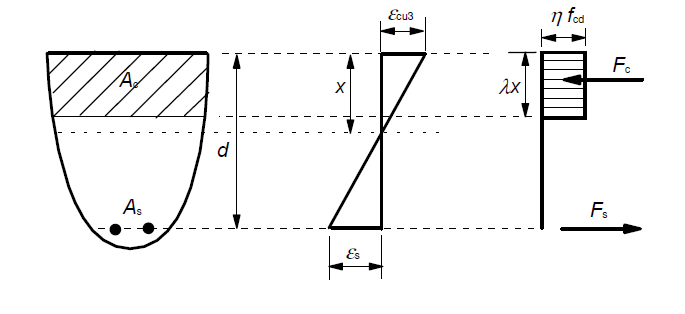
\includegraphics[width=0.9\textwidth]{Figuras/diagrama_tensoes_betao.png} 
    \caption{Diagrama retangular de tensões \cite{EN1992}.}
    \label{fig:diagrama_betao}
\end{figure}

\begin{figure}[htbp]
    \centering
    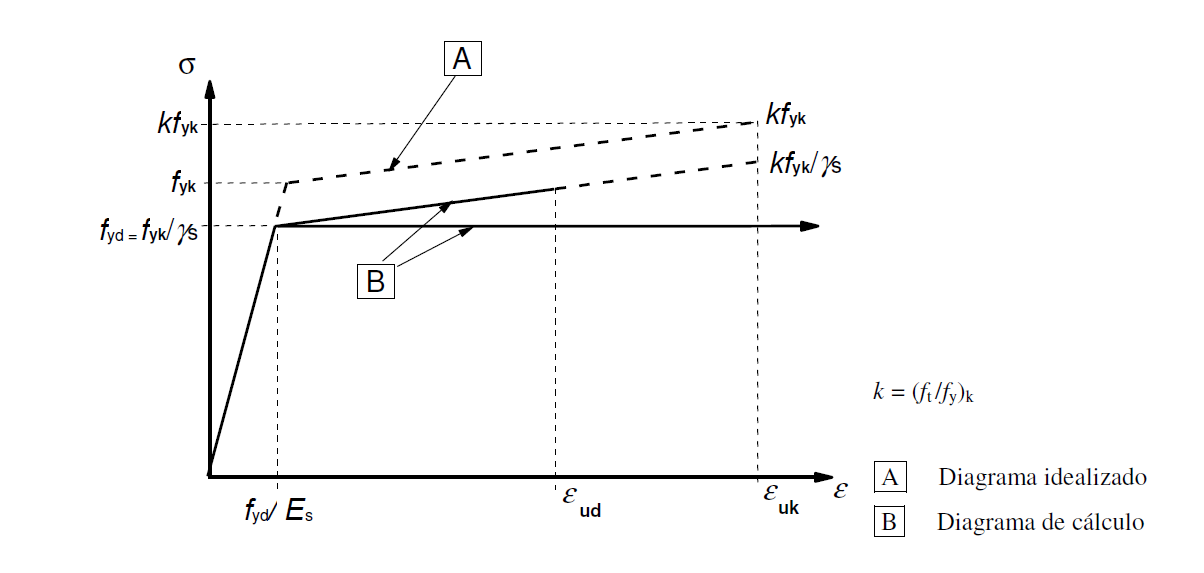
\includegraphics[width=0.9\textwidth]{Figuras/diagrama_aco.png} 
    \caption{Diagramas tensões-extensões, idealizado e de cálculo, do aço das armaduras para betão armado (tracionado ou comprimido) \cite{EN1992}.}
    \label{fig:diagrama_aco}
\end{figure}

\subsubsection{Procedimento de dimensionamento}
Enumeram-se a seguir os passos para efetuar o dimensionamento de elementos em betão armado, nomeadamente, os parâmetros dos materiais, a altura útil da secção, o momento fletor reduzido, a verificação de ductilidade, o cálculo da armadura, e as verificações finais.

\subsubsubsection{Definir as tensões limite para os materiais}
Calcular a tensão de cálculo do betão, através da seguinte expressão,
\begin{equation}
    f_{cd} = \alpha_{cc} f_{ck} / \gamma_{c}
\end{equation}
com  $\alpha_{cc}=1.0$ e $\gamma_{c}=1.5$.\\\\
Calcular a tensão de cedência do aço, com a expressão,
\begin{equation}
    f_{yd} = f_{yk} / \gamma_{s}
\end{equation}
com  $\gamma_{s}=1.15$.\\

\subsubsubsection{Altura útil da secção - $d$}
Assumindo uma estimativa inicial para os diâmetros da armadura, calcular,
\begin{equation}
    d = h - c_{nom} - \phi_{estribo} - \frac{\phi_{long}}{2}
\end{equation}

\subsubsubsection{Momento fletor reduzido - $\mu$}
O momento fletor reduzido caracteriza a solicitação da secção,
\begin{equation}
    \mu = \frac{M_{Ed}}{b \cdot d^{2} \cdot f_{cd}}
\end{equation}

\subsubsubsection{Verificação da ductilidade}
Para evitar armadura de compressão, verificar se $\mu \le \mu_{lim}$. Considerando o limite,
\begin{equation}
    \frac{x}{d} \le 0.45
\end{equation}
para garantir a ductilidade,
\begin{equation}
    \mu_{lim} = 0.8 \cdot 0.45 \cdot (1 - 0.5 \cdot 0.8 \cdot 0.45) \approx 0.295.
\end{equation}
Se $\mu > \mu_{lim}$, a secção deve ser redimensionada.

\subsubsubsection{Cálculo da área total das armaduras - $A_s$}
Calcular a profundidade reduzida do eixo neutro $\xi$ e o braço do binário $z$,
\begin{equation}
    \xi = \frac{1 - \sqrt{1 - 2\mu}}{\lambda},
\end{equation}
\begin{equation}
    z = d \cdot (1 - 0.5 \cdot \lambda \cdot \xi).
\end{equation}
A área de armadura necessária é,
\begin{equation}
    A_s = \frac{M_{Ed}}{z \cdot f_{yd}}
\end{equation}

\subsubsubsection{Verificações finais}
Garantir que,
\begin{equation}
    A_{s} \ge A_{s,min}
\end{equation}
e
\begin{equation}
    A_{s} \le 0.04 A_c
\end{equation}

\subsection{Pilar retangular sujeito a flexão composta reta}
Este modelo destina-se ao dimensionamento de pilares de secção retangular sujeitos a um esforço axial de compressão $N_{Ed}$, e a um momento fletor de cálculo $M_{Ed}$, segundo uma direção principal. O modelo integra a verificação de esbelteza e o cálculo dos efeitos de segunda ordem.

\subsubsection{Dados de Entrada}
\begin{enumerate}
    \item Geometria da secção:\\\\
    $b$ - Largura em \SI{}{mm};\\\\
    $h$ - Altura em \SI{}{mm};\\\\
    $l$ - Comprimento real em \SI{}{mm}.
    \item Condições de apoio:\\\\
    Para definir o coeficiente $\beta$ é necessário definir o tipo de ligação existente no topo e na base do pilar.
    \item Propriedades dos Materiais: \\\\
    $f_{ck}$ - Valor característico da tensão de rotura do betão à compressão aos 28 dias de idade em \SI{}{MPa};\\\\ 
    $f_{yk}$ - Valor característico da tensão de cedência à tração do aço das armaduras para betão armado em \SI{}{MPa};\\\\ 
    $c_{nom}$ - Recobrimento nominal em \SI{}{mm}.
    \item Esforços de cálculo:\\\\
    $N_{Ed}$ - Valor  de cálculo do esforço normal atuante (tração ou compressão) em \SI{}{kN};\\\\
    $M_{Ed}$ - Valor  de cálculo do momento fletor atuante em \SI{}{kNm};\\\\
    $M_{0Ed}$ - Valor do momento fletor de primeira ordem, incluindo o efeito de imperfeições em \SI{}{kNm};\\\\
    $M_{2}$ - Valor do momento nominal de segunda ordem em \SI{}{kNm}.\\
    \item Fluência:\\\\
    Coeficiente de fluência efetivo $\varphi_{ef}$.
\end{enumerate}
Nota: o valor do módulo de elasticidade e/ou de outras constantes são estáticas no algoritmo.

\subsubsection{Procedimento de Cálculo}
Antes do dimensionamento da secção do pilar em betão armado é verificada a sua estabilidade.

\subsubsubsection{Parâmetros de cálculo}
Determinar $f_{cd}$ e $f_{yd}$ e converter os esforços para unidades consistentes (N, mm).

\subsubsubsection{Análise da esbelteza}
\begin{enumerate}
    \item Comprimento de Encurvadura - $l_0$: \\\\
    Determinar por,
    \begin{equation}
        l_0 = \beta \cdot l
    \end{equation}
    onde $\beta$ depende das condições de apoio, e.g.:\\\\
    $\beta=0.7$ para uma apoio encastrado-encastrado;\\\\
    $\beta=2.0$ para uma consola.
    \item Esbelteza - $\lambda$:\\\\
    Calcular o raio de giração,
    \begin{equation}
        i = h / \sqrt{12}
    \end{equation}
    e a esbelteza,
    \begin{equation}
        \lambda = l_0 / i
    \end{equation}
    O valor de $l_0$, para elementos isolados, pode ser determinado utilizando o ábaco apresentado na Figura \ref{fig:esquema_pilar} ou figura 5.7 da EC2-1-1.
    \item Esbelteza limite - $\lambda_{lim}$ \cite{EN1992,CachimBases}:
    \begin{equation}
        \lambda_{lim} = \frac{20 \cdot A \cdot B \cdot C}{\sqrt{n}}
    \end{equation}
    onde,
    \\ $n = N_{Ed} / (A_c f_{cd})$
    \\ $A = 1/(1+0.2\varphi_{ef})$
    \\ $B=1.1$
    \\ $C=0.7$
\end{enumerate}

\begin{figure}[htbp]
    \centering
    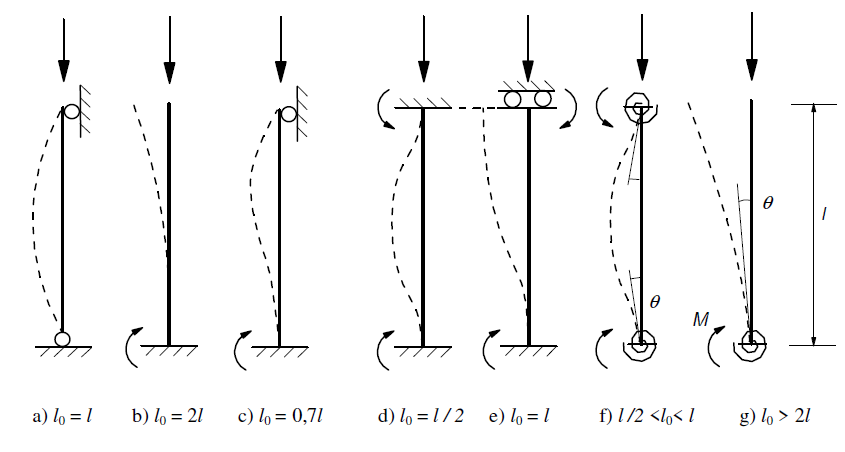
\includegraphics[width=1\textwidth]{Figuras/esquema_pilar_encurvadura.png}
    \caption{Esquema do comprimento de encurvadura para diferentes condições de apoio \cite{EN1992}.}
    \label{fig:esquema_pilar}
\end{figure}

\subsubsubsection{Cálculo do momento fletor - $M_{Ed}$}
Inicialmente $M_{Ed}$ é igual a $M_{0Ed}$.
Se $\lambda > \lambda_{lim}$, i.e., se se tratar de um pilar esbelto, calcular os efeitos de segunda ordem pelo método da curvatura nominal, i.e., calcular,
\begin{enumerate}
    \item a curvatura,
    \begin{equation}
        \frac{1}{r} = K_r \cdot K_{\varphi} \cdot \frac{1}{r_0}
    \end{equation}
    \item a excentricidade de segunda ordem,
    \begin{equation}
        e_2 = \frac{1}{r} \cdot l_0^2 \cdot \frac{1}{c}
    \end{equation}
    \item o momento adicional,
    \begin{equation}
        M_2 = N_{Ed} \cdot e_2
    \end{equation}
    \item e atualizar  o seu valor,
    \begin{equation}
        M_{Ed} = M_{0Ed} + M_2
    \end{equation}
\end{enumerate}

\subsubsubsection{Dimensionamento da armadura}
Com os esforços finais, $N_{Ed}$ e $M_{Ed}$, o método numérico procura, através de um processo iterativo de equilíbrio da secção, uma área de aço para betão $A_s$, tal que:
\begin{itemize}
    \item $N_{Rd} = N_{Ed}$ (equilíbrio axial)
    \item e $M_{Rd} \ge M_{Ed}$ (resistência em flexão composta).
\end{itemize}

\subsubsubsection{Seleção da armadura}
A solução final deve respeitar os limites de armadura mínima e máxima estabelecidos, dados por:
\begin{equation}
    A_{s,min} = \max\left(0.10 \frac{N_{Ed}}{f_{yd}};\, 0.002 A_c\right)
\end{equation}
\begin{equation}
    A_{s,max} = 0.04 A_c
\end{equation}
A área de armadura requerida é assim definida por:
\begin{equation}
    A_{s,req} = \max(A_s;\, A_{s,min})
\end{equation}
com $A_{s,req} \le A_{s,max}$. Por fim, a armadura deve ser disposta de forma simétrica na secção.

\subsection{Sapata isolada e centrada}
Este modelo aplica-se a sapatas de betão armado, de base retangular, suportando um pilar centrado. O procedimento divide-se em duas fases iterativas que a seguir se apresentam - dimensionamento geotécnico (SLS) e dimensionamento estrutural (ELU).

\subsubsection{Dimensionamento geotécnico - SLS}
O objetivo é determinar as dimensões em planta, $a$ e $b$, da sapata de maneira a satisfazer a tensão do solo.

\subsubsubsection{Cálculo dos esforços}
Converter os esforços dos ELU para os dos SLS, dividindo-os por um coeficiente médio, 
\begin{equation}
    \gamma_{G,avg} \approx 1.4
\end{equation}

\subsubsubsection{Ciclo iterativo para a  determinação das dimensões -  $a$ e $b$}
\begin{enumerate}
    \item Inicialmente estimar a área da sapata através do valor de $\sigma_{adm}$.
    \item Em cada iteração, adicionar o peso próprio da sapata às cargas, para determinar a carga total $N_{total}$.
    \item Calcular a excentricidade,
    \begin{equation}
        e = \frac{M_k}{N_{total}}
    \end{equation}
    \item Calcular as tensões no solo,
    \begin{equation}
        \sigma_{max,min} = \frac{N_{total}}{a \cdot b} \cdot \left(1 \pm \frac{6 \cdot e}{b}\right)
    \end{equation}
    \item O ciclo termina quando,
    \begin{equation}
        \sigma_{max} \le \sigma_{adm}
    \end{equation}
    e
    \begin{equation}
        \sigma_{min} \ge 0
    \end{equation}
    sem levantamento, e
    \begin{equation}
        e \le \frac{b}{6}
    \end{equation}
\end{enumerate}

\subsubsection{Dimensionamento estrutural - ELU}
Com a geometria definida na fase anterior, determinar a altura e a armadura da sapata.

\subsubsubsection{Tensão de cálculo}
Calcular
\begin{equation}
    \sigma_{Ed} = \frac{N_{Ed}}{a \cdot b}
\end{equation}
considerando uma distribuição uniforme.

\subsubsubsection{Altura da sapata - Punçoamento}
A altura da sapata é determinada iterativamente para resistir ao punçoamento sem armadura específica:
\begin{enumerate}
    \item Incrementar a altura útil $d$, ver \ref{fig:esquema_puncoamento}.
    \item Calcular o esforço atuante,
    \begin{equation}
        V_{Ed,pun} = N_{Ed} - \sigma_{Ed} \cdot A_{crit}
    \end{equation}
    \item Calcular a resistência $V_{Rd,c}$ do betão.
    \item A altura é válida quando,
    \begin{equation}
        V_{Rd,c} > V_{Ed,pun}
    \end{equation}
\end{enumerate}

\begin{figure}[htbp]
    \centering
    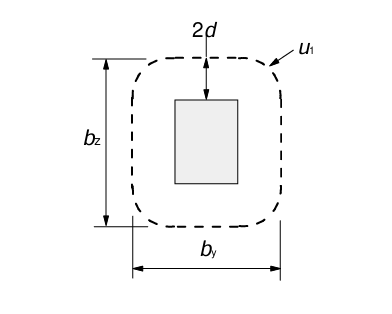
\includegraphics[width=0.6\textwidth]{Figuras/esquema_puncoamento.png}
    \caption{Perímetro de controlo crítico para a verificação ao punçoamento \cite{EN1992}}
    \label{fig:esquema_puncoamento}
\end{figure}

\subsubsubsection{Armaduras de flexão}
A sapata é calculada como consolas nas direções x e y. O momento nas faces do pilar é calculado, e de  seguida é dimensionada a armadura inferior, $A_{s,x}$ e $A_{s,y}$, usando o modelo de flexão simples.

\subsection{Métodos de otimização das armaduras}
Os modelos de otimização das armaduras são aplicados após o dimensionamento de vigas, pilares e sapatas. Os modelos permitem o cálculo da área de aço para betão $A_{s,req}$, através de algoritmos que respeitam as regras de pormenorização da EC2-1-1. Cada um dos modelos corresponde a um tipo de elemento.

\subsection{Otimização de armadura longitudinal (Modelo 1: Vigas e Pilares)}

O Modelo 1 aplica-se a vigas e pilares, baseando-se na otimização por \emph{barras discretas}. O objetivo é encontrar a combinação de varões comerciais (e.g., $4\phi16$) cuja área total $A_{s,\text{prov}}$ seja a mais próxima possível (por excesso) de $A_{s,\text{req}}$, respeitando os espaçamentos mínimos regulamentares.

\subsubsection{Dados de entrada}
\begin{itemize}
\item $A_{s,\text{req}}$: área teórica necessária [\si{cm^2}].
\item $l_d$: largura disponível para armadura:
\begin{equation}
l_d = b - 2(c_\text{nom} + \phi_\text{estribo}).
\end{equation}
\end{itemize}

\subsubsection{Verificação de espaçamento mínimo}
O espaçamento horizontal mínimo é:
\begin{equation}
s_h \geq \max(\phi_\text{long}; 20\,\si{mm}).
\label{eq:sh_min}
\end{equation}

\subsubsection{Geração e seleção de combinações}
O algoritmo gera combinações de varões comerciais por pares:
\begin{itemize}
\item \textbf{Vigas}: de 1 a 4 pares ($\phi$ único ou misto simétrico).
\item \textbf{Pilares}: mínimo 2 pares (garantindo simetria nas 4 faces).
\end{itemize}

De entre as combinações que satisfazem $A_{s,\text{prov}} \geq A_{s,\text{req}}$ e \eqref{eq:sh_min}, seleciona-se a de menor $A_{s,\text{prov}}$.

\subsection{Otimização de armadura distribuída (Modelo 2: Sapatas)}

Nas sapatas, a armadura é calculada por metro linear de largura (e.g., $\phi12@150$\si{mm}). O objetivo é minimizar a taxa de armadura $A_{s,\text{prov}}/m$.

\subsubsection{Dados de entrada}
\begin{itemize}
\item $A_{s,\text{req}}$: área necessária por metro [\si{cm^2/m}].
\item $l$: largura da faixa de cálculo (por defeito, $1\,\si{m}$).
\end{itemize}

\subsubsection{Algoritmo}
\begin{enumerate}
\item Iterar diâmetros comerciais ($\phi10$, $\phi12$, $\phi16$, ...).
\item Para cada $\phi$, calcular $n = \lceil A_{s,\text{req}}/A_\phi \rceil$.
\item Verificar se $n$ varões cabem em $1\,\si{m}$ respeitando espaçamentos.
\item Selecionar combinação com menor $A_{s,\text{prov}}$.
\item Converter em espaçamento: $s = \lfloor 1000/n \rfloor$\si{mm}.
\end{enumerate}


% Capítulo 4
\newpage
\section{ALGORITMOS DE DIMENSIONAMENTO IMPLEMENTADOS}
%Nas secções seguintes apresentam-se os algoritmos que implementam os modelos teóricos enunciados no capítulo anterior \cite{EN1992,CachimPreEforco}. Os algoritmos escritos em pseudocódigo pretendem representar uma maneira simples de como fazer a implementação dos modelos teóricos para uma linguagem de programação qualquer. Porém, no trabalho desenvolvido estes são escritos em  Python, integrados na framework web Django, para possibilitar o alojamento da aplicação num servidor e tornando-a, assim, acessível a toda a comunidade científica e académica.

Este capítulo apresenta os algoritmos computacionais derivados dos modelos teóricos do Capítulo 3. 
Cada algoritmo é expresso em pseudocódigo, destacando as iterações de refinamento, verificações normativas e otimização construtiva \cite{EN1992,CachimPreEforco}.

\subsection{Algoritmo para o dimensionamento de vigas em flexão simples}
%O algoritmo listado em Listing \ref{alg:viga}, descreve o procedimento implementado num módulo Django de nome \texttt{viga\_service.py}. Diferente de um cálculo manual simplificado, o programa executa uma iteração de refinamento. Inicialmente, iteração 1, assume-se um diâmetro para uma armadura para estimar a altura útil $d_1$. Após calcular a armadura necessária, o sistema verifica qual o diâmetro comercial ótimo para essa área. Se este diâmetro real diferir do assumido, o sistema recalcula tudo, iteração 2, com a altura útil corrigida $d_2$, eliminando erros de estimativa.
O algoritmo \texttt{viga\_service.py} implementa a iteração de refinamento da altura útil $d$, eliminando erros de estimativa.

\begin{lstlisting}[style=PseudoStyle, basicstyle=\ttfamily\normalsize, caption={Dimensionamento de uma viga à flexão simples (viga\_service.py)}, label={alg:viga}]
ALGORITMO Dimensionar_Viga
ENTRADAS: b, h, f_ck, f_yk, M_Ed, c_nom
CONSTANTES: gamma_c=1.5, gamma_s=1.15, alpha_cc=1.0, lambda=0.8

// 1. Parametros de Calculo
f_cd <- alpha_cc * f_ck / gamma_c
f_yd <- f_yk / gamma_s
phi_estribo <- 8.0
phi_long_assumido <- 16.0 // Estimativa inicial

// --- ITERACAO 1 (Estimativa) ---
// 3. Altura util estimada
d1 <- h - c_nom - phi_estribo - (phi_long_assumido / 2)

// 4. Momento reduzido e Verificacao de Ductilidade
mu <- M_Ed / (b * d1^2 * f_cd)
mu_lim <- 0.8 * 0.45 * (1 - 0.5 * 0.8 * 0.45)
SE mu > mu_lim ENTAO
    ERRO "Seccao necessita de armadura de compressao"
FIM SE

// 7. Area de Aco Temporaria
xi <- (1 - SQRT(1 - 2 * mu)) / 0.8
z <- d1 * (1 - 0.5 * 0.8 * xi)
As_req_temp <- M_Ed / (z * f_yd)

// Determinar diametro real da solucao otima temporaria
solucao_temp <- Otimizar_Armadura(As_req_temp, largura_disp)
phi_long_final <- Obter_Diametro(solucao_temp)

// --- ITERACAO 2 (Recalculo de Precisao) ---
SE phi_long_final != phi_long_assumido ENTAO
    // 6.1 Nova Altura util (Refinada)
    d2 <- h - c_nom - phi_estribo - (phi_long_final / 2)
    
    // 6.2 Recalculo de Esforcos
    mu <- M_Ed / (b * d2^2 * f_cd)
    SE mu > mu_lim ENTAO ERRO "Excede mu_lim no recalculo"
    
    xi <- (1 - SQRT(1 - 2 * mu)) / 0.8
    z <- d2 * (1 - 0.5 * 0.8 * xi)
    As_req <- M_Ed / (z * f_yd)
SENAO
    As_req <- As_req_temp
FIM SE

// 8. Verificacao de Armadura Minima
f_ctm ← 0.30 * f_ck^(2/3)
A_s,min ← max(0.26 * (f_ctm/f_yk) * b * d₂, 0.0013 * b * d₂)
A_s,final ← max(A_s,req, A_s,min)

// 9. Proposta Final (Servico de Armadura)
combinações ← Otimizar_Armadura(A_s,final, largura_disp)
RETORNAR combinações (única e mista)
\end{lstlisting}


\subsection{Algoritmo para dimensionamento de pilares em flexão composta}
%O algoritmo listado em Listing \ref{alg:pilar} descreve o procedimento implementado num módulo Django de nome \texttt{pilar\_service.py}. 
%A maior dificuldade encontrada na sua implementação foi a verificação automática da instabilidade. O algoritmo calcula a esbelteza $\lambda$, e compara-a com o limite $\lambda_{lim}$. Se o pilar for esbelto, o algoritmo calcula a curvatura $1/r$, e o momento de segunda ordem $M_2$, antes de avançar para o cálculo da área da armadura.
O algoritmo \texttt{pilar\_service.py} integra verificação de esbelteza e efeitos de 2ª ordem (método da curvatura nominal) ver listagem 2.

\begin{lstlisting}[style=PseudoStyle, basicstyle=\ttfamily\normalsize, caption={Dimensionamento de pilares à flexão composta reta (pilar\_service.py)}, label={alg:pilar}]
ALGORITMO Dimensionar_Pilar
ENTRADAS: b, h, l₀, ligações, f_ck, f_yk, N_Ed, M₀_Ed, c_nom, φ_ef

// 1. Comprimento de encurvatura
β ← Determinar_Beta(lig_top, lig_base)  // 0.7, 0.85, 1.0
l₀ ← β * l

// 2. Esbelteza
i ← h / √12
λ ← l₀ / i
n ← N_Ed / (b * h * f_cd)
λ_lim ← 20 * A * B * C / √n

// 3. Efeitos de 2ª ordem 
M_Ed ← M₀_Ed
SE λ > λ_lim ENTAO
  1/r ← K_r * K_φ * (f_yd/E_s) / (0.45 * d_est)
  e₂ ← (1/r) * l₀² / 10
  M₂ ← N_Ed * e₂
  M_Ed ← M₀_Ed + M₂
FIM SE

// 4. Dimensionamento iterativo
A_s,req ← Dimensionar_Pilar_Rigoroso(N_Ed, M_Ed, ...)

// 5. Mínimos e otimização
A_s,min ← max(0.10 * N_Ed / f_yd, 0.002 * b * h)
A_s,final ← max(A_s,req, A_s,min)
combinações ← Otimizar_Armadura_Pilar(A_s,final)
RETORNAR combinações simétricas
\end{lstlisting}

%A implementação em Python do dimensionamento de pilares segue diretamente o procedimento apresentado na Secção dos pilares em flexão composta. A função \texttt{dimensionar\_pilar(...)} começa por calcular os parâmetros de cálculo $f_{cd}$, $f_{yd}$, a área de betão $A_c = b \cdot h$ e os esforços de dimensionamento $N_{Ed}$ e $M_{0Ed}$. Em seguida avalia a esbelteza do elemento, através do comprimento de encurvadura $l_0 = \beta l$, do raio de giração $i = h / \sqrt{12}$, da esbelteza $\lambda = l_0 / i$ e do esforço axial reduzido $n = N_{Ed} / (A_c f_{cd})$, determinando também a esbelteza limite $\lambda_{lim}$ pela expressão simplificada adotada. A comparação entre $\lambda$ e $\lambda_{lim}$ permite classificar o pilar como não esbelto ou esbelto. No primeiro caso, o momento de cálculo mantém-se igual ao momento de primeira ordem ($M_{Ed} = M_{0Ed}$); no segundo, é ativado o método da curvatura nominal, sendo calculado um incremento de segunda ordem $M_2$ e definido o momento total $M_{Ed} = M_{0Ed} + M_2$. Este valor é então utilizado na função auxiliar \texttt{\_dimensionar\_pilar\_rigoroso(...)}, que implementa o modelo teórico: itera na profundidade da zona comprimida $x$ até satisfazer o equilíbrio axial $N_{Rd} = N_{Ed}$, calcula o momento resistente correspondente $M_{Rd}$ e ajusta a área total de armadura $A_s$ até garantir a condição $M_{Rd} \ge M_{Ed}$. Por fim, a área de armadura obtida é confrontada com os limites mínimos e máximos (entre $A_{s,min}$ e $A_{s,max} = 0.04 A_c$), sendo definido o valor final $A_{s,req}$, que é então passado ao módulo de otimização de armaduras para seleção da combinação de varões mais económica.

\newpage
\subsection{Algoritmo para dimensionamento de sapatas}

%O algoritmo listado em Listing \ref{alg:sapata} descreve o procedimento implementado num módulo Django de nome \texttt{sapata\_service.py}. O módulo distingue-se pelo uso de dois ciclos iterativos:
%\begin{enumerate}
    %\item Ciclo geotécnico - SLS:\\
    %Itera as dimensões em planta $a$ e $b$, até garantir que a tensão no solo $\sigma_{max}$, é inferior à admissível e que a sapata não levanta $\sigma_{min} \ge 0$.
    %\item Ciclo Estrutural - ELU:\\
    %Itera a altura útil $d$, incrementando-a passo a passo, de um em um cm, até verificar a segurança ao punçoamento sem armadura específica.
%\end{enumerate}

O algoritmo \texttt{sapata\_service.py} implementa \emph{dupla iteração}: geotécnica (ELS) para a determinação das dimensões em planta $A$ e $B$, seguida de estrutural (ELU) para a determinação da altura $H$ via punçoamento ver listagem 3. 

\begin{lstlisting}[style=PseudoStyle, basicstyle=\ttfamily\normalsize, caption={Dimensionamento de sapatas (sapata\_service.py)}, label={alg:sapata}]
ALGORITMO Dimensionar_Sapata
ENTRADAS: sigma_adm, f_ck, f_yk, N_Ed, M_Ed, dimensoes_pilar

// --- FASE 1: DIMENSIONAMENTO GEOTECNICO (ELS) ---
N_k <- N_Ed / 1.4
M_k <- M_Ed / 1.4
Area_req <- N_k / sigma_adm
// Estimativa inicial de A e B baseada na area e proporcao do pilar
A, B <- Estimar_Geometria(Area_req, proporcao_pilar)
PARA i DE 1 ATE 50 FAZER:
    H_est <- MAX(A, B) / 8
    Peso_Proprio <- A * B * H_est * 25
    N_total <- N_k + Peso_Proprio
    e_y <- M_k / N_total
    
    sigma_max <- (N_total / A*B) * (1 + 6*e_y/B)
    sigma_min <- (N_total / A*B) * (1 - 6*e_y/B)
    
    // Criterios de paragem: Tensao OK e sem levantamento excessivo
    SE (sigma_max <= sigma_adm) E (sigma_min >= 0) E (e_y <= B/6) ENTAO
        SAIR DO CICLO
    SENAO
        Incrementar B em 0.05m
        Ajustar A proporcionalmente
    FIM SE
FIM PARA

// --- FASE 2: DIMENSIONAMENTO ESTRUTURAL (ELU) ---
// Tensao de calculo no solo (desprezando peso proprio a favor da seguranca)
sigma_Ed <- N_Ed / (A * B)
// Iteracao para Altura Util (Puncoamento)
d <- 0.15 // Inicio com 15cm
PARA i DE 1 ATE 50 FAZER:
    // Perimetro critico u1 e Area critica
    u1 <- 2*(c1+c2) + 2*PI*d
    Acrit <- ... // Area dentro do perimetro de controlo
    V_Ed_pun <- N_Ed - sigma_Ed * Acrit
    
    // Resistencia ao corte (sem armadura)
    k <- MIN(1 + SQRT(200/d), 2.0)
    V_Rd_c <- (0.18/gamma_c) * k * (100 * 0.005 * f_ck)^(1/3) * u1 * d
    
    SE V_Rd_c >= V_Ed_pun ENTAO
        SAIR DO CICLO
    SENAO
        d <- d + 0.01 // Incrementa 1cm
    FIM SE
FIM PARA
H_final <- Arredondar_Superior(d + c_nom + phi/2)

// --- FASE 3: FLEXAO (Modelo de Consolas) ---
lx <- (A - bp) / 2
M_Ed_flex <- (sigma_Ed * lx^2) / 2
As_req <- Dimensionar_Flexao(M_Ed_flex, d)

RETORNAR Geometria(A, B, H) e Armaduras(Ax, Ay)
\end{lstlisting}

\subsection{Algoritmo para a otimização de armadura}
O algoritmo listado em Listagem \ref{alg:otimizacao} descreve a metodologia de decisão utilizada para converter uma área de aço para betão teórica $A_{s,req}$, numa solução construtiva prática. Este algoritmo varia consoante o elemento:
\begin{enumerate}
    \item Vigas e pilares\\
    Gera combinações de varões, verifica se cabem na largura disponível e escolhe a que tem menor área total. Para pilares, impõe ainda simetria e número par de varões.
    \item Sapatas\\
    Itera sobre os diâmetros para encontrar o espaçamento necessário e escolhe a solução com menor consumo de aço por metro linear.
\end{enumerate}

\begin{lstlisting}[style=PseudoStyle, basicstyle=\ttfamily\normalsize, caption={Otimização de Armadura (armadura\_service.py)}, label={alg:otimizacao}]
ALGORITMO Otimizar_Armadura
ENTRADAS: As_req, largura_disponivel, tipo_elemento

// --- CASO 1: VIGAS E PILARES (Combinacoes de Varoes) ---
SE tipo_elemento == "Viga" OU "Pilar" ENTAO
    solucoes_validas <- []
    diametros <- [10, 12, 16, 20, 25]
    
    // Gerar combinacoes de 2 a 8 varoes
    // (Para Pilares: apenas numeros pares 4, 6, 8)
    PARA num_barras DE min_barras ATE 8 FAZER:
        
        // Testar combinacoes de diametro Unico e Misto
        combinacoes <- Gerar_Combinacoes(diametros, num_barras)
        
        PARA comb EM combinacoes FAZER:
            As_total <- Soma_Areas(comb)
            
            // Verifica se cumpre a area necessaria
            SE As_total >= As_req ENTAO
                // Verifica se cumpre espacamentos minimos
                espaco_nec <- Calcular_Largura_Nec(comb)
                SE espaco_nec <= largura_disponivel ENTAO
                    Adicionar comb a solucoes_validas
                FIM SE
            FIM SE
        FIM PARA
    FIM PARA
    // Criterio de decisao: Menor Area Total (Economia)
    RETORNAR Menor_Area(solucoes_validas)

// --- CASO 2: SAPATAS (Barras por Metro) ---
SENAO SE tipo_elemento == "Sapata" ENTAO
    solucoes_validas <- []
    PARA diam EM [10, 12, 16, 20, 25] FAZER:
        area_unitaria <- Area(diam)
        // Calcular numero de barras por metro
        n_barras <- CEIL(As_req / area_unitaria)
        As_prov <- n_barras * area_unitaria
        
        // Verificar espacamento resultante
        espacamento <- 1000 / n_barras
        SE espacamento >= esp_minIMO ENTAO
            Adicionar (diam, As_prov) a solucoes_validas
        FIM SE
    FIM PARA
    RETORNAR Menor_Area(solucoes_validas)
FIM SE
\end{lstlisting}

% Capítulo 5
\newpage
\section{DESCRIÇÃO DA IMPLEMENTAÇÃO DOS ALGORITMOS EM PYTHON}

Este capítulo descreve o processo de implementação dos algoritmos de dimensionamento, detalhados nos capítulos anteriores. 
Descreve-se a seguir a arquitetura aplicação desenvolvida, as tecnologias utilizadas e a tradução da lógica de cálculo em código python.

\subsection{Arquitetura e tecnologia}
O desenvolvimento e implementação da aplicação baseia-se numa arquitetura modular, dividida entre o \textit{Backend}, onde se integra a lógica de cálculo e de dados, 
e o \textit{Frontend}, onde se integra a interface de interação entre utilizador e aplicação, ver a estrutura de ficheiros apresentada em Listing 5.

\subsubsection{Arquitetura MVT e Serviços}
A aplicação foi construída sobre a framework web Django \cite{DjangoDocs}, baseada na linguagem Python. 
O Django adota o padrão de desenho de software Modelo-Vista-Template (MVT), que promove o desenvolvimento rápido e um \textit{design} pragmático através da separação de responsabilidades. 
No contexto desta aplicação, o padrão MVT organiza-se da seguinte forma:

%\begin{enumerate}
    \begin{enumerate}
        \item \textbf{Modelo (Model):} É a camada de acesso aos dados. Define a estrutura da base de dados através de classes Python simples, abstraindo a complexidade de transacionar SQL diretamente. Na aplicação desenvolvida, os modelos gerem, por exemplo, o registo do histórico de cálculos do utilizador (\texttt{HistoricoCalculo}) e as configurações visuais do sistema (\texttt{SystemConfiguration}).
        \item \textbf{Vista (View):} É o "cérebro" da resposta web. Recebe o pedido HTTP feito pelo utilizador (por exemplo, a submissão do formulário de dimensionamento de uma viga), orquestra o processamento desses dados (comunicando com os Modelos ou com a camada de Serviços) e, no final, seleciona qual o Template a ser renderizado com os resultados da operação para devolver como resposta.
        \item \textbf{Template:} Corresponde à camada de apresentação ao utilizador (frontend). Consiste em ficheiros HTML dinâmicos que utilizam uma linguagem de \textit{tags} própria (Django Template Language) para colocar as variáveis calculadas geradas pela Vista no sítio certo do interface gráfico.
    \end{enumerate}
%\end{enumerate}

Para fazer face à especificidade de engenharia do presente trabalho, a arquitetura MVT padrão do Django foi complementada por uma camada de \textbf{Serviços} explícita. Esta decisão arquitetural visa encapsular a pesada complexidade matemática dos algoritmos de dimensionamento estrutural, isolando-a da lógica de encaminhamento web das \textit{Views}. Esta abordagem modular garante um código mais testável, escalável e com uma clara separação de responsabilidades, e encontra-se ilustrada na Figura \ref{fig:arquitetura_mvt_cap5}.

\begin{figure}[H]
  \centering
  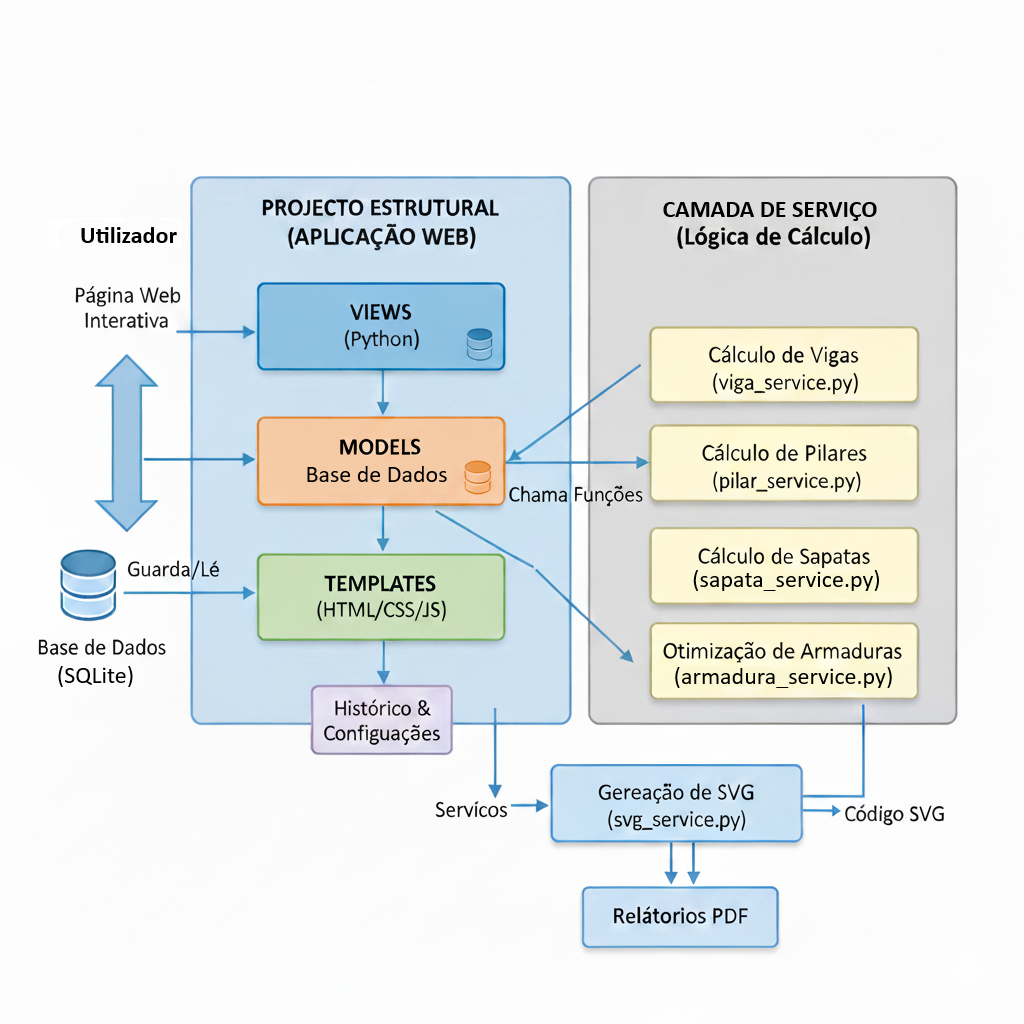
\includegraphics[width=1\textwidth]{Figuras/arquitetura_mvt.png}
  \caption{Diagrama da arquitetura MVT + Serviços da aplicação desenvolvida.}
  \label{fig:arquitetura_mvt_cap5}
\end{figure}

\subsubsection{Tecnologias Backend}
\begin{enumerate}
    \item \textbf{Python 3.10} \cite{PythonDocs}: linguagem base, adequada a cálculos numéricos.
    \item \textbf{Django ORM}: abstrai operações SQL para modelos como \texttt{HistoricoCalculo}.
    \item \textbf{Serviços modulares}: lógica EC2 isolada em \texttt{services/}, facilitando testes unitários.
\end{enumerate}

\subsubsection{Tecnologias Frontend}
\begin{enumerate}
\item \textbf{Templates Django}: HTML dinâmico com injeção de dados dos serviços.
\item \textbf{CSS3}: variáveis personalizáveis para temas claro/escuro.
\item \textbf{SVG}: geração vetorial de desenhos técnicos \cite{DaileySVG}.
\item \textbf{JavaScript}: validação de formulários e interatividade \cite{PortelaAvancado,MDNWeb}.
\end{enumerate}

\newpage
\begin{lstlisting}[basicstyle=\ttfamily\normalsize, moredelim={[is][\color{blue}\bfseries]{@}{@}}, morecomment={[l]\#}, commentstyle=\color{codegreen}\itshape, caption={Estrutura de ficheiros do projeto Django}, label={lst:estrutura_1}]

@TeseFinal/@
|-- manage.py
|-- requirements.txt
|-- @projeto_estrutural/@
|   |-- settings.py
|   |-- urls.py
|   |-- wsgi.py
|   |-- asgi.py
|-- @calculos/@
    |-- models.py                   # Base de Dados
    |-- views.py                    # Controlador HTTP
    |-- urls.py
    |-- forms.py
    |-- tests.py
    |-- @services/@                   # Camada de Servicos
        |-- viga_service.py
        |-- pilar_service.py
        |-- sapata_service.py
        |-- armadura_service.py
    |-- @templates/calculos/@          # Interface
    |   |-- base.html
    |   |-- index.html
    |   |-- viga_dimensionamento.html
    |   |-- pilar_dimensionamento.html
    |   |-- sapata_dimensionamento.html
    |   |-- historico.html
    |   |-- historico_detalhe.html
    |   |-- configuracao.html
    |   |-- relatorio_pdf.html
    |-- @static/calculos/@            # Temas visuais
        |-- style.css
        |-- @icons/@
            |-- artic.svg
            |-- encab.svg
            |-- livre.svg
\end{lstlisting}

\subsection{Implementação dos algoritmos}

A tradução dos modelos teóricos, apresentados no capítulo 4, para código Python são seguidamente apresentados:

\begin{enumerate}
    \item Algoritmo 1 - viga:\\
    O \texttt{viga\_service.py} implementa o dimensionamento completo à flexão simples. O algoritmo inicia-se com a verificação dos limites de ductilidade, momento reduzido $\mu$. A sua principal característica é o ciclo de \textit{refinamento automático}. Após uma estimativa inicial, o sistema identifica o diâmetro da solução ótima e, se este diferir do assumido, recalcula a altura útil $d$, e a área de aço para betão necessária, garantindo total coerência entre o cálculo e a solução construtiva. Por fim, valida a área obtida comparando-a com a armadura mínima regulamentar.

    \item Algoritmo 2 - pilar:\\
    O \texttt{pilar\_service.py} contém a lógica para a análise de estabilidade. Verifica a esbelteza $\lambda$, e, se necessário, aplica o Método da Curvatura Nominal para calcular os efeitos de segunda ordem. A função \texttt{\_dimensionar\_pilar\_rigoroso} utiliza um método numérico iterativo para encontrar a profundidade do eixo neutro e o momento resistente da secção.

    \item Algoritmo 3 - sapata:\\
    O \texttt{sapata\_service.py} reflete a dupla iteração sequencial.
    Primeiro, um ciclo geotécnico (SLS) ajusta as dimensões em planta $A$ e $B$ até satisfazer as tensões no solo. Segundo, um ciclo estrutural (ELU) incrementa a altura $d$, até verificar a segurança ao punçoamento sem armadura específica.

    \item Algoritmo 4 - otimização:\\
    A lógica de seleção da armadura está implementada em \texttt{armadura\_service.py}, para vigas e pilares, e integrada no serviço das sapatas. O algoritmo gera todas as combinações possíveis de varões comerciais, filtra-as pelo cumprimento das áreas e dos espaçamentos regulamentares, e seleciona automaticamente a solução com menor consumo de aço.
\end{enumerate}

\subsection{Funcionalidades gráficas entre outras}
Para além do cálculo numérico, implementaram-se lógicas específicas para a geração de outputs profissionais.

\subsubsection{Lógica de geração da representação gráfica SVG}
O sistema utiliza o formato SVG (\textit{Scalable Vector Graphics}) para criar os desenhos técnicos \cite{DjangoDocs,DaileySVG,TikZManual,TikZGoncalves}. Ao contrário de uma imagem comum, como uma fotografia, o SVG não é um conjunto de pixeis, mas sim um conjunto de {instruções geométricas, como linhas, círculos e retângulos, definidas matematicamente. O processo de geração é automático e segue uma lógica sequencial que liga os resultados do cálculo ao desenho final.

\subsubsubsection{Ponte entre o cálculo e o desenho - Preparação dos dados}
Imediatamente após a execução do algoritmo de dimensionamento e de encontrar a solução ótima, ver capítulo 4, o sistema empacota os resultados num dicionário de dados específico, chamado \texttt{dados\_desenho}. Este dicionário atua como um guião ou folha de obra para o desenhador automático, contendo apenas as informações essenciais:

\begin{enumerate}
    \item Geometria:\\
    As dimensões finais validadas, e.g., $b = \SI{300}{mm}$, $h = \SI{500}{mm}$, para vigas, ou $a = \SI{2.3}{m}$, $b = \SI{2.3}{m}$, para sapatas.
    \item Armaduras:\\
    A solução construtiva escolhida, e.g., $n = 4$, $\phi_{lg} = 16$ para pilares ou $\phi = 12$ e $s = \SI{15}{cm}$ para a sapatas.
    \item Detalhes:\\
    O recobrimento nominal $c_{nom}$, e diâmetros dos estribos, $\phi$.
\end{enumerate}

O dicionário de dados é enviado para as funções de desenho, garantindo uma representação da secção transversal conforme.

\subsubsubsection{Definição da tela digital - ViewBox}
Antes de traçar qualquer linha, o código lê as dimensões geométricas, e.g., $b$ e $h$ do pacote de dados e define uma tela digital / virtual. O tamanho desta tela adapta-se dinamicamente às dimensões do elemento contando com uma margem de segurança \textit{padding}, garantindo que o desenho nunca fica cortado, independentemente da secção transversal da viga ter $\SI{20}{cm}$ ou $\SI{1}{m}$ de altura.

\subsubsubsection{Desenho da viga em flexão simples}
A função \texttt{desenhar\_viga\_svg} lê os dados e desenha por camadas:
\begin{enumerate}
    \item O betão:\\
    Desenha um retângulo de cor cinza com as dimensões exatas $b \times h$ lidas dos dados de entrada.
    \item Os estribos:\\
    Calcula as coordenadas internas subtraindo o recobrimento $c_{nom}$ às bordas. Desenha um retângulo transparente com cantos arredondados para simular a dobragem do aço.
    \item A Armadura principal:\\
    É lido o número de varões $n$, e o diâmetro $\phi$. Calcula-se o espaço livre dentro do estribo, divide-o por $n-1$ e desenha $n$ círculos de cor preto, com diâmetro proporcional a $\phi$, perfeitamente equidistantes na base da secção.
\end{enumerate}

\subsubsubsection{Desenho do pilar em flexão composta reta - Simetria}
O pilar segue a mesma lógica definida anteriormente para vigas. Porém, a colocação dos varões é gerida por um algoritmo de simetria:
\begin{enumerate}
    \item Cantos:\\
    O código coloca automaticamente um varão em cada um dos quatro cantos do estribo.
    \item Faces laterais:\\
    Se o cálculo exigir mais do que 4 varões, e.g., 8 varões, o código calcula o espaço disponível entre os cantos e distribui os varões restantes equitativamente pelas quatro faces, assegurando a simetria exigida pelo modelo de cálculo.
\end{enumerate}

\subsubsubsection{Desenho da sapata - Vistas ortogonais}
Para a sapata, geram-se dois desenhos distintos para facilitar a leitura:
\begin{enumerate}
    \item Vista em planta:\\
    Desenha a sapata, retângulo $a \times b$, e o pilar ao centro. De seguida, lê o espaçamento calculado $s$, e desenha linhas cruzadas, i.e., uma grelha, representando a malha de aço, parando o desenho exatamente nas margens definidas pelo recobrimento.
    \item Vista em corte:\\
    Desenha o perfil lateral com a altura $h$. Na base, desenha uma fila de círculos que representam os varões cortados, permitindo ao utilizador visualizar a altura útil $d$, e confirmar que a armadura está corretamente posicionada na zona tracionada.
\end{enumerate}

\subsubsection{Lógica de geração de relatórios em  formato PDF}
A capacidade de exportar uma solução completa é fundamental em engenharia. A app não desenha o PDF do zero. Em vez disso, utiliza uma abordagem de conversão inteligente:
\begin{enumerate}
    \item O template de impressão:\\
    Foi criado um ficheiro HTML específico, \texttt{relatorio\_pdf.html}, que atua como uma folha de papel digital. O template não tem botões nem menus de navegação, apenas o cabeçalho, os dados técnicos formatados e as imagens SVG.
    \item O motor de conversão:\\
    Quando o utilizador clica em Exportar PDF, a vista utiliza a biblioteca \textit{WeasyPrint}. Esta ferramenta atua como um navegador invisível, ela lê, o HTML e o CSS do relatório, e imprime-o digitalmente para um ficheiro PDF, preservando a vetorização dos desenhos técnicos.
\end{enumerate}

\subsubsection{Histórico de cálculos - Persistência de dados}
Para garantir que nenhum dimensionamento se perde, a app implementa um mecanismo de persistência:
\begin{enumerate}
    \item O diário de bordo - Base de dados:\\
    O modelo \texttt{HistoricoCalculo} funciona como um arquivo digital. Sempre que um cálculo é concluído com sucesso, o sistema guarda instantaneamente dois pacotes de informação em formato JSON: o \texttt{input\_data}, o que o utilizador inseriu, e o \texttt{resultado\_final}, o que o sistema calculou.
    \item A recuperação:\\
    Quando o utilizador acede ao menu "Histórico", o sistema consulta o arquivo \texttt{HistoricoCalculo} e reconstrói a lista de todos os cálculos passados, permitindo reabrir qualquer um deles e ver os detalhes exatos como se tivessem acabado de ser gerados.
\end{enumerate}

\subsubsection{Personalização da interface - \textit{Context processor}}
A funcionalidade que permite ao utilizador mudar o tema, claro / escuro, ou a cor principal da aplicação baseia-se num mecanismo global do Django:
\begin{enumerate}
    \item Configuração centralizada:\\
    As preferências do utilizador são guardadas numa tabela única \texttt{SystemConfiguration}.
    \item Injeção global de estilos:\\
    Foi criado uma \textit{Context processor}, que é uma função especial que corre antes de cada página carregar. Esta função verifica as configurações guardadas e injeta as variáveis de cor e imagem de fundo diretamente no cabeçalho de todas as páginas HTML. Desta forma, quando o utilizador altera a cor de azul para vermelho, o sistema não precisa de alterar centenas de ficheiros, apenas muda uma variável na base de dados e toda a app reage instantaneamente.
\end{enumerate}

\subsection{Apresentação da interface e fluxo de utilização}
\label{sec:interface}

A aplicação foi desenhada para guiar o utilizador através de um fluxo de trabalho lógico. Apresenta-se de seguida o funcionamento de cada módulo, focando-se na introdução de dados. As interfaces completas, com os resultados gerados, podem ser consultadas no Anexo A.

\subsubsection{Menu Principal}

O ponto de entrada é o Menu Principal (Figura \ref{fig:menu_principal}), que centraliza o acesso a todas as funcionalidades do sistema.

\begin{figure}[htbp]
    \centering
    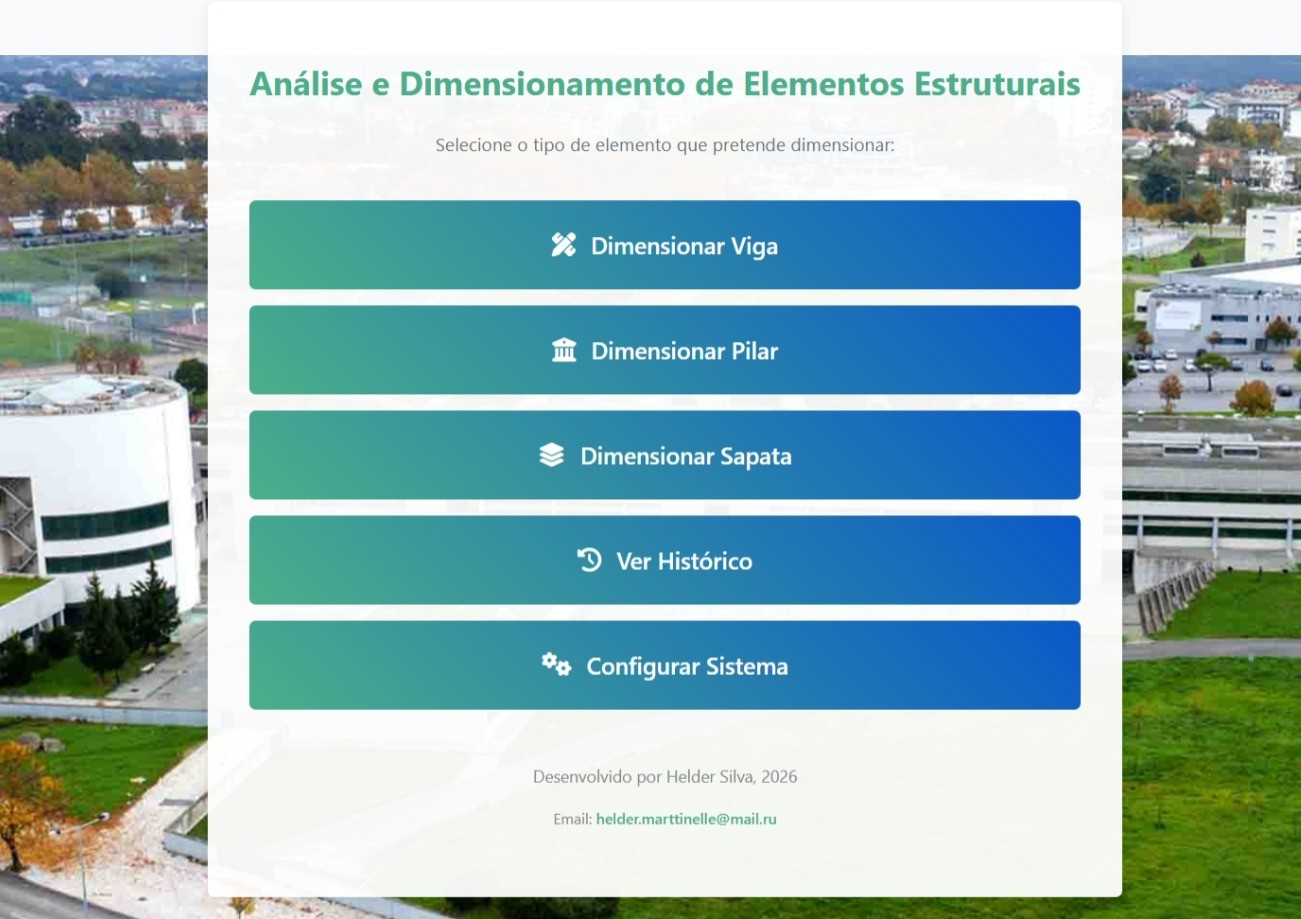
\includegraphics[width=0.9\textwidth]{Figuras/Menu_Inicial.jpg}
    \caption{Menu principal da aplicação com acesso aos módulos de dimensionamento.}
    \label{fig:menu_principal}
\end{figure}

\newpage
\subsubsection{Módulo de Vigas}
\paragraph{Entrada de Dados}

O formulário solicita as características geométricas da secção ($b, h$), as propriedades dos materiais (classes de betão e aço) e o esforço de cálculo ($M_{Ed}$) ver Figura \ref{fig:viga_input}.

\begin{figure}[htbp]
    \centering
    {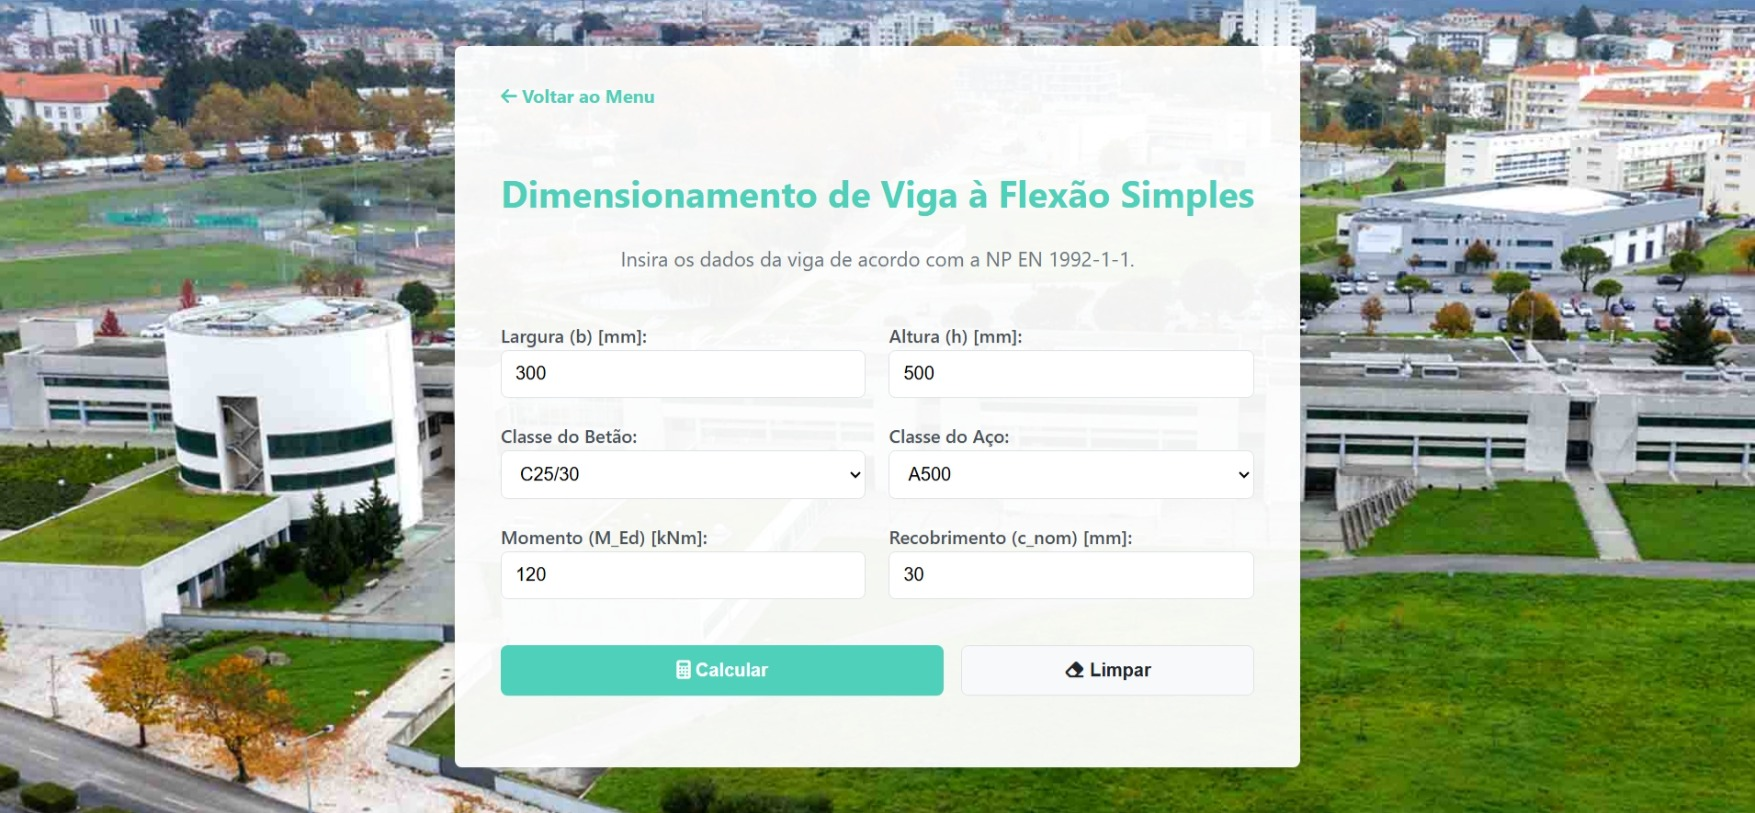
\includegraphics[width=0.89\textwidth]{Figuras/Viga.jpg}}
    \caption{Formulário de entrada de dados para o dimensionamento de elementos do tipo viga.}
    \label{fig:viga_input}
\end{figure}

\paragraph{Visualização de Resultados}
Após o cálculo iterativo, a aplicação apresenta a solução ótima de armadura e o desenho vetorial da secção. A visualização completa da interface com os resultados encontra-se no apêndice I.

\subsubsection{Módulo de Pilares}

\paragraph{Entrada de Dados}
Além da geometria e materiais, o utilizador define as condições de fronteira no topo e na base através de ícones gráficos, essenciais para o cálculo da esbeltez, ver Figura \ref{fig:pilar_input}.

\begin{figure}[htbp]
    \centering
    {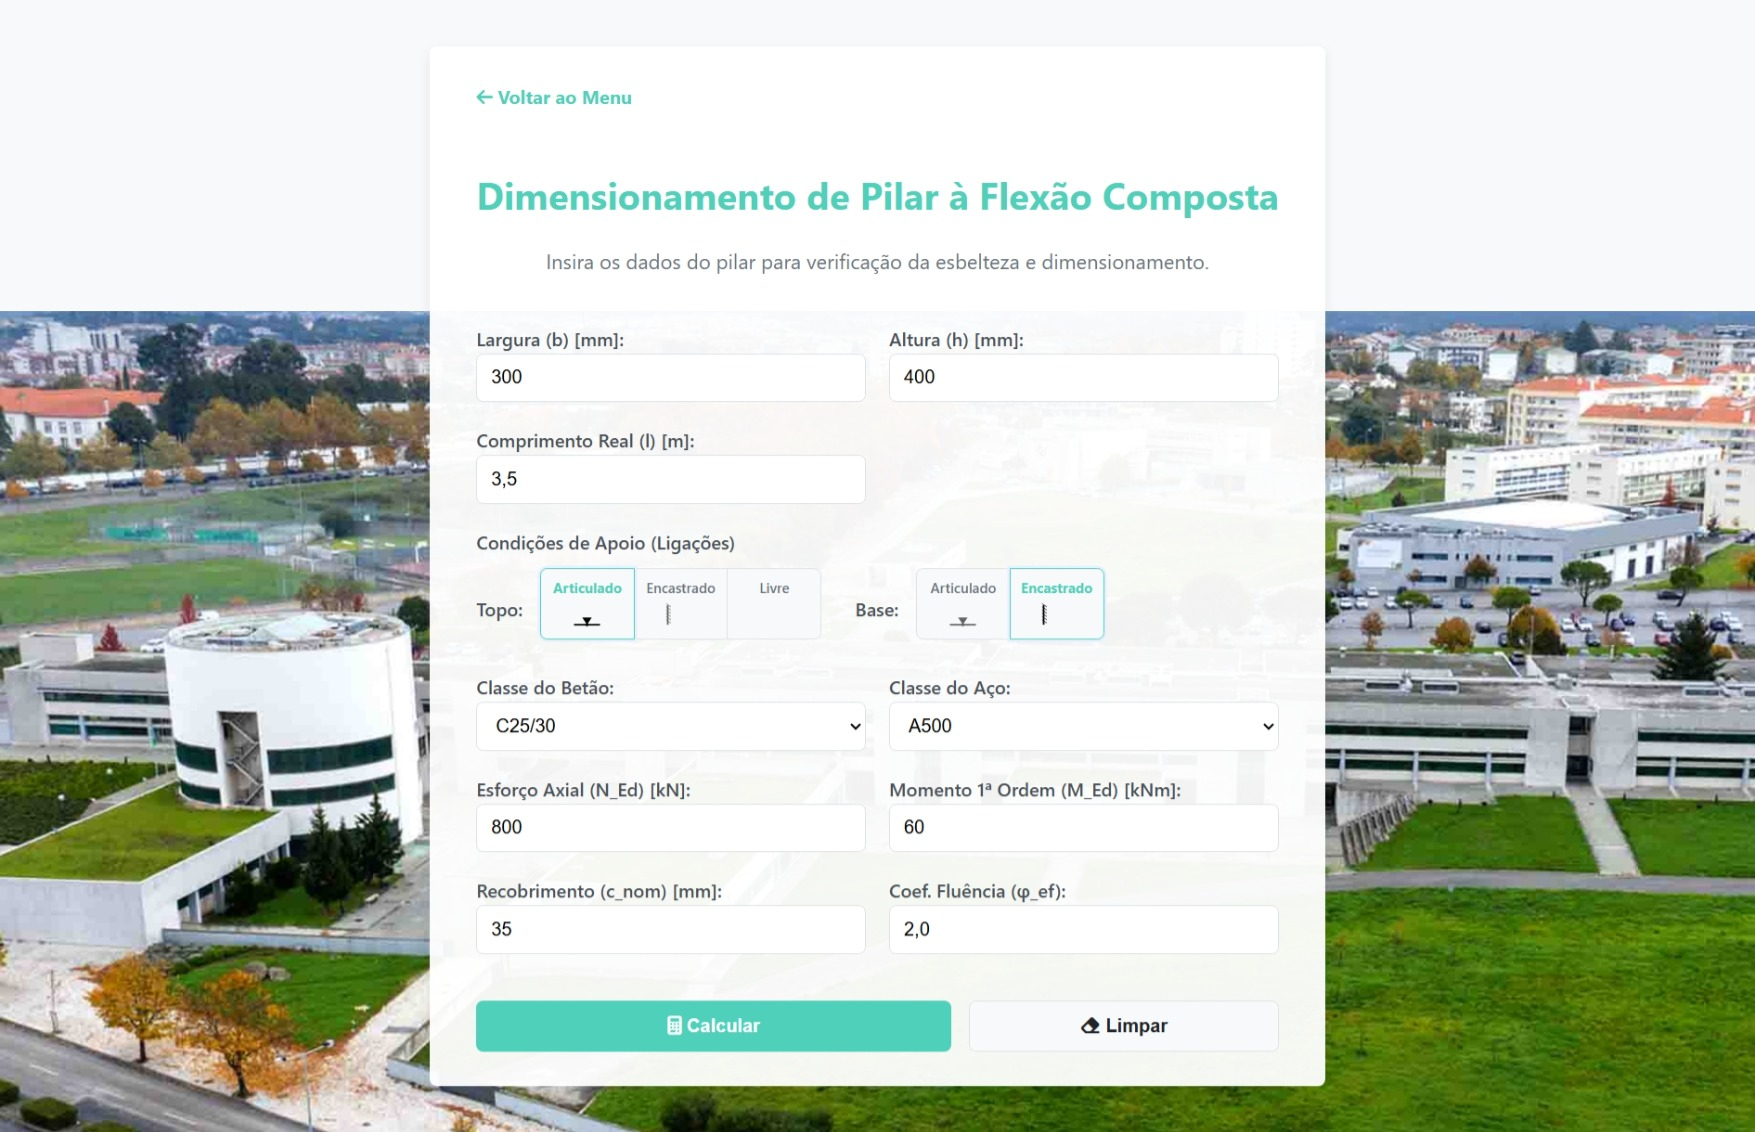
\includegraphics[width=0.88\textwidth]{Figuras/Pilar.jpg}}
    \caption{Formulário de entrada de dados para o dimensionamento de elementos do tipo pilar, com seleção visual das condições de apoio.}
    \label{fig:pilar_input}
\end{figure}

\paragraph{Visualização de Resultados}
O sistema apresenta a verificação de instabilidade e a armadura simétrica calculada. O desenho gerado ilustra a distribuição dos varões nas quatro faces. A interface de resultados pode ser consultada no no apêndice J.

\subsubsection{Módulo de Sapatas}

\paragraph{Entrada de Dados}
O utilizador introduz a tensão admissível do solo ($\sigma_{adm}$), as dimensões do pilar e os esforços atuantes ($N_{Ed}, M_{Ed}$).

\begin{figure}[htbp]
    \centering
    {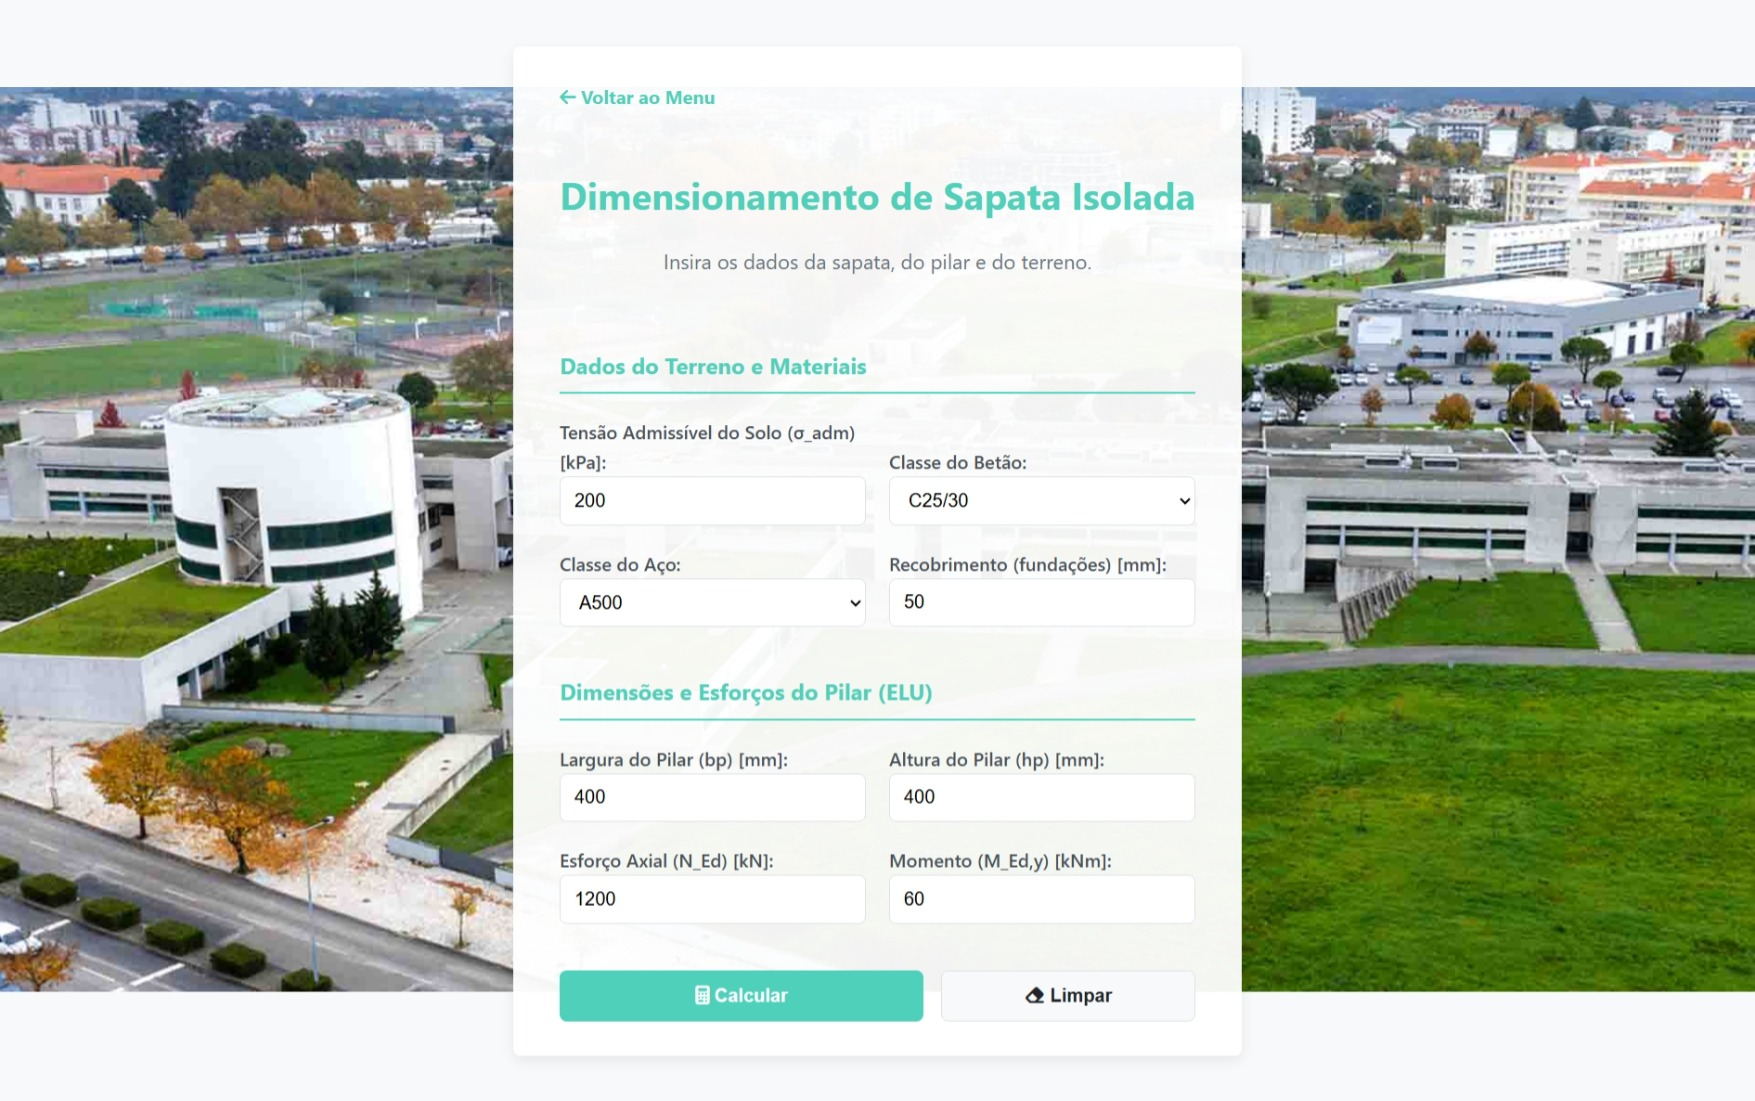
\includegraphics[width=0.9\textwidth]{Figuras/Sapata.jpg}}
    \caption{Formulário de entrada de dados para o dimensionamento de elementos do de sapata isolada.}
    \label{fig:sapata_input}
\end{figure}

\paragraph{Visualização de Resultados}


O resultado final inclui as dimensões em planta otimizadas e a altura verificada ao punçoamento, acompanhadas pelas vistas em planta e corte. A interface completa com estes resultados é apresentada no apêndice K.

\subsubsection{Ferramentas de Gestão}

\paragraph{Histórico de Cálculos}

Todos os dimensionamentos são guardados na base de dados. A tabela de histórico permite consultar e recuperar cálculos anteriores com interface completa
disponível no Apêndice G.

\paragraph{Configuração do Sistema}

O painel de configuração permite ao utilizador personalizar o aspeto visual da aplicação, alternando temas e cores, conforme ilustrado no Apêndice H.

\subsection{Disponibilização da aplicação}

A aplicação desenvolvida encontra-se disponibilizada em ambiente web na plataforma PythonAnywhere \cite{PythonAnywhere}, um serviço online de alojamento e execução de aplicações Python que permite publicar aplicações web na cloud. A versão funcional do sistema pode ser acedida online \cite{AppWeb_Tese}.
Paralelamente, o código-fonte da aplicação e dos algoritmos de dimensionamento encontra-se versionado no repositório GitHub \cite{RepoGitHub_Tese}. Esta separação entre ambiente de execução e repositório de código contribui para a organização do projeto, para a manutenção futura da aplicação e para a rastreabilidade das alterações efetuadas ao longo do desenvolvimento.


\subsection{Integração com análise matricial (Structrun)}

A aplicação está preparada para integração bidirecional com o Structrun \cite{Structrun} via JSON:

\begin{enumerate}
\item \textbf{Input}: gera \texttt{input.json} com geometria/nós/elementos.
\item \textbf{Processo}: invoca Structrun como subprocesso.
\item \textbf{Output}: lê \texttt{results.json} → alimenta automaticamente $N_\text{Ed}$, $M_\text{Ed}$.
\end{enumerate}

Esta cadeia completa (análise → dimensionamento) constitui perspetiva de evolução futura.

% Capítulo 6
\newpage
\section{TESTES E VALIDAÇÕES DA APLICAÇÃO}
\subsection{Introdução}

A validação da aplicação desenvolvida constitui uma etapa essencial para demonstrar a fiabilidade dos algoritmos de dimensionamento implementados para vigas, pilares e sapatas isoladas segundo Eurocódigo EC2 A formulação teórica dos modelos de cálculo e dos critérios normativos foi previamente estabelecida nos Capítulos 3 e 4, pelo que o presente capítulo se centra na verificação prática das entradas, do processamento interno e das saídas produzidas pela aplicação.

A estratégia adotada combina dois níveis complementares de validação. Por um lado, recorrem-se a casos de teste automatizados, integrados no ambiente de desenvolvimento, com o objetivo de garantir a consistência do código ao longo da evolução do sistema. Por outro lado, procede-se à comparação detalhada entre os resultados da aplicação e exemplos resolvidos de obras de referência, designadamente Goodchild et al. \cite{Goodchild} e Mosley et al. \cite{Mosley}, permitindo aferir a coerência estrutural e normativa dos resultados obtidos.

\subsection{Metodologia de Teste}

A validação computacional foi estruturada com base em testes unitários automatizados, implementados no ambiente Django. Esta abordagem permite verificar, de forma repetível e objetiva, se as funções responsáveis pelo dimensionamento dos diferentes elementos retornam resultados compatíveis com os valores esperados para um conjunto conhecido de dados de entrada.

Cada teste define previamente a geometria, os materiais, os carregamentos e os parâmetros regulamentares do elemento estrutural a analisar, executando depois o serviço de cálculo correspondente. Os resultados produzidos são comparados com valores de referência, obtidos por resolução manual ou extraídos de exemplos académicos reconhecidos. Deste modo, assegura-se não apenas a correção matemática das rotinas implementadas, mas também a sua estabilidade perante futuras alterações ao código.

Para complementar esta verificação automática, foram selecionados três casos de estudo representativos: um caso de dimensionamento à flexão simples de uma viga, um caso de dimensionamento de um pilar sujeito a flexão composta com verificação de esbelteza, e um caso de dimensionamento de uma sapata isolada sujeita a carga centrada. Estes três exemplos permitem cobrir diferentes mecanismos resistentes e diferentes tipos de verificação previstos no Eurocódigo 2.

\subsection{Casos de Teste e Resultados}

\subsubsection{Validação da viga}

A validação do módulo de vigas foi realizada com base num caso de flexão simples em secção retangular, comparando a solução produzida pela aplicação com a resolução de referência apresentada por Goodchild et al. \cite{Goodchild} e com o relatório interno da aplicação. O objetivo principal desta validação é confirmar a correção do cálculo da altura útil, do momento reduzido, da área de armadura necessária e da solução construtiva final adotada.

\paragraph{Enunciado do caso de validação}

Considere-se a secção de apoio intermédio de uma viga contínua de betão armado, de secção retangular com largura \(b = 300\ \text{mm}\) e altura total \(h = 450\ \text{mm}\). O momento fletor de cálculo atuante é \(M_{Ed} = 193.8\ \text{kNm}\). Os materiais adotados são betão C30/37 \((f_{ck}=30\ \text{MPa})\), aço A500 \((f_{yk}=500\ \text{MPa})\) e recobrimento nominal \(c_{nom}=35\ \text{mm}\). A Figura~\ref{fig:viga_validacao} apresenta a geometria simplificada da secção analisada.

\begin{figure}[H]
\centering
\begin{tikzpicture}[>=Stealth, scale=1.0]
\draw[thick, fill=gray!15] (0,0) rectangle (3,4.5);
\draw[<->] (0,-0.5) -- (3,-0.5) node[midway, below] {$300\ \text{mm}$};
\draw[<->] (-0.5,0) -- (-0.5,4.5) node[midway, left] {$450\ \text{mm}$};
\end{tikzpicture}
\caption{Secção transversal da viga considerada na validação.}
\label{fig:viga_validacao}
\end{figure}

\paragraph{Resolução segundo Goodchild et al.}

Segundo o Exemplo 4.1 de Goodchild et al.~\cite{Goodchild}, o procedimento manual recorre inicialmente a simplificações para avaliar as dimensões exigidas:

Altura útil é inicialmente estimada admitindo estribos de \(10\ \text{mm}\) e armadura longitudinal de \(25\ \text{mm}\), obtendo-se:
\begin{equation}
d = 450 - 35 - 10 - \frac{25}{2} = 392\ \text{mm}
\end{equation}

O coeficiente reduzido de momento resulta:
\begin{equation}
K = \frac{M_{Ed}}{b d^2 f_{ck}}
= \frac{193.8 \times 10^6}{300 \times 392^2 \times 30}
= 0.142
\end{equation}

Como o valor calculado se mantém dentro do domínio de flexão simples, a secção pode ser tratada sem necessidade de armadura de compressão. Admitindo um braço interno aproximado \(z \approx 0.864d\), obtém-se:
\begin{equation}
z \approx 0.864 \times 392 = 338\ \text{mm}
\end{equation}

A área de armadura necessária é:
\begin{equation}
A_{s,req} =
\frac{M_{Ed}}{f_{yd} z}
=
\frac{193.8 \times 10^6}{(500/1.15)\times 338}
= 1319\ \text{mm}^2
= 13.19\ \text{cm}^2
\end{equation}

Garantindo a verificação das disposições mínimas do Eurocódigo, resulta:
\begin{equation}
    A_{s,min} = \max\left[ 0{,}26 \left( \frac{f_{ctm}}{f_{yk}} \right) b_t \cdot d;\, 0{,}0013 \cdot b_t \cdot d \right] = 177\ \text{mm}^2 = 1{,}77\ \text{cm}^2
\end{equation}

A solução adotada na referência é \(3\phi25\), correspondente a \(14.73\ \text{cm}^2\), valor superior ao requerido.

\paragraph{Resolução pela aplicação desenvolvida}

Na aplicação, o cálculo é realizado de forma iterativa. Numa primeira iteração, assume-se \(\phi_{est}=8\ \text{mm}\) para os estribos e \(\phi_{long}=16\ \text{mm}\), resultando:
\begin{equation}
d_1 = 450 - 35 - 8 - \frac{16}{2} = 399.0\ \text{mm}
\end{equation}

Com este valor, o memento reduzido inicial é:
\begin{equation}
\mu_1 =
\frac{193800}{0.3 \times 0.399^2 \times 20\times 10^6}
= 0.203
\end{equation}

Como a solução de varão único apontada na primeira aproximação difere do diâmetro inicialmente assumido, o algoritmo executa uma segunda iteração com \(\phi = 25\ \text{mm}\), recalculando a altura útil:
\begin{equation}
d_2 = 450 - 35 - 8 - \frac{25}{2} = 394.5\ \text{mm}
\end{equation}

O momento reduzido final passa a:
\begin{equation}
\mu_2 =
\frac{193800}{0.3 \times 0.395^2 \times 20\times 10^6}
= 0.208
\end{equation}

Com base neste valor, a aplicação determina:
\begin{equation}
\xi = \frac{1-\sqrt{1-2\mu}}{0.8} = 0.294
\end{equation}
\begin{equation}
z = d(1-0.5\times 0.8 \times 0.294) = 0.348\ \text{m}
\end{equation}
\begin{equation}
A_{s,req} =
\frac{193800}{0.348 \times 434.78\times 10^6}
= 12.80\ \text{cm}^2
\end{equation}

A solução final mais económica encontrada pelo algoritmo é:
\begin{equation}
2\phi10 + 4\phi20
\end{equation}
com área total:
\begin{equation}
A_{s,prov} = 14.14\ \text{cm}^2
\end{equation}

A armadura mínima calculada pela aplicação é \(1.78\ \text{cm}^2\), pelo que a solução adotada satisfaz confortavelmente a exigência regulamentar. Além disso, a aplicação acrescenta uma armadura superior construtiva \(2\phi10\), destinada ao apoio e amarração dos estribos, sem participação no momento resistente principal.

\begin{table}[H]
\centering
\caption{Comparação entre a referência e a aplicação para a viga.}
\label{tab:comp_viga}
\renewcommand{\arraystretch}{1.2}
\begin{tabular}{lcc}
\toprule
\textbf{Parâmetro} & \textbf{Goodchild et al.} & \textbf{Aplicação} \\
\midrule
Secção [mm] & \(300 \times 450\) & \(300 \times 450\) \\
\(M_{Ed}\) [kNm] & 193.8 & 193.8 \\
Altura útil \(d\) [mm] & 392 & 394.5 \\
Momento reduzido & 0.142 & 0.208 \\
\(A_{s,req}\) [cm\(^2\)] & 13.19 & 12.80 \\
Armadura adotada & \(3\phi25\) & \(2\phi10 + 4\phi20\) \\
\(A_{s,prov}\) [cm\(^2\)] & 14.73 & 14.14 \\
\bottomrule
\end{tabular}
\end{table}

\paragraph{Comparação dos resultados}
Os resultados revelam uma concordância muito satisfatória entre ambas as abordagens. A diferença principal resulta do facto de a aplicação recalcular explicitamente a altura útil e o braço mecânico com base na solução efetivamente adotada, enquanto a resolução de referência usa simplificações de pré-dimensionamento mais diretas.
Ainda assim, a área de armadura final obtida pela aplicação mantém-se muito próxima da referência e confirma a consistência do algoritmo implementado.

\subsubsection{Validação do pilar}

A validação do módulo de pilares foi realizada com base no Exemplo 5.1 de Goodchild et al. \cite{Goodchild}, correspondente a um pilar de bordo sujeito a esforço axial elevado e momentos de extremidade opostos. Este caso é particularmente relevante porque permite testar a verificação de esbelteza, a consideração dos efeitos de segunda ordem e o dimensionamento da armadura longitudinal em flexão composta reta.

\paragraph{Enunciado do caso de validação}

Considere-se um pilar com secção quadrada \(300 \times 300\ \text{mm}\), comprimento real \(l = 3.75\ \text{m}\), ligação encastrada no topo e articulada na base. O esforço axial de cálculo é \(N_{Ed}=1620\ \text{kN}\) e o momento fletor de primeira ordem considerado na aplicação é \(M_{0Ed}=51.4\ \text{kNm}\). Os materiais adotados são betão C30/37 \((f_{ck}=30\ \text{MPa})\), aço A500 \((f_{yk}=500\ \text{MPa})\) e recobrimento nominal \(c_{nom}=25\ \text{mm}\). A Figura~\ref{fig:pilar_validacao} representa o esquema simplificado do elemento.

\begin{figure}[H]
\centering
\begin{tikzpicture}[>=Stealth, scale=1.0]
\draw[thick] (0,0) rectangle (1.5,6);
\draw[thick] (-0.5,6) -- (2.0,6);
\draw[thick] (0.75,0) circle (0.12);
\draw[->, ultra thick] (0.75,7.2) -- (0.75,6.2);
\draw[->, thick] (1.4, 6.5) arc (0:180:0.65);
\node at (2.6, 7.0) {$M_{0Ed} = 51.4\ \text{kNm}$};
\draw[<->] (-1.5,0) -- (-1.5,6) node[midway, left] {$3.75\ \text{m}$};
\node at (0.75,7.5) {$N_{Ed} = 1620\ \text{kN}$};
\node at (3.4,5.2) {Topo: encastrado};
\node at (3.2,0.4) {Base: articulada};
\node at (0.75,-0.5) {$300\ \text{mm}$};
\end{tikzpicture}
\caption{Esquema do pilar considerado na validação.}
\label{fig:pilar_validacao}
\end{figure}

\paragraph{Resolução segundo Goodchild et al.}

No exemplo de referência, o fator de comprimento eficaz é \(\beta = 0.85\), pelo que:
\begin{equation}
l_0 = \beta \cdot l = 0.85 \times 3750 = 3187.5\ \text{mm}
\end{equation}

O raio de giração para a secção quadrada é:
\begin{equation}
i = \frac{h}{\sqrt{12}} = \frac{300}{\sqrt{12}} = 86.6\ \text{mm}
\end{equation}

A esbelteza resulta:
\begin{equation}
\lambda = \frac{l_0}{i} = \frac{3187.5}{86.6} = 36.8
\end{equation}

Segundo a formulação adotada por Goodchild et al., com \(A=0.7\), \(B=1.1\), \(C=2.7\) e \(n=1.06\), a esbelteza limite é:
\begin{equation}
\lambda_{lim}= \frac{20 \cdot A \cdot B \cdot C}{\sqrt{n}} = \frac{20 \cdot 0.7 \cdot 1.1 \cdot 2.7}{\sqrt{1.06}} = 40.4
\end{equation}

Como \(\lambda < \lambda_{lim}\), o pilar é classificado como não esbelto na referência, pelo que não são considerados efeitos adicionais de segunda ordem. O momento de dimensionamento permanece \(M_{Ed} = 51.4\ \text{kNm}\) e a armadura longitudinal adotada na referência é \(4H25\), correspondente a \(A_{s} = 1964\ \text{mm}^2 = 19.64\ \text{cm}^2\).

\paragraph{Resolução pela aplicação}

Na aplicação, o fator de comprimento eficaz é igualmente \(\beta=0.85\), pelo que:
\begin{equation}
l_0 = 0.85 \times 3.75 = 3.188\ \text{m}
\end{equation}

As resistências de cálculo são:
\begin{equation}
f_{cd} = \frac{30}{1.5} = 20.00\ \text{MPa}
\end{equation}
\begin{equation}
f_{yd} = \frac{500}{1.15} = 434.78\ \text{MPa}
\end{equation}

O valor de esbelteza é:
\begin{equation}
\lambda = \frac{3188}{86.6} = 36.81
\end{equation}

A aplicação usa:
\begin{equation}
n = \frac{N_{Ed}}{A_c f_{cd}} = 0.900
\end{equation}
\begin{equation}
A = 1.0,\quad B = 1.1,\quad C = 0.7
\end{equation}

Logo:
\begin{equation}
\lambda_{lim} = \frac{20 \cdot A \cdot B \cdot C}{\sqrt{n}} = 16.23
\end{equation}

Como \(\lambda = 36.81 > 16.23\), a aplicação classifica o elemento como esbelto e ativa o cálculo de segunda ordem pelo método da curvatura nominal.

A curvatura inicial é:
\begin{equation}
\frac{1}{r_0} = \frac{\varepsilon_{yd}}{0.45d} = 0.00001865\ \text{mm}^{-1}
\end{equation}

Com \(\omega \approx 0.090\), \(K_r=0.275\), \(\beta=0.255\) e \(K_\phi=1.000\), resulta:
\begin{equation}
\frac{1}{r} = 0.275 \times 1.000 \times 0.00001865 = 0.00000514\ \text{mm}^{-1}
\end{equation}

A excentricidade de segunda ordem é:
\begin{equation}
e_2 = \frac{1}{r}\frac{l_0^2}{10} = 5.2\ \text{mm}
\end{equation}

O momento adicional é:
\begin{equation}
M_2 = N_{Ed}\times e_2 = 1620 \times 0.0052 = 8.45\ \text{kNm}
\end{equation}

Assim, o momento total de dimensionamento torna-se:
\begin{equation}
M_{Ed,total} = 51.40 + 8.45 = 59.85\ \text{kNm}
\end{equation}

Quanto à armadura, a aplicação calcula:
\begin{equation}
A_{s,min} = \max\left(0.10\frac{N_{Ed}}{f_{yd}},\ 0.002A_c\right)=3.73\ \text{cm}^2
\end{equation}
\begin{equation}
A_{s,req} = 7.75\ \text{cm}^2
\end{equation}
\begin{equation}
A_{s,max}=36.00\ \text{cm}^2
\end{equation}

A solução construtiva ótima é:
\begin{equation}
4\phi16
\end{equation}
com área fornecida:
\begin{equation}
A_{s,prov} = 8.04\ \text{cm}^2
\end{equation}

\begin{table}[H]
\centering
\caption{Comparação entre a referência e a aplicação para o pilar.}
\label{tab:comp_pilar}
\renewcommand{\arraystretch}{1.2}
\begin{tabular}{lcc}
\toprule
\textbf{Parâmetro} & \textbf{Goodchild et al.} & \textbf{Aplicação} \\
\midrule
Secção [mm] & \(300 \times 300\) & \(300 \times 300\) \\
\(M_{Ed}\) [kNm] & 51.4 & 51.4 \\
\(V_{Ed}\) [kNm] & 1620 & 1620 \\
Comprimento eficaz \(l_0\) [m] & 3.1875 & 3.19 \\
Esbelteza \(\lambda\) & 36.8 & 36.81 \\
Esbelteza limite \(\lambda_{lim}\) & 40.4 & 16.23 \\
Classificação & Não esbelto & Esbelto \\
Momento de cálculo [kNm] & 51.4 & 59.85 \\
Armadura adotada & \(4H25\) & \(4\phi16\) \\
Área de aço [cm\(^2\)] & 19.64 & 8.04 \\
\bottomrule
\end{tabular}
\end{table}

\paragraph{Comparação dos resultados}
As diferenças observadas decorrem essencialmente dos parâmetros normativos adotados. Enquanto a referência segue o enquadramento do Anexo Nacional britânico, com \(\alpha_{cc}=0.85\) e um valor elevado de \(C\) para dupla curvatura, a aplicação usa diretamente os valores base do EC2, com \(\alpha_{cc}=1.0\) e \(C=0.7\), conduzindo a uma verificação mais conservadora da esbelteza. Ainda assim, o comportamento global do algoritmo é coerente, e o caso comprova que a aplicação trata corretamente a transição entre pilares não esbeltos e pilares esbeltos, bem como o cálculo dos efeitos de segunda ordem.

\subsubsection{Validação da sapata}

A validação do módulo de sapatas isoladas foi realizada com base no Exemplo 10.1 de Mosley et al \cite{Mosley}, correspondente ao dimensionamento de uma sapata centrada para um pilar quadrado. Este caso permite avaliar a coerência do algoritmo em três etapas fundamentais: o dimensionamento geotécnico em serviço, a verificação ao punçoamento em estado limite último e o dimensionamento da armadura inferior de flexão.

\paragraph{Enunciado do caso de validação}

Considere-se uma sapata isolada que suporta um pilar quadrado com secção \(400 \times 400\ \text{mm}\). As ações características aplicadas são \(G_k = 1000\ \text{kN}\) e \(Q_k = 350\ \text{kN}\). A tensão admissível do terreno é \(\sigma_{adm}=200\ \text{kN/m}^2\). Os materiais considerados são betão C30/37 \((f_{ck}=30\ \text{MPa})\), aço A500 \((f_{yk}=500\ \text{MPa})\) e recobrimento nominal \(c_{nom}=50\ \text{mm}\). A Figura~\ref{fig:sapata_validacao_enunciado} apresenta a geometria base do caso de estudo.

\begin{figure}[H]
\centering
\begin{tikzpicture}[scale=1.1, >=Stealth]
\draw[thick] (0,0) rectangle (5,5);
\draw[thick, fill=gray!20] (2.143,2.143) rectangle (2.857,2.857);
\draw[<->] (0,-0.5) -- (5,-0.5) node[midway, below] {$2.80\ \text{m}$};
\draw[<->] (-0.5,0) -- (-0.5,5) node[midway, left] {$2.80\ \text{m}$};
\draw[<->] (2.143,3.1) -- (2.857,3.1) node[midway, above] {$400\ \text{mm}$};
\draw[dashed] (2.143,2.857) -- (2.143,3.2);
\draw[dashed] (2.857,2.857) -- (2.857,3.2);
\draw[dashed] (2.857,2.857) -- (3.3,2.857);
\draw[dashed] (2.857,2.143) -- (3.3,2.143);
\draw[<->] (3.1,2.143) -- (3.1,2.857) node[midway, right] {$400\ \text{mm}$};
\node[align=left] at (7.1,4.4) {$G_k = 1000\ \text{kN}$};
\node[align=left] at (7.1,3.8) {$Q_k = 350\ \text{kN}$};
\node[align=left] at (7.4,3.2) {$\sigma_{adm} = 200\ \text{kN/m}^2$};
\node[align=left] at (7.0,2.6) {$f_{ck} = 30\ \text{MPa}$};
\node[align=left] at (7.0,2.0) {$f_{yk} = 500\ \text{MPa}$};
\end{tikzpicture}
\caption{Geometria e dados de partida da sapata isolada de validação.}
\label{fig:sapata_validacao_enunciado}
\end{figure}

\paragraph{Resolução segundo Mosley et al.}

Na verificação em estado limite de utilização, Mosley et al. consideram um peso próprio aproximado da sapata de \(150\ \text{kN}\), pelo que a carga total de serviço é:
\begin{equation}
N_{ser}=1150+350=1500\ \text{kN}
\end{equation}

A área mínima necessária da base é:
\begin{equation}
A_{req}=\frac{1500}{200}=7.50\ \text{m}^2
\end{equation}

Adota-se uma sapata quadrada com:
\begin{equation}
A=B=2.80\ \text{m}
\end{equation}
e área:
\begin{equation}
A_{base}=2.80\times 2.80 = 7.84\ \text{m}^2
\end{equation}

Em estado limite último, a carga de cálculo é:
\begin{equation}
N_{Ed}=1.35\times 1000 + 1.5\times 350 = 1875\ \text{kN}
\end{equation}

A tensão média no terreno é:
\begin{equation}
\sigma_{Ed}=\frac{1875}{2.8^2}=239\ \text{kN/m}^2
\end{equation}

Adotando \(H=600\ \text{mm}\) e altura útil média \(d=520\ \text{mm}\), o punçoamento é verificado no perímetro de controlo:
\begin{equation}
u_1 = 4\times 400 + 4\pi\times 520 = 8134\ \text{mm}
\end{equation}

A força de punçoamento é:
\begin{equation}
V_{Ed}=239(2.8^2-5.22)=626\ \text{kN}
\end{equation}

A armadura de flexão é calculada a partir do momento crítico na face do pilar:
\begin{equation}
M_{Ed}=(239\times 2.8 \times 1.2)\times \frac{1.2}{2}=482\ \text{kNm}
\end{equation}

A área requerida é:
\begin{equation}
A_s=\frac{482\times 10^6}{0.87\times 500 \times (0.95\times 520)} = 2243\ \text{mm}^2
\end{equation}

A solução adotada por Mosley et al. é:
\begin{equation}
12\phi16 @ 225\ \text{mm\ e.w.}
\end{equation}
com área fornecida \(A_{s,prov}=2412\ \text{mm}^2\). Na verificação final, a resistência ao punçoamento sem armadura transversal é:
\begin{equation}
V_{Rd,c}=1691\ \text{kN}
\end{equation}
pelo que a solução é considerada segura.

\paragraph{Resolução pela aplicação desenvolvida}

Na aplicação, o processo é iterativo e organizado em três fases. Na fase geotécnica, parte-se da carga de serviço equivalente:
\begin{equation}
N_k \approx \frac{1875}{1.4}=1339.29\ \text{kN}
\end{equation}

A área teórica necessária é:
\begin{equation}
A_{req}=\frac{1339.29}{200}=6.70\ \text{m}^2
\end{equation}

Para incorporar de forma simplificada o peso próprio e efeitos adicionais, a aplicação majora esta área em 20\%:
\begin{equation}
A_{maj}=1.20\times 6.70=8.04\ \text{m}^2
\end{equation}

Sendo o pilar quadrado, assume-se inicialmente uma sapata quadrada:
\begin{equation}
A=B=\sqrt{8.04}=2.83\ \text{m}
\end{equation}

Na iteração geotécnica, com altura estimada \(H_{est}=0.40\ \text{m}\), o peso próprio é:
\begin{equation}
W_k = 2.83\times 2.83\times 0.40\times 25=80.36\ \text{kN}
\end{equation}

A carga total de serviço é:
\begin{equation}
N_{total,k}=1339.29+80.36=1419.64\ \text{kN}
\end{equation}

Sem excentricidade, as tensões extremas no terreno coincidem:
\begin{equation}
\sigma_{max}=\sigma_{min}=176.67\ \text{kPa}
\end{equation}

Como este valor é inferior à tensão admissível, a aplicação arredonda as dimensões finais para:
\begin{equation}
A=B=2.85\ \text{m}
\end{equation}

Em estado limite último:
\begin{equation}
f_{cd}=\frac{30}{1.5}=20.00\ \text{MPa}
\end{equation}
\begin{equation}
f_{yd}=\frac{500}{1.15}=434.78\ \text{MPa}
\end{equation}
\begin{equation}
\sigma_{Ed}=\frac{1875}{2.85\times 2.85}=230.84\ \text{kN/m}^2
\end{equation}

Na verificação ao punçoamento, a aplicação encontra iterativamente como primeiro valor satisfatório:
\begin{equation}
d=480\ \text{mm}
\end{equation}

Para este valor:
\begin{equation}
u_1 = 2(400+400)+2\pi(480)=4616\ \text{mm}
\end{equation}
\begin{equation}
A_{crit}=(0.400+\pi\times 0.480)^2=3.64\ \text{m}^2
\end{equation}
\begin{equation}
k=1+\sqrt{\frac{200}{480}}=1.645
\end{equation}
\begin{equation}
V_{Ed}=1875 - 230.84\times 3.64=1034.67\ \text{kN}
\end{equation}
\begin{equation}
V_{Rd,c}=1078.97\ \text{kN}
\end{equation}

Como \(V_{Ed}\leq V_{Rd,c}\), a altura útil é aceite. A altura total resulta:
\begin{equation}
H \approx 480+50+\frac{16}{2}=538\ \text{mm}
\end{equation}
sendo arredondada para:
\begin{equation}
H = 550\ \text{mm}
\end{equation}

No dimensionamento à flexão, como a sapata é quadrada e o carregamento é centrado, os voos são iguais:
\begin{equation}
l_x=l_y=\frac{2.85-0.40}{2}=1.225\ \text{m}
\end{equation}

O momento por metro em cada direção é:
\begin{equation}
M_{Ed,x}=M_{Ed,y}=\frac{230.84\times 1.225^2}{2}=173.20\ \text{kNm/m}
\end{equation}

A armadura necessária é:
\begin{equation}
A_{s,x,req}=8.92\ \text{cm}^2/\text{m}
\end{equation}
\begin{equation}
A_{s,y,req}=9.07\ \text{cm}^2/\text{m}
\end{equation}

A armadura mínima calculada é:
\begin{equation}
A_{s,min}=7.47\ \text{cm}^2/\text{m}
\end{equation}

A aplicação adota então uma malha única em ambas as direções:
\begin{equation}
13\phi16 \ \text{em X e Y}
\end{equation}
com:
\begin{equation}
A_{s,prov,total}=13\times 2.01 = 26.14\ \text{cm}^2
\end{equation}
e área distribuída:
\begin{equation}
A_{s,prov}= \frac{26.14}{2.85}=9.17\ \text{cm}^2/\text{m}
\end{equation}
correspondendo a espaçamento real aproximado:
\begin{equation}
s \approx 228\ \text{mm}
\end{equation}

\begin{figure}[H]
    \centering
    \begin{tikzpicture}[>=latex, scale=2.3]
        \path[use as bounding box] (-1.5, -1.2) rectangle (4.5, 3.5);
        \draw[thick] (0,0) rectangle (2.85, 2.85);
        \draw[thick, fill=gray!30] (1.225, 1.225) rectangle (1.625, 1.625);
        \foreach \x in {0.2, 0.404, 0.608, 0.812, 1.016, 1.22, 1.425, 1.63, 1.834, 2.038, 2.242, 2.446, 2.65} {
            \draw[blue!60, very thin] (\x, 0.1) -- (\x, 2.75);
            \draw[red!60, very thin] (0.1, \x) -- (2.75, \x);
        }
        \node[rotate=90, text=blue!80!black] at (-0.8, 1.425) {\small Dir Y: 13$\varnothing$16};
        \node[text=red!80!black] at (1.425, -0.8) {\small Dir X: 13$\varnothing$16};
        \draw[|<->|] (0, 3.1) -- (2.85, 3.1) node[midway, above] {\small $2{,}85\ \text{m}$};
        \draw[|<->|] (3.1, 0) -- (3.1, 2.85) node[midway, right] {\small $2{,}85\ \text{m}$};
    \end{tikzpicture}
    
    \vspace{0.2cm}
    \centerline{(a) Planta}
\end{figure}

%\newpage

\begin{figure}[H]
    \centering
    \begin{tikzpicture}[>=latex, scale=2.3]
        \path[use as bounding box] (-1.5, -1.6) rectangle (4.5, 2.1);
        \draw[thick] (0, 0) -- (2.85, 0) -- (2.85, 0.55) -- (0, 0.55) -- cycle;
        \draw[thick, fill=gray!30] (1.225, 0.55) rectangle (1.625, 1.5);
        \draw[thick] (1.1, 1.4) -- (1.75, 1.4); 
        \draw[thick, red] (0.1, 0.08) -- (2.75, 0.08);
        \foreach \x in {0.2, 0.404, 0.608, 0.812, 1.016, 1.22, 1.425, 1.63, 1.834, 2.038, 2.242, 2.446, 2.65} {
            \filldraw[blue] (\x, 0.14) circle (1.5pt);
        }
        \draw[|<->|] (-0.5, 0) -- (-0.5, 0.55) node[midway, left] {\small $550\ \text{mm}$};
        \draw[|<->|] (1.225, 1.7) -- (1.625, 1.7) node[midway, above] {\small $400\ \text{mm}$};
        \draw[|<->|] (0, -0.6) -- (2.85, -0.6) node[midway, below] {\small $2{,}85\ \text{m}$};
        \node at (1.425, -1.2) {\small Espaçamento real: $s \approx 228\ \text{mm}$};
    \end{tikzpicture}
    
    \vspace{0.2cm}
    \centerline{(b) Corte A-A}
    
    \vspace{0.6cm}
    \caption{Sapata dimensionada pela aplicação: (a) planta de armaduras e (b) corte transversal.}
    \label{fig:sapata_aplicacao}
\end{figure}

\begin{table}[H]
\centering
\caption{Comparação entre referência e a aplicação para a sapata isolada.}
\label{tab:comp_sapata}
\renewcommand{\arraystretch}{1.2}
\begin{tabular}{lcc}
\toprule
\textbf{Parâmetro} & \textbf{Mosley et al.} & \textbf{Aplicação} \\
\midrule
Dimensões \(A\times B\) [m] & \(2.80\times 2.80\) & \(2.85\times 2.85\) \\
Espessura \(H\) [m] & 0.60 & 0.55 \\
Área da base [m\(^2\)] & 7.84 & 8.12 \\
\(\sigma_{Ed}\) [kN/m\(^2\)] & 239.00 & 230.84 \\
Altura útil \(d\) [mm] & 520 & 480 \\
\(V_{Ed}\) punçoamento [kN] & 626 & 1034.67 \\
\(V_{Rd,c}\) [kN] & 1691 & 1078.97 \\
Armadura requerida & \(2243\ \text{mm}^2\) & \(9.07\ \text{cm}^2/\text{m}\) \\
Armadura adotada & \(12\phi16 @ 225\ \text{mm}\) & \(13\phi16\), \(s\approx 228\ \text{mm}\) \\
\bottomrule
\end{tabular}
\end{table}

\paragraph{Comparação dos resultados}

As duas soluções são estruturalmente coerentes e da mesma ordem de grandeza. A aplicação conduz a uma base ligeiramente maior em planta, mas a uma espessura total inferior, refletindo a natureza iterativa do algoritmo e a forma própria como este trata a verificação geotécnica, a estimativa do peso próprio e a procura do primeiro valor satisfatório de altura útil ao punçoamento. Apesar dessas diferenças, a solução final mantém margens de segurança adequadas e confirma a robustez do módulo desenvolvido.

\subsection{Conclusão da Validação}

A análise dos três casos de estudo confirma a consistência global da aplicação desenvolvida para o dimensionamento de vigas, pilares e sapatas isoladas segundo o Eurocódigo 2. Em todos os casos, os resultados obtidos revelaram concordância satisfatória com exemplos de referência da literatura, demonstrando que os algoritmos implementados reproduzem de forma coerente os principais procedimentos de cálculo, verificação e seleção construtiva da armadura.

No caso das vigas, a comparação com Goodchild et al. mostrou que a aplicação conduz a resultados muito próximos da resolução de referência, embora recorra a um procedimento mais rigoroso no recálculo da altura útil e do braço mecânico, com base na solução efetivamente adotada. Esta diferença metodológica traduz-se numa ligeira variação da área de armadura requerida, mas não compromete a coerência resistente nem a conformidade regulamentar da solução final.

Na validação do pilar, verificou-se igualmente boa concordância na definição geométrica, no comprimento eficaz e no cálculo da esbelteza. As diferenças observadas na classificação do elemento como esbelto ou não esbelto resultam essencialmente da adoção de parâmetros normativos distintos entre a referência bibliográfica e a aplicação, nomeadamente no valor de $\alpha_{cc}$ e no parâmetro $C$ da esbelteza limite. Assim, a divergência não decorre de erro de formulação, mas de opções explícitas de modelação normativa, sendo a resposta da aplicação coerente com os critérios implementados.

No caso da sapata isolada, a validação evidenciou a capacidade da aplicação para articular verificações geotécnicas e estruturais através de uma abordagem iterativa. Apesar de se observarem pequenas diferenças nas dimensões finais em planta, na espessura adotada e na discretização da armadura, a solução obtida manteve-se da mesma ordem de grandeza da solução bibliográfica e respeitou simultaneamente as verificações de tensão no solo, punçoamento e flexão. Este resultado confirma a robustez do algoritmo de dupla iteração e a sua adequação ao tipo de problema em estudo.

De forma transversal aos três módulos analisados, conclui-se que as diferenças residuais relativamente às referências não devem ser interpretadas como incongruências do sistema, mas antes como consequência de arredondamentos, critérios conservadores, diferentes anexos normativos, procedimentos iterativos mais rigorosos e discretização construtiva das armaduras. Neste sentido, a validação realizada permite afirmar que a aplicação constitui uma ferramenta tecnicamente credível, computacionalmente estável e metodologicamente coerente com os fundamentos teóricos e normativos adotados ao longo da dissertação.

Para além da comparação com a bibliografia, a incorporação de testes unitários automatizados reforça a fiabilidade do sistema, assegurando que alterações futuras ao código possam ser verificadas de forma objetiva e repetível. Assim, o processo de validação desenvolvido não só confirma a correção da implementação atual, como estabelece também uma base sólida para a evolução futura da aplicação, quer ao nível do alargamento a novos elementos estruturais, quer na integração com ferramentas complementares de análise e projeto.

% Capítulo 7
\newpage
\section{CONCLUSÃO}
A presente dissertação teve como objetivo principal o desenvolvimento de uma ferramenta computacional de apoio ao dimensionamento de elementos estruturais em betão armado, em conformidade com os princípios e regras estabelecidos no Eurocódigo 2 \cite{EN1992,Appleton}. Partiu-se da premissa de que procedimentos de cálculo tradicionalmente executados de forma manual podem ser convertidos em algoritmos robustos, reprodutíveis e tecnicamente rigorosos, mantendo a coerência com os modelos normativos e com a prática corrente do projeto estrutural \cite{EN1992,CachimBases}.

Ao longo do trabalho, procurou-se estabelecer uma progressão metodológica clara entre fundamentação teórica, formulação algorítmica, implementação computacional e validação dos resultados. Essa organização permitiu demonstrar que a digitalização de procedimentos de dimensionamento não deve ser entendida como mera automatização de fórmulas, mas antes como um processo de formalização rigorosa do conhecimento técnico, exigindo interpretação normativa, estruturação lógica e controlo sistemático da fiabilidade dos resultados \cite{EN1992,PythonDocs,DjangoDocs}.

Neste contexto, o presente capítulo constitui uma síntese crítica do percurso desenvolvido, reunindo os principais objetivos alcançados, os contributos científicos e técnicos do trabalho, os desafios superados ao longo da implementação e as principais perspetivas de evolução futura. Pretende-se, assim, evidenciar a relevância do sistema desenvolvido como instrumento de apoio ao ensino, à aprendizagem e, potencialmente, à prática profissional em engenharia de estruturas \cite{DjangoDocs,PythonDocs,EN1992}.

\subsection{Síntese integrada do trabalho desenvolvido}

O desenvolvimento da dissertação assentou numa articulação coerente entre os vários capítulos, assegurando continuidade entre os fundamentos teóricos e a solução computacional final. No Capítulo 3 foram definidos os modelos de cálculo para os elementos estruturais estudados, nomeadamente vigas retangulares sujeitas à flexão simples, pilares retangulares sujeitos à flexão composta reta e sapatas isoladas centradas, sempre com base nos critérios do Eurocódigo 2 e em bibliografia de referência na área do betão armado \cite{EN1992,Appleton,AppletonGomes}.

Essa base teórica foi essencial para a etapa seguinte, desenvolvida no Capítulo 4, onde os modelos foram convertidos em algoritmos computacionais. Esta conversão exigiu traduzir expressões normativas, sequências de verificação, processos iterativos e critérios construtivos em rotinas de cálculo organizadas e logicamente estruturadas, evidenciando que a formulação algorítmica de problemas de engenharia estrutural requer uma interpretação criteriosa dos modelos teóricos, indo além da simples implementação direta de equações \cite{EN1992,PythonDocs}.

No Capítulo 5, a formulação algorítmica foi materializada numa aplicação web desenvolvida em Python com recurso à framework Django. A adoção desta solução tecnológica revelou-se adequada à natureza do trabalho, permitindo separar a lógica de cálculo da camada de interface, favorecer a manutenção do código e criar condições para futura expansão funcional do sistema \cite{DjangoDocs,PythonDocs}.

No Capítulo 6, a aplicação foi submetida a um processo de validação rigoroso, assente em testes unitários automatizados e na comparação com exemplos de referência da literatura. Esta etapa permitiu confirmar a coerência global da implementação e demonstrar que as diferenças pontuais observadas face a soluções bibliográficas decorrem de opções explícitas de modelação, critérios normativos adotados ou discretização construtiva, e não de falhas de formulação \cite{Goodchild,Mosley,DjangoDocs}.

Deste modo, a dissertação apresenta uma linha metodológica completa e coerente: interpretação normativa, formulação teórica, tradução algorítmica, implementação computacional e validação final. Esta articulação entre capítulos constitui um dos principais pontos fortes do trabalho e reforça a sua consistência científica e técnica \cite{EN1992,Appleton,Goodchild,Mosley}.

\subsection{Objetivos alcançados e contributos do trabalho}

De um ponto de vista global, considera-se que os objetivos inicialmente definidos foram alcançados de forma satisfatória. Em primeiro lugar, foi realizada uma revisão estruturada do enquadramento normativo e teórico necessário ao dimensionamento dos elementos considerados. Essa revisão permitiu sistematizar os principais critérios de verificação, as hipóteses de cálculo adotadas e os parâmetros fundamentais associados ao Eurocódigo 2, constituindo uma base sólida para o desenvolvimento subsequente do trabalho \cite{EN1992,Appleton,CachimBases}.

Em segundo lugar, os modelos teóricos desenvolvidos foram convertidos em algoritmos consistentes, capazes de reproduzir a lógica de dimensionamento com um grau de rigor superior ao normalmente presente em resoluções manuais simplificadas. Este contributo é particularmente visível no recálculo iterativo da altura útil em vigas, na consideração da esbelteza e dos efeitos de segunda ordem em pilares e na dupla iteração geotécnica e estrutural implementada no dimensionamento de sapatas \cite{EN1992,Goodchild,Mosley}.

Em terceiro lugar, foi concretizada uma implementação funcional sob a forma de uma aplicação web, permitindo não só a execução automática dos cálculos, mas também a sua apresentação de forma organizada, inteligível e reutilizável. A estrutura modular adotada facilitou a separação entre a lógica de negócio, os serviços de cálculo e a interface, tornando o sistema mais legível, mais fácil de testar e mais simples de expandir em fases futuras \cite{DjangoDocs,PythonDocs}.

Outro contributo relevante consistiu na incorporação de funcionalidades com utilidade prática acrescida. Entre estas, destacam-se a geração automática de memórias de cálculo em PDF, a representação gráfica das secções dimensionadas e a seleção de soluções construtivas de armadura compatíveis com regras geométricas e construtivas. Estes aspetos aproximam a aplicação de um contexto mais realista de utilização, na medida em que transformam resultados teóricos em informação efetivamente útil para interpretação e apoio à decisão \cite{EN1992,DaileySVG,TikZManual}.

Importa ainda realçar o contributo metodológico da fase de validação. A comparação com exemplos de referência permitiu verificar que a aplicação implementa corretamente os modelos de cálculo adotados e que as diferenças observadas em determinados resultados decorrem de escolhas explícitas de modelação, critérios normativos adotados ou opções de discretização construtiva, e não de falhas de implementação \cite{Goodchild,Mosley,EN1992}.

Neste sentido, a dissertação não resultou apenas na construção de um protótipo informático, mas na criação de uma ferramenta tecnicamente fundamentada, validada de forma sistemática e potencialmente útil tanto em ambiente académico como em contextos futuros de apoio ao projeto estrutural \cite{DjangoDocs,PythonDocs,EN1992}.

\subsection{Desafios superados e lições aprendidas}

O desenvolvimento da dissertação colocou diversos desafios de natureza técnica, normativa e computacional. A sua superação constituiu uma componente importante do processo de aprendizagem e permitiu consolidar a compreensão dos fenómenos estruturais e da complexidade associada à sua automatização \cite{EN1992,PythonDocs}.

Um dos desafios mais relevantes esteve associado ao dimensionamento de pilares. A necessidade de integrar a verificação da esbelteza e a consideração dos efeitos de segunda ordem através do método da curvatura nominal exigiu um cuidado especial na estruturação do algoritmo, na definição dos parâmetros de cálculo e na tradução das hipóteses normativas para um ambiente computacional. Esta etapa revelou-se particularmente exigente, uma vez que envolve fenómenos não lineares, dependência de coeficientes normativos e sensibilidade do resultado a pequenas variações nos parâmetros de entrada \cite{EN1992,Appleton,Goodchild}.

Outro desafio importante surgiu no dimensionamento de sapatas isoladas. Neste domínio, foi necessário articular verificações de natureza geotécnica e estrutural, respeitando simultaneamente estados limite de serviço e estados limite últimos. A solução adotada, baseada em dois ciclos iterativos distintos, demonstrou que a automatização de problemas de fundações superficiais exige uma abordagem integrada e cuidadosa, especialmente quando se pretende garantir coerência entre segurança estrutural, comportamento do terreno e exequibilidade geométrica \cite{Mosley,EN1992}.

A otimização da armadura constituiu igualmente uma etapa exigente. A passagem de uma área teórica necessária para uma solução construtiva efetivamente utilizável implicou considerar combinações discretas de varões, limitações geométricas, espaçamentos mínimos regulamentares e critérios de economia de material. Esta componente evidenciou que a engenharia estrutural não se esgota na verificação resistente, sendo também profundamente condicionada por aspetos de pormenorização, exequibilidade e racionalidade construtiva \cite{EN1992,AppletonGomes,LNECGuias}.

Do ponto de vista da implementação, uma das lições mais importantes relaciona-se com a vantagem da modularidade e da separação entre responsabilidades. A divisão do sistema em serviços especializados, camadas de interface e mecanismos de teste contribuiu decisivamente para melhorar a legibilidade do código, facilitar a deteção de erros e permitir a evolução progressiva da aplicação. Esta constatação é especialmente relevante em projetos de engenharia computacional, onde a complexidade lógica tende a aumentar rapidamente à medida que se introduzem novos elementos, verificações e funcionalidades \cite{DjangoDocs,PythonDocs}.

A experiência de validação permitiu ainda reforçar uma conclusão importante: a automatização de cálculos não elimina a necessidade de juízo técnico, antes exige um conhecimento mais profundo dos modelos e dos seus limites de aplicação. Para que uma ferramenta computacional produza resultados fiáveis, é indispensável compreender os pressupostos físicos e normativos subjacentes, bem como interpretar criticamente os resultados obtidos \cite{EN1992,Goodchild,Mosley}. Esta aprendizagem constitui um dos resultados mais relevantes do trabalho desenvolvido.

\subsection{Considerações finais}

Do ponto de vista científico e técnico, os resultados obtidos permitem afirmar que a utilização de tecnologias web modernas no desenvolvimento de ferramentas de apoio ao projeto estrutural é não só viável, mas também particularmente promissora. A combinação entre Python, Django e uma modelação algorítmica cuidadosamente estruturada mostrou ser adequada para criar uma aplicação robusta, compreensível e funcional, capaz de responder a problemas reais de dimensionamento segundo o Eurocódigo 2 \cite{PythonDocs,DjangoDocs,EN1992}.

O trabalho realizado não deve ser entendido apenas como um exercício de programação aplicado à engenharia, mas como a construção de uma ponte entre o conhecimento normativo e a sua operacionalização computacional. O valor do sistema reside precisamente na capacidade de transformar regras técnicas, modelos de cálculo e procedimentos de verificação em processos automatizados, transparentes e reproduzíveis, sem perder ligação à prática real do dimensionamento estrutural \cite{EN1992,Appleton,PythonDocs}.

Importa também sublinhar que a aplicação desenvolvida apresenta interesse em contexto letivo, de investigação e, potencialmente, profissional. A automatização de tarefas repetitivas, a geração estruturada de relatórios, o apoio visual à interpretação dos resultados e a possibilidade de expansão modular tornam esta ferramenta particularmente relevante num contexto em que a digitalização da prática de engenharia se torna cada vez mais necessária \cite{DjangoDocs,DaileySVG,TikZManual}.

Em síntese, a presente dissertação demonstra que é possível desenvolver uma ferramenta computacional tecnicamente credível, academicamente fundamentada e metodologicamente validada para o dimensionamento de elementos correntes de betão armado. O trabalho realizado constitui, por isso, uma base sólida para evolução futura e um contributo relevante para a digitalização progressiva de procedimentos de cálculo estrutural em conformidade com o Eurocódigo 2 \cite{EN1992,CachimBases,Goodchild,Mosley}.

\subsection{Trabalho futuro}

Apesar dos resultados alcançados, o trabalho desenvolvido não esgota as possibilidades de evolução da aplicação. Pelo contrário, a arquitetura modular adotada e a organização dos algoritmos implementados criam condições favoráveis para a continuação do projeto, quer pela ampliação do âmbito de dimensionamento, quer pela integração com outras ferramentas e fluxos de trabalho digitais \cite{DjangoDocs,PythonDocs,Structrun}.

Numa perspetiva de curto prazo, uma primeira linha de evolução deverá incidir sobre o aprofundamento das verificações aplicáveis aos elementos já considerados. Neste contexto, assume particular relevância a introdução do dimensionamento ao esforço transverso em vigas, permitindo completar a verificação resistente deste elemento. Da mesma forma, a inclusão de verificações adicionais em estado limite de serviço, como controlo de fendilhação e de deformações, contribuiria para aumentar o grau de completude da aplicação e a sua proximidade face às exigências reais de projeto \cite{EN1992,Appleton,AppletonGomes}.

Ainda numa lógica de desenvolvimento de curto e médio prazo, seria igualmente importante alargar o sistema a novas tipologias estruturais. Entre estas, destacam-se as lajes maciças, as lajes aligeiradas e fundações com excentricidade ou geometrias menos regulares. A introdução destes elementos permitiria ampliar significativamente o domínio de aplicação da ferramenta e reforçar o seu valor enquanto plataforma de apoio ao dimensionamento de estruturas correntes em betão armado \cite{EN1992,Mosley,LNECGuias}.

Numa perspetiva de médio e longo prazo, assume especial interesse a integração com ferramentas externas de análise estrutural. Em particular, a ligação ao motor de análise Struct Run permitiria estabelecer uma cadeia de trabalho mais contínua, desde a análise dos esforços até ao dimensionamento final e à apresentação organizada dos resultados. Uma tal integração aproximaria a aplicação de um ecossistema digital de projeto mais completo, eficiente e alinhado com as tendências atuais de automatização e interoperabilidade \cite{Structrun,DjangoDocs}.

Outra linha de evolução importante prende-se com o reforço da estratégia de teste e validação. Embora os testes unitários atualmente implementados já constituam uma base robusta, será vantajoso ampliar o conjunto de cenários considerados, abrangendo gamas mais extensas de geometrias, materiais, condições de apoio, combinações de ações e situações-limite. Esta expansão permitirá aumentar ainda mais a confiança no sistema, facilitar a sua manutenção e sustentar futuras evoluções com maior segurança \cite{DjangoDocs,Goodchild,Mosley}.

Por fim, deverá também ser valorizada a evolução da componente de apresentação e comunicação dos resultados. A melhoria das representações gráficas, da clareza das memórias de cálculo, dos esquemas de armadura e da organização visual da informação poderá transformar a aplicação não apenas numa ferramenta de cálculo, mas também num instrumento de comunicação técnica mais eficaz, quer em ambiente letivo, quer em ambiente profissional \cite{DaileySVG,TikZManual,TikZGoncalves}.

Em conclusão, o trabalho futuro deve ser entendido não como correção de fragilidades essenciais, mas como continuação natural de uma base já funcional, coerente e validada. A presente dissertação permitiu estabelecer essa base com solidez, demonstrando que a aplicação desenvolvida reúne condições para evoluir de forma sustentada e para incorporar progressivamente novos módulos, novas verificações e novas formas de integração no contexto do projeto estrutural assistido por meios digitais \cite{EN1992,Structrun,DjangoDocs}.

% --- PÓS-TEXTUAIS ---

\newpage
% Imprime a Bibliografia
\printbibliography[heading=bibintoc,title={REFERÊNCIAS BIBLIOGRÁFICAS}]

\newpage
\addcontentsline{toc}{section}{APÊNDICES}
\begin{center}
\section*{APÊNDICES}
\end{center}

Os apêndices a seguir apresentam informações complementares ao desenvolvimento e validação do sistema proposto. Os Apêndices A a F contêm os principais excertos do código-fonte desenvolvidos para a camada de serviços da aplicação, incluindo os algoritmos de dimensionamento e a suíte de testes unitários. Por sua vez, os Apêndices G a K reúnem as interfaces do sistema e os relatórios de cálculo estrutural gerados de forma automática pela aplicação.

% =========================================================
% APÊNDICE A
% =========================================================
\newpage
\addcontentsline{toc}{section}{APÊNDICE A - Serviço de Dimensionamento de Vigas (viga\_service.py)}
\begin{center}
\section*{APÊNDICE A}
Serviço de Dimensionamento de Vigas (viga\_service.py)
\end{center}

O excerto seguinte apresenta a função principal de dimensionamento de vigas à flexão simples. Destacam-se o cálculo iterativo da altura útil, a verificação do momento reduzido, a determinação da armadura necessária e a chamada ao serviço de otimização.

\newpage
\begin{lstlisting}[style=PythonStyle, basicstyle=\ttfamily\normalsize, caption={Excerto de viga\_service.py (Dimensionamento principal)}, label={lst:viga_service}]
# calculos/services/viga_service.py
import math
from . import armadura_service

def dimensionar_viga(b, h, f_ck, f_yk, M_Ed_kNm, c_nom):
    passos = []

    gamma_c, gamma_s, alpha_cc, lambda_val = 1.5, 1.15, 1.0, 0.8
    f_cd_mpa = alpha_cc * f_ck / gamma_c
    f_yd_mpa = f_yk / gamma_s
    M_Ed_Nm = M_Ed_kNm * 1000
    b_m = b / 1000
    phi_estribo = 8.0

    phi_long_assumido = 16.0
    d = h - c_nom - phi_estribo - (phi_long_assumido / 2)
    d_m = d / 1000

    mu = M_Ed_Nm / (b_m * d_m**2 * (f_cd_mpa * 10**6)) if (b_m * d_m**2 * f_cd_mpa) > 0 else 0

    mu_lim = lambda_val * 0.45 * (1 - 0.5 * lambda_val * 0.45)
    if mu > mu_lim:
        raise ValueError("A secção necessita de ser redimensionada.")

    xi_temp = (1 - math.sqrt(1 - 2 * mu)) / lambda_val if mu < 0.5 else 1.25
    z_temp = d_m * (1 - 0.5 * lambda_val * xi_temp)
    As_req_cm2_temp = (M_Ed_Nm / (z_temp * (f_yd_mpa * 10**6))) * 10000 if z_temp > 0 else 0

    largura_disponivel = b - 2 * c_nom - 2 * phi_estribo
    solucoes_temp = armadura_service.encontrar_combinacoes_otimas(
        As_req_cm2_temp, largura_disponivel
    )

    solucao_unica_temp = solucoes_temp.get('unica')
    phi_long_final = 0
    if solucao_unica_temp:
        phi_long_final = int(solucao_unica_temp['combinacao_str'].split('Ø')[1])

    if phi_long_final and phi_long_final != phi_long_assumido:
        d = h - c_nom - phi_estribo - (phi_long_final / 2)
        d_m = d / 1000
        mu = M_Ed_Nm / (b_m * d_m**2 * (f_cd_mpa * 10**6)) if (b_m * d_m**2 * f_cd_mpa) > 0 else 0

    xi = (1 - math.sqrt(1 - 2 * mu)) / lambda_val if mu < 0.5 else 1.25
    z = d_m * (1 - 0.5 * lambda_val * xi)
    As_req_cm2 = (M_Ed_Nm / (z * (f_yd_mpa * 10**6))) * 10000 if z > 0 else 0

    solucoes = armadura_service.encontrar_combinacoes_otimas(
        As_req_cm2, largura_disponivel
    )

    solucao_unica = solucoes.get('unica')
    solucao_mista = solucoes.get('mista')

    if solucao_unica and solucao_mista:
        solucao_principal = min(
            [solucao_unica, solucao_mista],
            key=lambda x: x['area_total_cm2']
        )
    else:
        solucao_principal = solucao_unica or solucao_mista

    combinacao_final_str = solucao_principal['combinacao_str']
    As_prov_cm2 = solucao_principal['As_final_cm2']

    return {
        'status': 'Sucesso',
        'combinacao_final': combinacao_final_str,
        'As_final_cm2': f"{As_prov_cm2:.2f}"
    }
\end{lstlisting}

% =========================================================
% APÊNDICE B
% =========================================================
\newpage
\addcontentsline{toc}{section}{APÊNDICE B - Serviço de Dimensionamento de Pilares (pilar\_service.py)}
\begin{center}
\section*{APÊNDICE B}
Serviço de Dimensionamento de Pilares (pilar\_service.py)
\end{center}

O excerto abaixo mostra a lógica principal do \texttt{pilar\_service.py}, incluindo a verificação de esbelteza, a consideração dos efeitos de segunda ordem e a chamada ao método iterativo rigoroso de dimensionamento.

\newpage
\begin{lstlisting}[style=PythonStyle, basicstyle=\ttfamily\normalsize, caption={Excerto de pilar\_service.py (Dimensionamento principal)}, label={lst:pilar_service}]
# calculos/services/pilar_service.py
import math
from . import armadura_service

def dimensionar_pilar(b_mm, h_mm, l_m, lig_topo, lig_base,
                      f_ck, f_yk, N_Ed_kN, M0_Ed_kNm,
                      c_nom_mm, phi_ef):

    passos = []
    phi_estribo = 8.0

    gamma_c, gamma_s, alpha_cc = 1.5, 1.15, 1.0
    f_cd_mpa = alpha_cc * f_ck / gamma_c
    f_yd_mpa = f_yk / gamma_s

    N_Ed_N = N_Ed_kN * 1000
    M0_Ed_Nm = M0_Ed_kNm * 1000
    Ac_mm2 = b_mm * h_mm

    beta = 1.0
    l0_m = beta * l_m
    i_mm = h_mm / math.sqrt(12)
    esbelteza = (l0_m * 1000) / i_mm if i_mm > 0 else 0

    n = N_Ed_N / (Ac_mm2 * f_cd_mpa) if (Ac_mm2 * f_cd_mpa) > 0 else 0
    A = 1 / (1 + 0.2 * phi_ef)
    B, C = 1.1, 0.7
    lambda_lim = 20 * A * B * C / math.sqrt(n) if n > 0 else float('inf')

    M_Ed_total_Nm = M0_Ed_Nm

    if esbelteza > lambda_lim:
        As_est_mm2 = max(0.10 * N_Ed_N / f_yd_mpa, 0.002 * Ac_mm2)
        Es_mpa = 200000
        M2_Ed_Nm, e2_mm, inv_r, omega, K_r, beta_creep, K_phi, inv_r0, d_estimado_mm = \
            calcular_momento_segunda_ordem(
                esbelteza, f_ck, f_yd_mpa, f_cd_mpa, Es_mpa,
                N_Ed_N, Ac_mm2, As_est_mm2, l0_m, h_mm,
                c_nom_mm, phi_estribo, phi_ef, n
            )
        M_Ed_total_Nm = M0_Ed_Nm + M2_Ed_Nm

    As_req_mm2_final, MRd_kNm, x_final = _dimensionar_pilar_rigoroso(
        b_mm, h_mm, f_ck, f_cd_mpa, f_yd_mpa,
        N_Ed_N, M_Ed_total_Nm, c_nom_mm, passos
    )

    As_min_cm2_1 = 0.10 * N_Ed_N / f_yd_mpa / 100
    As_min_cm2_2 = 0.002 * Ac_mm2 / 100
    As_min_cm2 = max(As_min_cm2_1, As_min_cm2_2)
    As_final_req_cm2 = max(As_req_mm2_final / 100, As_min_cm2)

    largura_disponivel = h_mm - 2 * c_nom_mm - 2 * phi_estribo
    solucoes = armadura_service.encontrar_combinacoes_otimas_pilar(
        As_final_req_cm2, largura_disponivel, b_mm, h_mm
    )

    solucao_unica = solucoes.get('unica')
    solucao_mista = solucoes.get('mista')
    solucao_principal = solucao_unica or solucao_mista

    return {
        'status': 'Sucesso',
        'combinacao_final': solucao_principal['combinacao_str'],
        'As_final_cm2': f"{solucao_principal['As_final_cm2']:.2f}"
    }
\end{lstlisting}

% =========================================================
% APÊNDICE C
% =========================================================
\newpage
\addcontentsline{toc}{section}{APÊNDICE C - Serviço de Dimensionamento de Sapatas (sapata\_service.py)}
\begin{center}
\section*{APÊNDICE C}
Serviço de Dimensionamento de Sapatas (sapata\_service.py)
\end{center}

O excerto seguinte demonstra a dupla iteração implementada no \texttt{sapata\_service.py}: numa primeira fase são definidas as dimensões em planta por verificação geotécnica em ELS e, numa segunda fase, é determinada a altura resistente por verificação estrutural ao punçoamento em ELU.

\newpage
\begin{lstlisting}[style=PythonStyle, basicstyle=\ttfamily\normalsize, caption={Excerto de sapata\_service.py (Dupla iteração)}, label={lst:sapata_service}]
# calculos/services/sapata_service.py
import math

def dimensionar_sapata(sigma_adm_kpa, f_ck, f_yk, c_nom_mm,
                       bp_mm, hp_mm, N_Ed_kN, M_Edy_kNm):
    passos = []
    gamma_g_avg = 1.4

    N_k_kN = N_Ed_kN / gamma_g_avg
    M_ky_kNm = M_Edy_kNm / gamma_g_avg

    A_req_preliminar = N_k_kN / sigma_adm_kpa if sigma_adm_kpa > 0 else 1.0
    A_majorada = A_req_preliminar * 1.2

    if bp_mm == hp_mm:
        A_m = math.sqrt(A_majorada)
        B_m = A_m
    else:
        proporcao = hp_mm / bp_mm if bp_mm > 0 else 1
        A_m = math.sqrt(A_majorada / proporcao)
        B_m = A_m * proporcao
    for i in range(50):
        H_estimado_m = max(A_m, B_m) / 8 if max(A_m, B_m) / 8 > 0.4 else 0.4
        W_k_kN = A_m * B_m * H_estimado_m * 25
        N_total_k_kN = N_k_kN + W_k_kN
        e_y_m = M_ky_kNm / N_total_k_kN if N_total_k_kN > 0 else 0

        sigma_max_kpa_real = (N_total_k_kN / (A_m * B_m)) * (1 + 6 * e_y_m / B_m)
        sigma_min_kpa_real = (N_total_k_kN / (A_m * B_m)) * (1 - 6 * e_y_m / B_m)

        if e_y_m > B_m / 6:
            B_m += 0.05
            A_m = B_m * (bp_mm / hp_mm) if hp_mm > 0 else B_m
            continue

        if sigma_max_kpa_real <= sigma_adm_kpa and sigma_min_kpa_real >= 0:
            break

        B_m += 0.05
        A_m = B_m * (bp_mm / hp_mm) if hp_mm > 0 else B_m
    A_final_m = math.ceil(A_m * 20) / 20
    B_final_m = math.ceil(B_m * 20) / 20
    d_m = 0.15
    for i in range(50):
        # calculo de puncoamento
        if VRd_c_pun_kN > V_Ed_pun_kN:
            H_final_mm = math.ceil((d_m + ... ) * 1000 / 50) * 50
            break
        d_m += 0.01
    # escolha de armaduras nas direcoes X e Y
    return resultado
\end{lstlisting}

% =========================================================
% APÊNDICE D
% =========================================================
\newpage
\addcontentsline{toc}{section}{APÊNDICE D - Serviço de Otimização de Armaduras (armadura\_service.py)}
\begin{center}
\section*{APÊNDICE D}
Serviço de Otimização de Armaduras (armadura\_service.py)
\end{center}

O serviço \texttt{armadura\_service.py} centraliza a lógica de seleção de combinações de varões para vigas e pilares. O algoritmo gera combinações válidas, verifica o espaçamento mínimo e seleciona a solução de menor área que satisfaça a área requerida.

\newpage
\begin{lstlisting}[style=PythonStyle, basicstyle=\ttfamily\normalsize, caption={Excerto de armadura\_service.py (Otimização de armaduras)}, label={lst:armadura_service}]
# calculos/services/armadura_service.py
import math
from itertools import combinations_with_replacement

VERGALHOES_PADRAO = {
    10: 0.785,
    12: 1.131,
    16: 2.011,
    20: 3.142,
    25: 4.909,
    32: 8.042,
    40: 12.566,
    50: 19.635,
    55: 23.758,
    60: 28.274,
}

def _verificar_espacamento(combinacao, largura_disponivel):
    num_barras = len(combinacao)
    if num_barras <= 1:
        return True
    espacamento_minimo_horizontal = max(max(combinacao), 20)
    largura_necessaria = sum(combinacao) + (num_barras - 1) * espacamento_minimo_horizontal
    return largura_necessaria <= largura_disponivel

def encontrar_combinacoes_otimas(As_req_cm2, largura_disponivel_mm, tipo_elemento="viga"):
    solucoes_unicas = []
    solucoes_mistas = []
    diametros = sorted(list(VERGALHOES_PADRAO.keys()))
    max_barras = 8
    todas_as_combinacoes = []

    for num_barras in range(2, max_barras + 1):
        for diametro in diametros:
            todas_as_combinacoes.append(tuple([diametro] * num_barras))

        if num_barras >= 4 and num_barras % 2 == 0:
            pares_de_diametros = list(combinations_with_replacement(diametros, 2))
            for d1, d2 in pares_de_diametros:
                if d1 == d2:
                    continue
                for i in range(1, num_barras // 2):
                    if (num_barras - 2 * i) == i * 2:
                        break
                    comb = tuple(sorted([d1] * (i * 2) + [d2] * (num_barras - i * 2)))
                    todas_as_combinacoes.append(comb)

    todas_as_combinacoes = sorted(list(set(todas_as_combinacoes)), key=lambda x: (len(x), sum(x)))

    for comb in todas_as_combinacoes:
        if _verificar_espacamento(comb, largura_disponivel_mm):
            area_total_cm2 = sum(VERGALHOES_PADRAO[d] for d in comb)
            if area_total_cm2 >= As_req_cm2:
                counts = {d: comb.count(d) for d in set(comb)}
                combinacao_str = " + ".join([f"{count} Ø {diam}" for diam, count in sorted(counts.items())])

                if len(counts) > 1:
                    solucoes_mistas.append({"combinacao_str": combinacao_str, "area_total_cm2": area_total_cm2})
                else:
                    solucoes_unicas.append({"combinacao_str": combinacao_str, "area_total_cm2": area_total_cm2})

    melhor_unica = min(solucoes_unicas, key=lambda x: x["area_total_cm2"]) if solucoes_unicas else None
    melhor_mista = min(solucoes_mistas, key=lambda x: x["area_total_cm2"]) if solucoes_mistas else None

    return {
        "unica": melhor_unica,
        "mista": melhor_mista
    }

def encontrar_combinacoes_otimas_pilar(As_req_cm2, largura_disponivel_mm, b_mm=None, h_mm=None):
    # logica especifica para pilares: numero par de varoes e simetria
    pass
\end{lstlisting}

% =========================================================
% APÊNDICE E
% =========================================================
\newpage
\addcontentsline{toc}{section}{APÊNDICE E - Funções de Geração SVG}
\begin{center}
\section*{APÊNDICE E}
Funções de Geração SVG
\end{center}

Para além dos cálculos numéricos, a aplicação gera automaticamente representações gráficas em SVG das secções dimensionadas. Seguem-se excertos resumidos das funções responsáveis pela geração das vistas de viga, pilar e sapata.

\newpage
\begin{lstlisting}[style=PythonStyle, basicstyle=\ttfamily\normalsize, caption={Funções de desenho SVG dos elementos estruturais}, label={lst:svg_services}]
# viga_service.py
def desenhar_viga_svg(dados_desenho):
    b = dados_desenho.get('b', 300) ; h = dados_desenho.get('h', 500)
    c_nom = dados_desenho.get('c_nom', 30)
    phi_estribo = dados_desenho.get('phi_estribo', 8)
    n_barras = dados_desenho.get('n_barras', 0)
    phi_long = dados_desenho.get('phi_long', 0)
    PADDING = 60
    estribo_x = PADDING + c_nom
    estribo_y = PADDING + c_nom
    estribo_w = b - 2 * c_nom
    estribo_h = h - 2 * c_nom
    if n_barras > 0 and phi_long > 0:
        y_pos_inf = PADDING + h - c_nom - phi_estribo - (phi_long / 2)
        start_x_inf = estribo_x + (phi_estribo / 2) + (phi_long / 2)
        available_width = estribo_w - phi_estribo - phi_long
        for i in range(n_barras):
            x_pos = start_x_inf
            if n_barras > 1:
                x_pos += i * (available_width / (n_barras - 1))
    return svg
# pilar_service.py
def desenhar_pilar_svg(dados_desenho):
    b = dados_desenho.get('b', 300) ; h = dados_desenho.get('h', 400)
    c_nom = dados_desenho.get('c_nom', 35)
    phi_estribo = dados_desenho.get('phi_estribo', 8)
    n_barras = dados_desenho.get('n_barras', 4)
    phi_long = dados_desenho.get('phi_long', 16)
    if n_barras > 0 and phi_long > 0:
        canto_sup_esq = (estribo_x + phi_long/2, estribo_y + phi_long/2)
        canto_sup_dir = (estribo_x + estribo_w - phi_long/2, estribo_y + phi_long/2)
        canto_inf_esq = (estribo_x + phi_long/2, estribo_y + estribo_h - phi_long/2)
        canto_inf_dir = (estribo_x + estribo_w - phi_long/2, estribo_y + estribo_h - phi_long/2)
        posicoes = [canto_sup_esq, canto_sup_dir, canto_inf_esq, canto_inf_dir]
    return svg
# sapata_service.py
def desenhar_sapata_planta_svg(dados_desenho):
    A = dados_desenho['A_m'] ; B = dados_desenho['B_m']
    bp = dados_desenho['bp_mm'] / 1000
    hp = dados_desenho['hp_mm'] / 1000
    phi_x = dados_desenho['phi_x']
    phi_y = dados_desenho['phi_y']
    return svg
def desenhar_sapata_corte_svg(dados_desenho):
    A = dados_desenho['A_m']
    H = dados_desenho['H_mm'] / 1000
    bp = dados_desenho['bp_mm'] / 1000
    return svg
\end{lstlisting}

% =========================================================
% APÊNDICE F
% =========================================================
\newpage
\addcontentsline{toc}{section}{APÊNDICE F - Testes Unitários (calculos/tests.py)}
\begin{center}
\section*{APÊNDICE F}
Testes Unitários (calculos/tests.py)
\end{center}

Este excerto apresenta os testes unitários automatizados usados para validar os serviços de vigas, pilares e sapatas. Cada teste define um conjunto conhecido de entradas e compara os resultados obtidos com valores esperados.

\newpage
\begin{lstlisting}[style=PythonStyle, basicstyle=\ttfamily\normalsize, caption={Testes Unitários Automatizados (calculos/tests.py)}, label={lst:tests_py}]
# calculos/tests.py
from django.test import TestCase
from .services import viga_service, pilar_service, sapata_service

# TESTES PARA O SERVIÇO DE VIGAS
class VigaServiceTests(TestCase):
    
    def test_dimensionamento_viga_cenario_tipico(self):
        "Testa o dimensionamento de viga com um resultado de di^ametro único."
        print("\n=> Executando teste para o dimensionamento de viga (cenário típico)...")
        dados_viga = {
            "b": 300, "h": 500, "f_ck": 25, "f_yk": 500,
            "M_Ed_kNm": 150, "c_nom": 35
        }
        resultado = viga_service.dimensionar_viga(**dados_viga)
        self.assertEqual(resultado['status'], 'Sucesso')
        # CORREÇÃO FINAL: Atualizado para o resultado verdadeiramente ótimo encontrado pelo algoritmo
        self.assertEqual(resultado['combinacao_final'], '4 Ø 12 + 2 Ø 16')
        self.assertAlmostEqual(float(resultado['As_final_cm2']), 8.55, places=2)
        print("   Teste da viga (cenário típico) concluído com sucesso!")

    def test_dimensionamento_viga_combinacao_mista(self):
        """Testa o dimensionamento de viga onde a solução ótima é uma combinação mista."""
        print("\n=> Executando teste para o dimensionamento de viga (combinação mista)...")
        dados_viga = {
            "b": 350, "h": 600, "f_ck": 30, "f_yk": 500,
            "M_Ed_kNm": 350, "c_nom": 35
        }
        resultado = viga_service.dimensionar_viga(**dados_viga)
        self.assertEqual(resultado['status'], 'Sucesso')
        # Este resultado já estava correto na execução anterior
        self.assertEqual(resultado['combinacao_final'], '2 Ø 16 + 4 Ø 20')
        self.assertAlmostEqual(float(resultado['As_final_cm2']), 16.59, places=2)
        print("   Teste da viga (combinação mista) concluído com sucesso!")

# TESTES PARA O SERVIÇO DE PILARES
class PilarServiceTests(TestCase):

    def test_dimensionamento_pilar_cenario_tipico(self):
        print("\n=> Executando teste para o dimensionamento de pilar...")
        dados_pilar = {
            "b_mm": 300, "h_mm": 400, "l_m": 3.5,
            "lig_topo": "artic", "lig_base": "artic",
            "f_ck": 25, "f_yk": 500,
            "N_Ed_kN": 800, "M0_Ed_kNm": 60,
            "c_nom_mm": 35, "phi_ef": 2.0
        }
        resultado = pilar_service.dimensionar_pilar(**dados_pilar)
        self.assertEqual(resultado['status'], 'Sucesso')
        # CORREÇ~{A}O FINAL: Adicionado o espaço para corresponder a nova formata\\c{c}~{a}o
        self.assertEqual(resultado['combinacao_final'], '4 Ø 10')
        self.assertAlmostEqual(float(resultado['As_final_cm2']), 3.14, places=2)
        print("   Teste do pilar concluído com sucesso!")

# TESTES PARA O SERVIÇO DE SAPATAS
class SapataServiceTests(TestCase):

    def test_dimensionamento_sapata_cenario_tipico(self):
        """
        Testa o cálculo de uma sapata com valores conhecidos.
        """
        print("\n=> Executando teste para o dimensionamento de sapata...")

        dados_sapata = {
            "sigma_adm_kpa": 200, "f_ck": 25, "f_yk": 500,
            "c_nom_mm": 50, "bp_mm": 400, "hp_mm": 400,
            "N_Ed_kN": 1200, "M_Edy_kNm": 60
        }
        resultado = sapata_service.dimensionar_sapata(**dados_sapata)
        self.assertEqual(resultado['status'], 'Sucesso')
        self.assertEqual(resultado['dimensoes'], '2.30m x 2.30m x 0.45m')
        self.assertEqual(resultado['armadura_x'], '14"\\diameter"12 (s \approx 168 mm)')
        self.assertEqual(resultado['armadura_y'], '14"\\diameter"12 (s \approx 168 mm)')
        print("   Teste da sapata concluído com sucesso!")
\end{lstlisting}

% =========================================================
% APÊNDICE G
% =========================================================
\newpage
\addcontentsline{toc}{section}{APÊNDICE G - Interface do Histórico de Cálculos}
\begin{center}
\section*{APÊNDICE G}
Interface do Histórico de Cálculos
\end{center}

O documento seguinte apresenta a interface do histórico de cálculos.

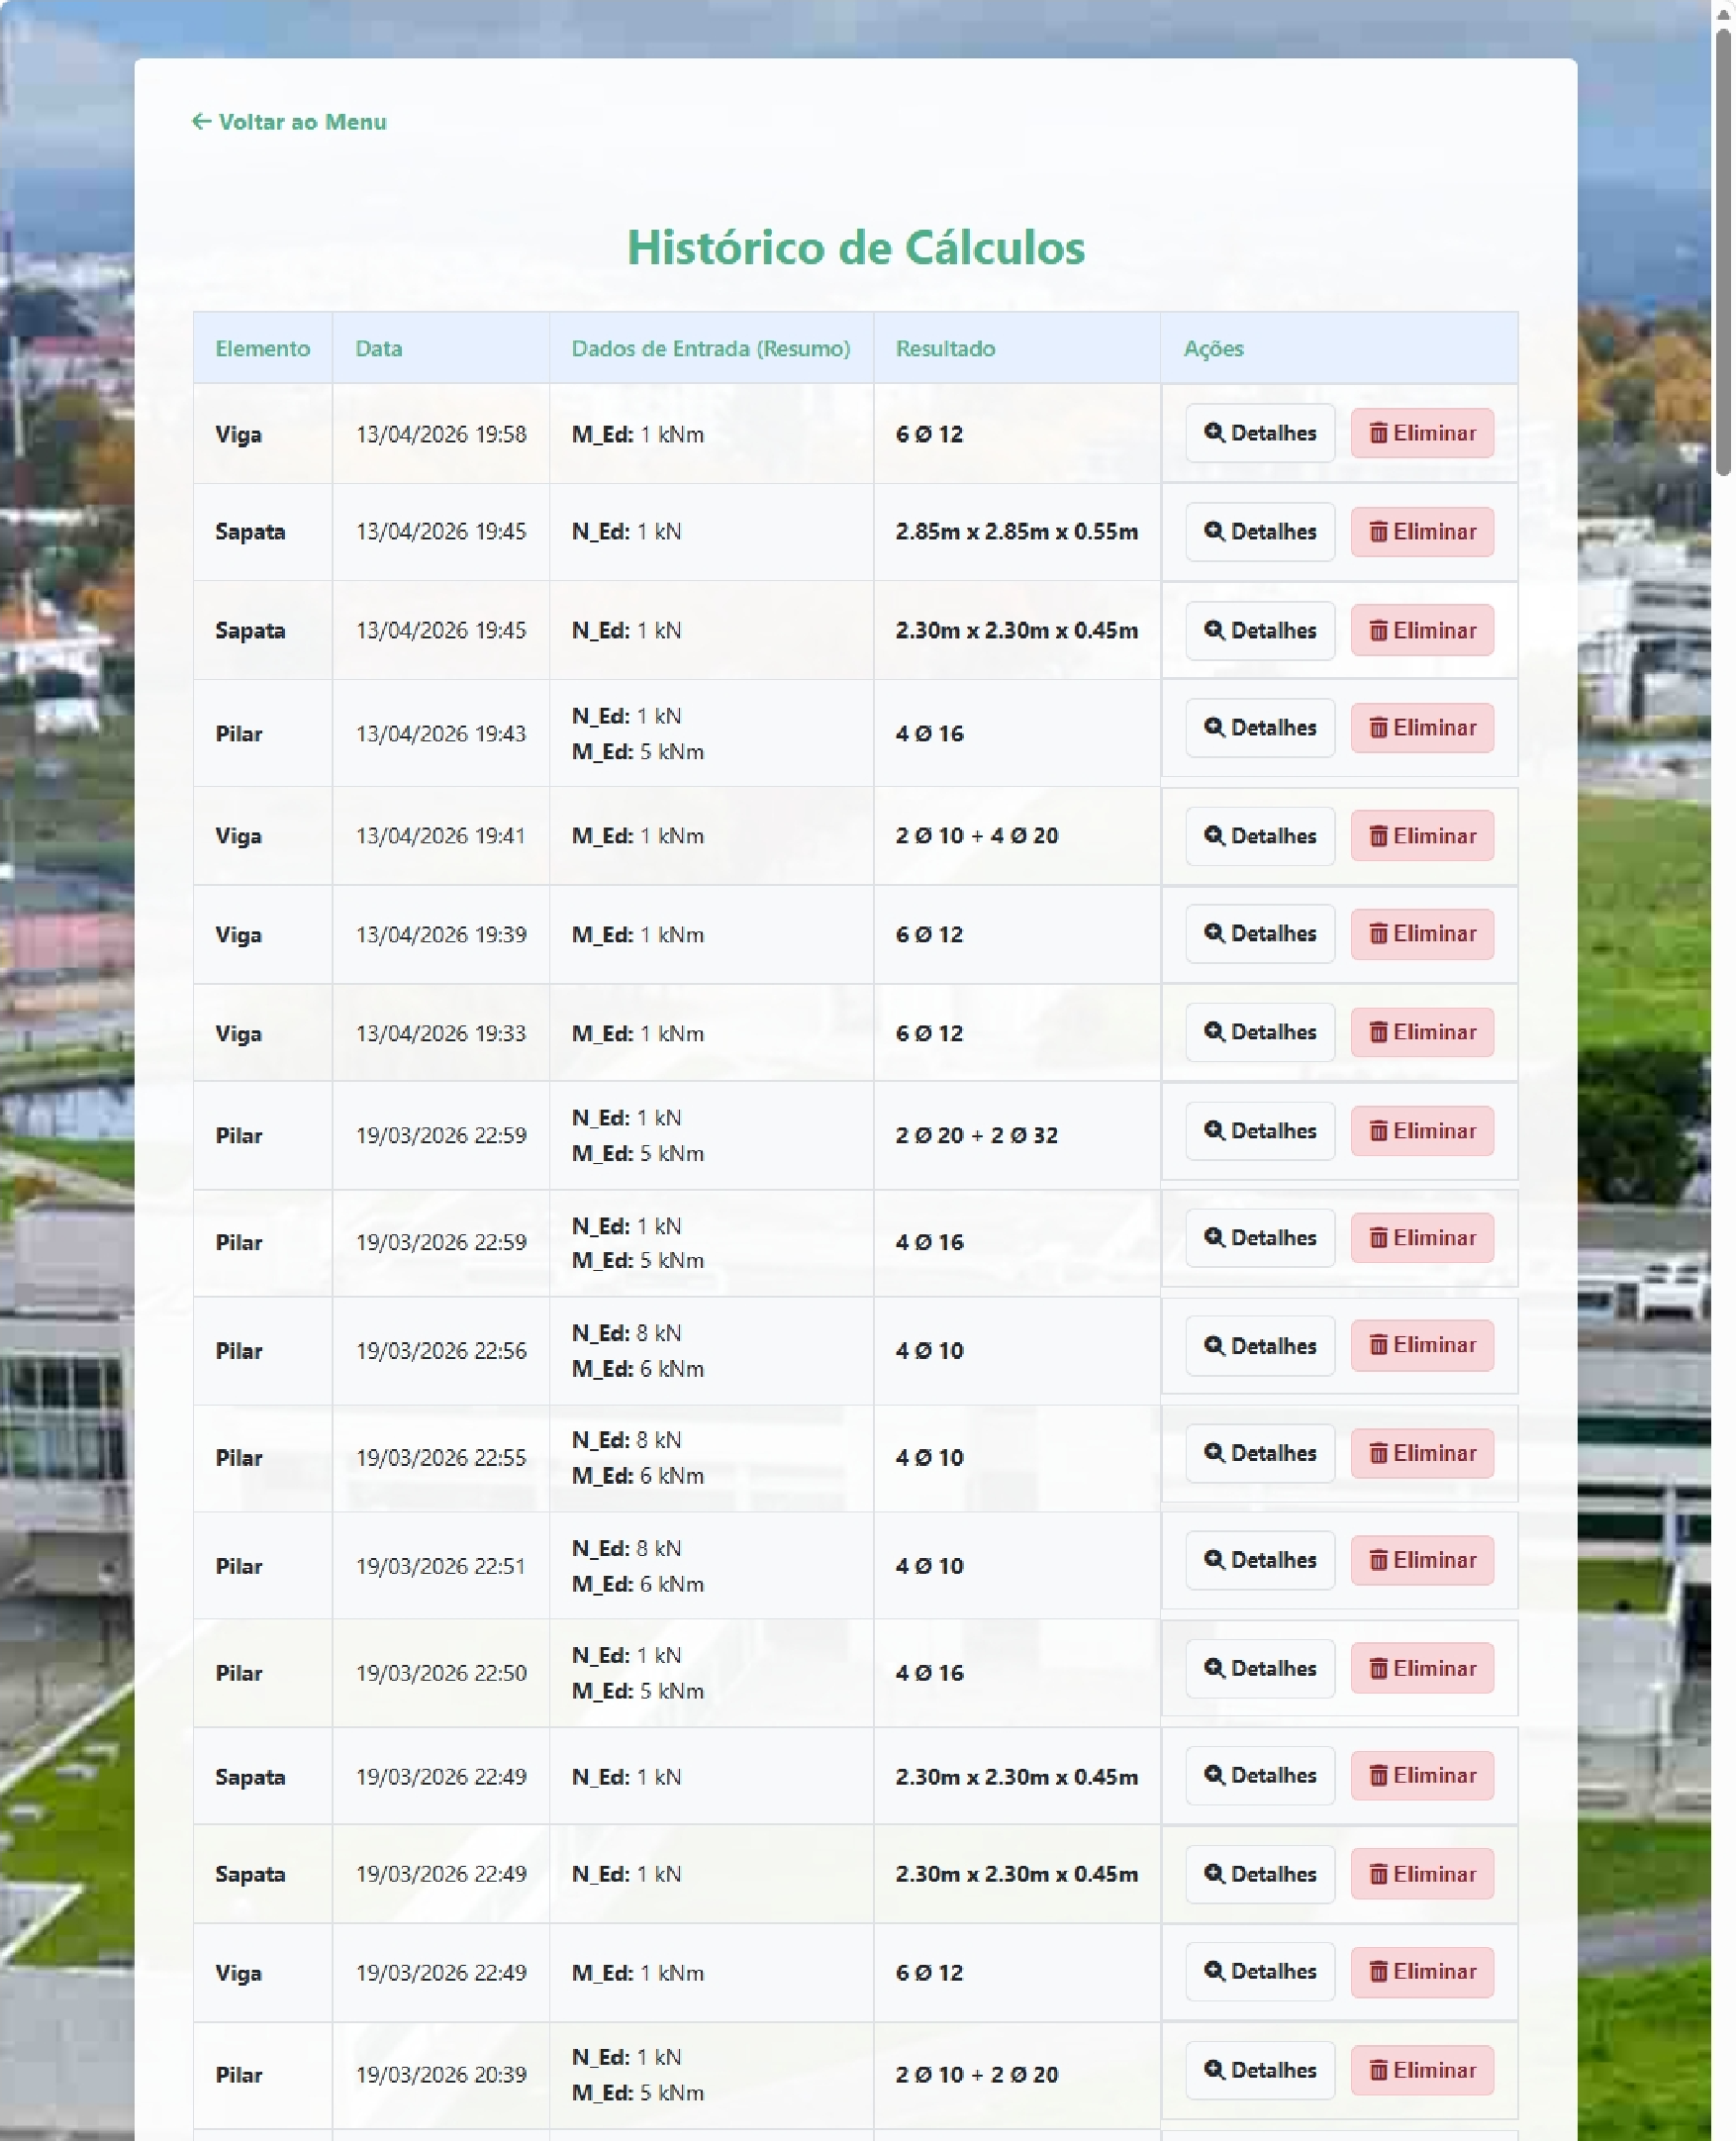
\includepdf[pages=-, pagecommand={}]{Anexos/Interface do histórico de cálculos.pdf}

% =========================================================
% APÊNDICE H
% =========================================================
\newpage
\addcontentsline{toc}{section}{APÊNDICE H - Interface de Configuração do Sistema}
\begin{center}
\section*{APÊNDICE H}
Interface de Configuração do Sistema
\end{center}

O documento seguinte apresenta a interface de configuração do sistema.

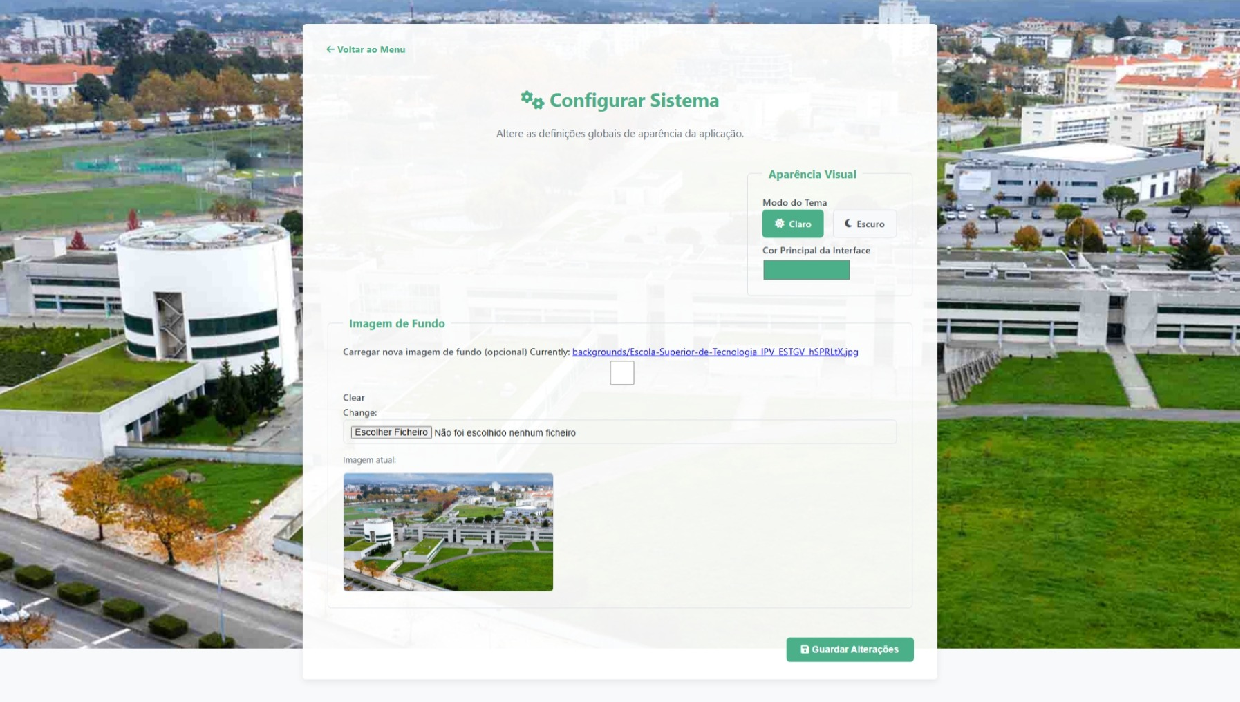
\includepdf[pages=-, pagecommand={}, angle=90]{Anexos/Configurar_Sistema.pdf}

% =========================================================
% APÊNDICE I
% =========================================================
\newpage
\addcontentsline{toc}{section}{APÊNDICE I - Resultado do dimensionamento da viga}
\begin{center}
\section*{APÊNDICE I}
Resultado do dimensionamento da viga
\end{center}

O documento seguinte apresenta o resultado do dimensionamento da viga gerado pela aplicação para o caso de validação correspondente.

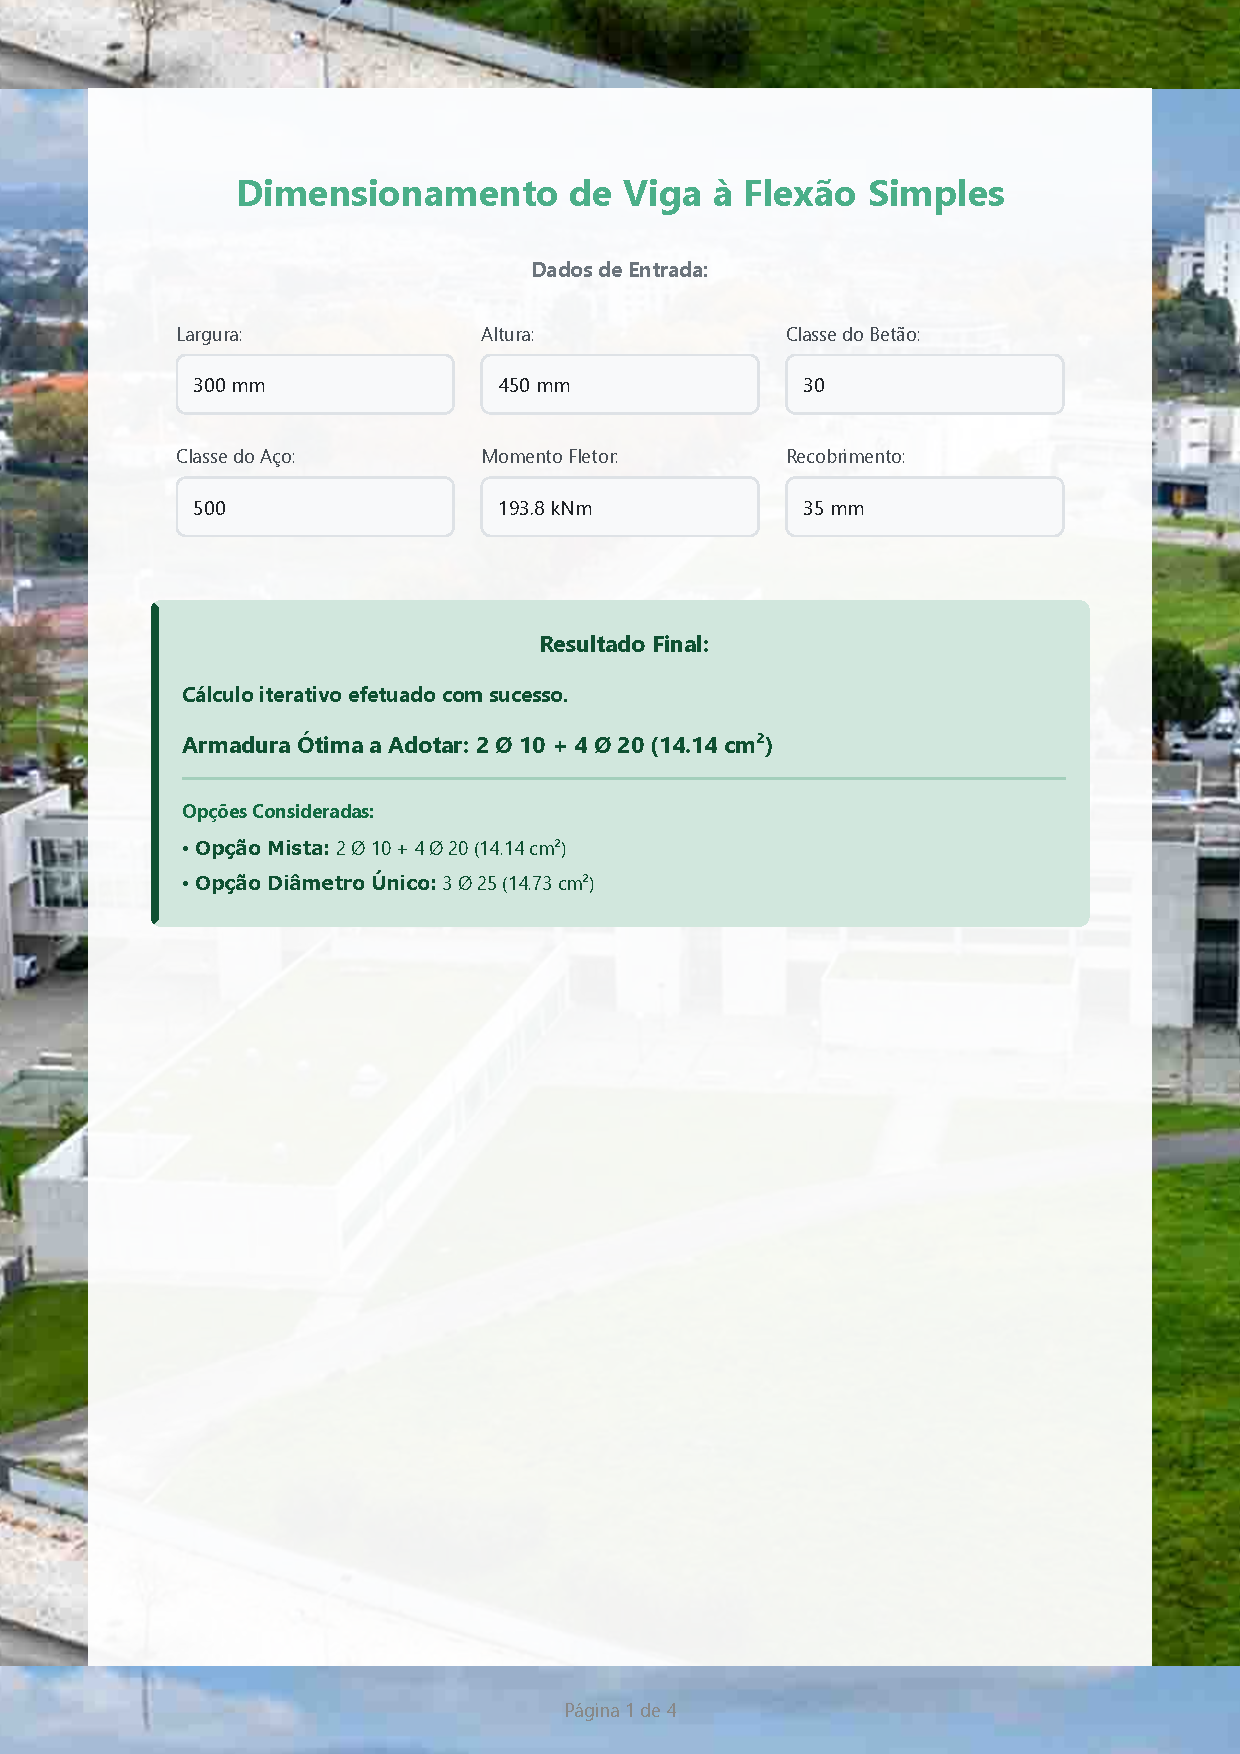
\includepdf[pages=-, pagecommand={}]{Anexos/Relatorio-de-Calculo-Estrutural-_-Viga.pdf}

% =========================================================
% APÊNDICE J
% =========================================================
\newpage
\addcontentsline{toc}{section}{APÊNDICE J - Resultado do dimensionamento do pilar}
\begin{center}
\section*{APÊNDICE J}
Resultado do dimensionamento do pilar
\end{center}

O documento seguinte apresenta o resultado do dimensionamento do pilar gerado pela aplicação para o caso de validação correspondente.

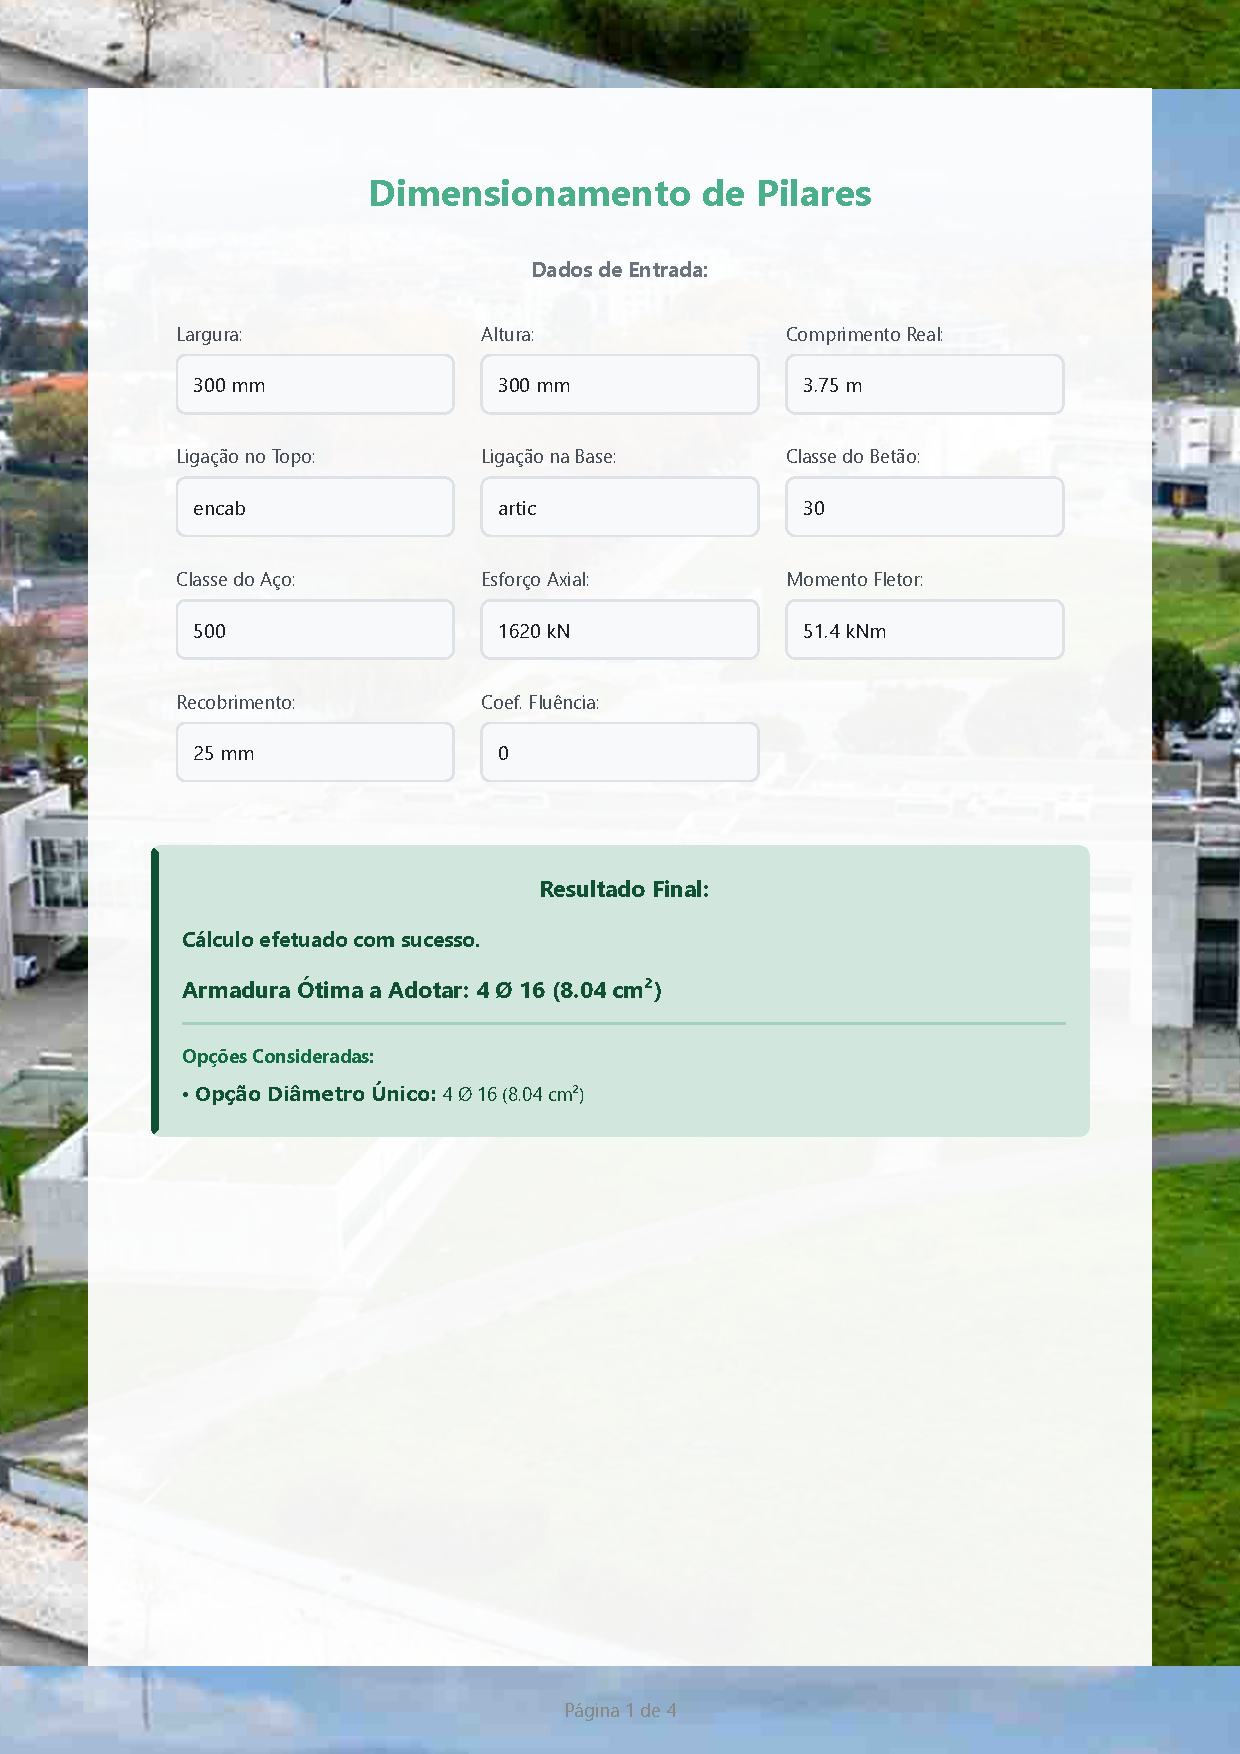
\includepdf[pages=-, pagecommand={}]{Anexos/Relatorio-de-Calculo-Estrutural-_-Pilar-2.pdf}

% =========================================================
% APÊNDICE K
% =========================================================
\newpage
\addcontentsline{toc}{section}{APÊNDICE K - Resultado do dimensionamento da sapata}
\begin{center}
\section*{APÊNDICE K}
Resultado do dimensionamento da sapata
\end{center}

O documento seguinte apresenta o resultado do dimensionamento da sapata gerado pela aplicação para o caso de validação correspondente.

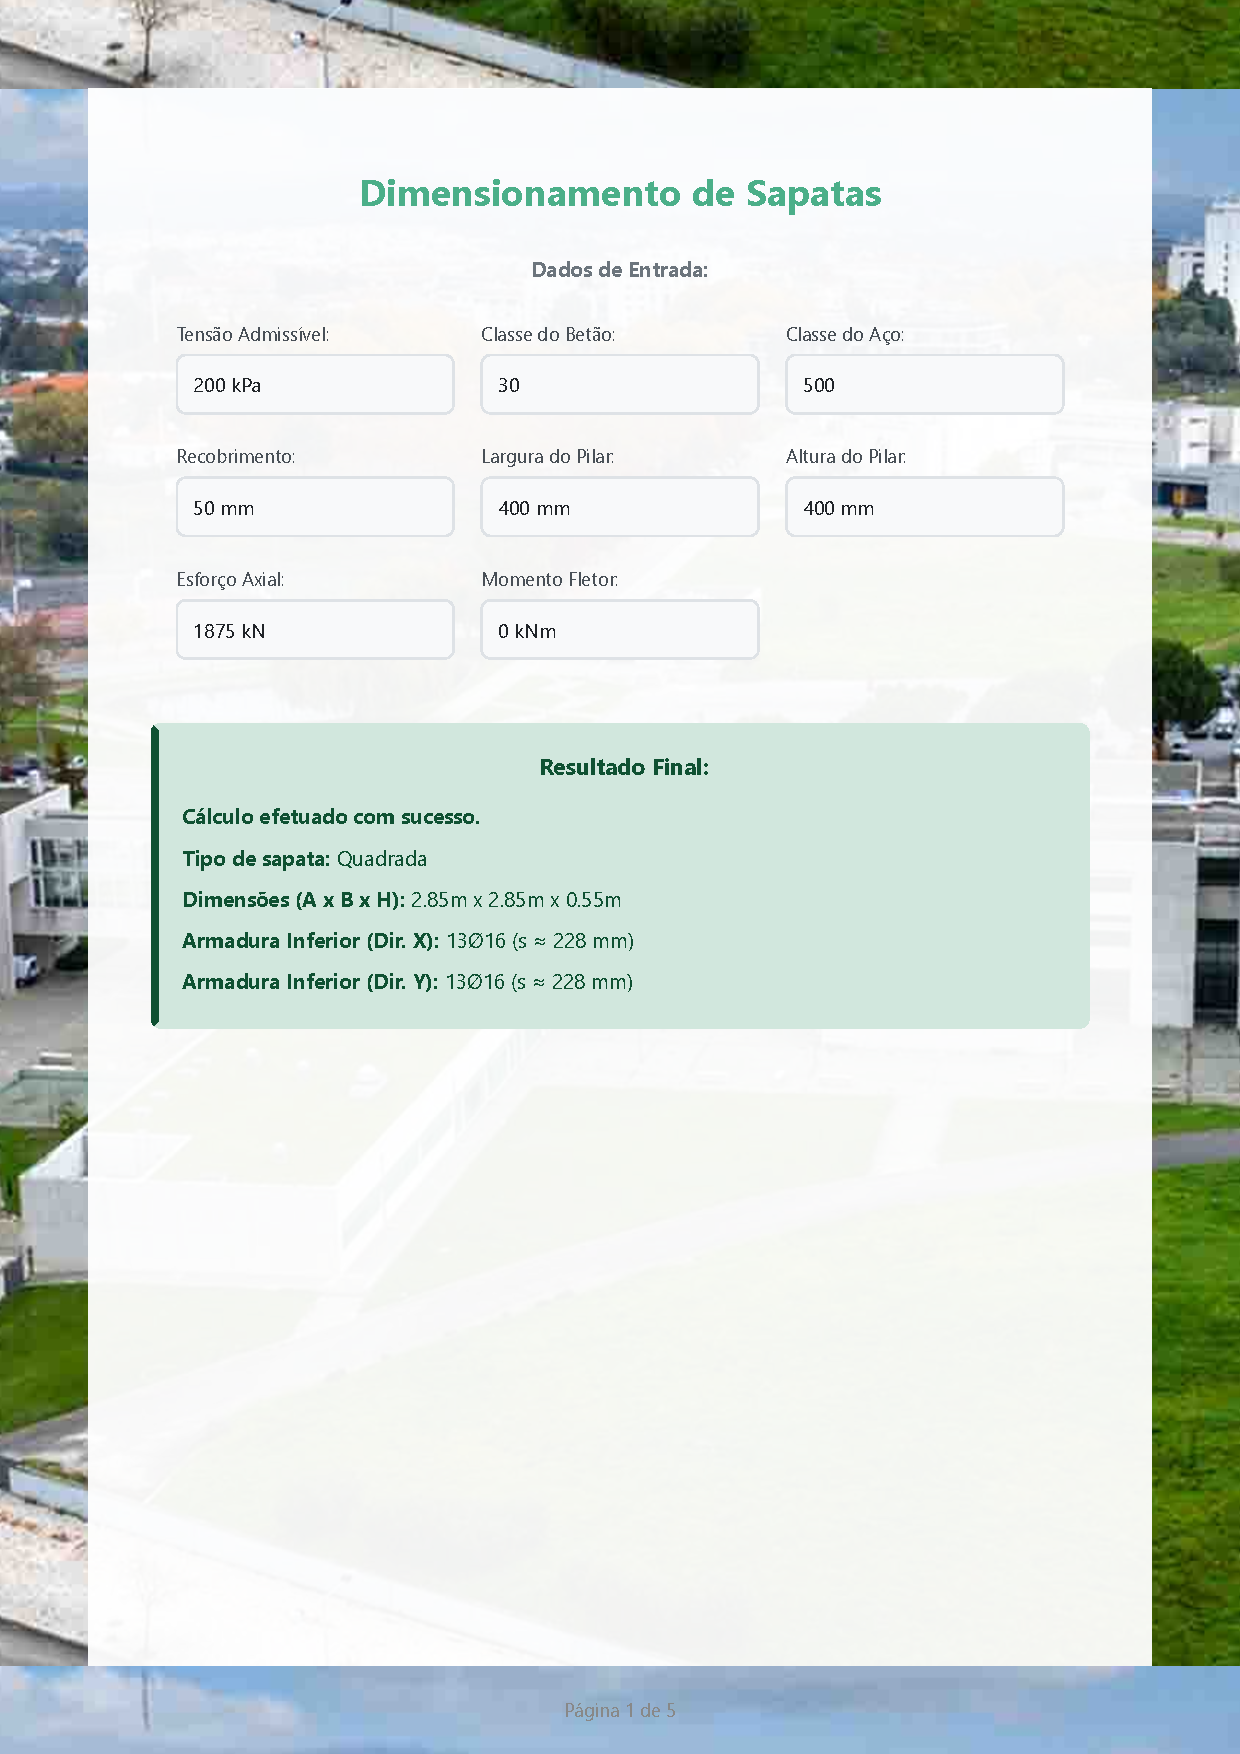
\includepdf[pages=-, pagecommand={}]{Anexos/Relatorio-de-Calculo-Estrutural-_-Sapata-3.pdf}

\end{document}